\documentclass[17pt, a0paper, portrait, margin=10mm, innermargin=15mm, blockverticalspace=15mm, colspace=15mm, subcolspace=8mm]{tikzposter}
%\documentclass[a0paper,17pt]{tikzposter}

\usepackage[utf8]{inputenc}
\usepackage{amsmath}
\usepackage{amsfonts}
\usepackage{amsthm}
\usepackage{amssymb}
\usepackage{mathrsfs}
\usepackage{graphicx}
\usepackage{adjustbox}
\usepackage{enumitem}
\usepackage{multicol}
\usepackage{SUtheme}
\usepackage[sort]{natbib}
\usepackage{wrapfig}
\usepackage{caption}
\usepackage{subcaption}
\usepackage{etoolbox}
\usepackage{ragged2e}

\captionsetup{font=normalsize}

\makeatletter
\newcounter{tablecounter}
\newenvironment{tikztable}[1][]{
	\def \rememberparameter{#1}
	\vspace{10pt}
	\refstepcounter{tablecounter}
	\begin{center}
	}{
		\ifx\rememberparameter\@empty
		\else
		\\[10pt]
		{\small Tab.~\thetablecounter: \rememberparameter}
		\fi
	\end{center}
}
\makeatother

\AtBeginEnvironment{tikzfigure}{\captionsetup{type=figure}}

\setcitestyle{square,numbers}

\usepackage{mwe} % for placeholder images

% set theme parameters
\tikzposterlatexaffectionproofoff
%\usetheme{SUTheme}
\usecolorstyle{SUStyle}
\usetheme{Autumn}
%\usecolorstyle[colorPalette=BrownBlueOrange]{Germany}
\usetitlestyle{Filled}

\usepackage[scaled]{helvet}
\renewcommand\familydefault{\sfdefault} 
\usepackage[T1]{fontenc}


\title{Forward sensitivity analysis of a supercritical extraction process}
\author{Oliwer Sliczniuk, Pekka Oinas, Francesco Corona}
\institute{Aalto University, School of Chemical Engineering}
\titlegraphic{
\includegraphics[width=0.06\textwidth]{aalto_logo.png}}

% begin document
\begin{document}
	\maketitle
	\centering
	\begin{columns}
		\column{0.5}
		
		\block{Introduction}{
				In the supercritical extraction process, a solvent in supercritical conditions is used to separate a solute from solid particles. A distributed-parameter model with three partial differential equations can be used to describe the fluid-solid extraction process. We study the effect of the parameters on the model solution using a forward sensitivity analysis method.
				% The set of additional equations, so called sensitivity equations, is obtained by taking the total derivative of the process model with respect to each parameter. The sensitivity equations are solved simultaneously with the process model. As the results the sensitivity profiles are obtained.
		}
		
%		\block{Supercritical extraction}{
		
%			\begin{minipage}[c]{0.35\linewidth}		
%			The representation of an extractor bed and mass transfer mechanism are shown in figure \ref{SFE_Mechanism}.	\\
%			
%			\begin{itemize} 
%				\item A pre-heated and pressurized solvent (for example $\text{CO}_2$) is pumped through an extractor. 
%				\item The solvent extracts soluble compounds from solid particles as it flows along the fixed bed. 
%				\begin{itemize} 
%					\item The solute diffuses from the particle's core through the solid-fluid interface, the pore, and the film into the bulk.
%				\end{itemize}
%				\item The solvent-solute mixture leaves the operational unit and its pumped to the phase separator.
%			\end{itemize}
%			\end{minipage}
%			\hspace{0.5cm}
%			\vrule
%			\hspace{0.5cm}
%			\begin{minipage}[c]{0.60\linewidth}
%			\begin{tikzfigure}
%				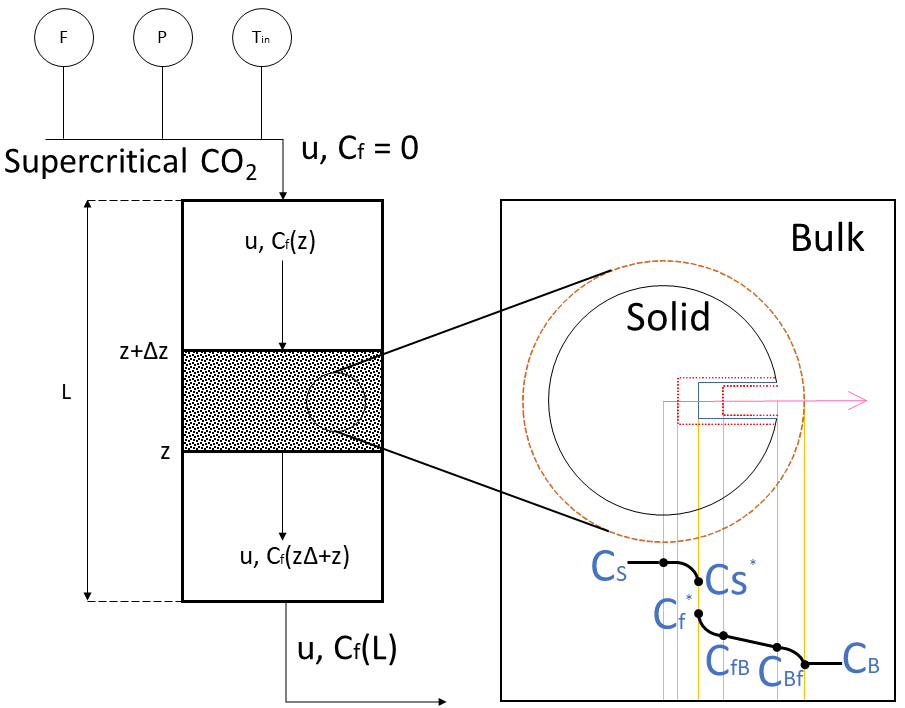
\includegraphics[width=0.75\textwidth]{Figures/SFE_draft_cropped.png}
%				\label{SFE_Mechanism}
%			\end{tikzfigure}
%			\captionof{figure}{Schematic representation of the extracting bed} 
%			\vspace{0.5cm}
%			%The solutes' concentration in the solid phase is denoted as ${\color{blue}c_s}$. The equilibrium concentrations of solid and fluid phases are denoted as ${\color{blue}c_s^*}$ and ${\color{blue}c_f^*}$, respectively. The solute concentration in the fluid in the center of the pore is denoted as ${\color{blue}c_{fB}}$, at the end of the pore as ${\color{blue}c_{Bf}}$ and in the bulk as ${\color{blue}c_B}$.
%			\begin{multicols}{3}
%				\begin{itemize}
%					\item[] ${\color{blue}c_s}$ - solutes' concentration in the core of the particle
%					\item[] ${\color{blue}c_s^*}$ - equilibrium concentrations of solid
%					\item[] ${\color{blue}c_f^*}$ - equilibrium concentrations of fluid
%					\item[] ${\color{blue}c_{fB}}$ - solute concentration in the fluid in the center of the pore
%					\item[] ${\color{blue}c_{Bf}}$ - solute concentration in the fluid at the end of the pore
%					\item[] ${\color{blue}c_B}$ - solute concentration in the bulk 
%				\end{itemize}
%			\end{multicols}
%		\end{minipage}
		

		
			
%		}
		\block{Process model}{
			
			We consider a fluid-solid extraction process model which extends a reference model commonly used in the literature \citep{Reverchon1996}. %The model consists of two mass balance equations related to the concentration of the solute in the fluid and the solid phases, and one heat balance equation related to the pseudo-homogenous phase. 
			\begin{subequations}\begin{align}
					\cfrac{\partial {\color{blue}c_f}(t,z)}{\partial t} &	=  \underbrace{-\cfrac{1}{ {\color{magenta}\varepsilon A}}\cfrac{{\color{red}F}(t)}{{\color{orange}\rho_f}\left[{\color{blue}T}(t,z),{\color{red}P}(t)\right]} \cfrac{\partial {\color{blue}c_f}(t,z)}{\partial {\color{blue}z}}}_{\text{Convective term}} 
					+ \underbrace{ {\color{orange}D^M_e}\left[{\color{blue}T}(t,z),{\color{red}P}(t),{\color{red}F}(t)\right] \cfrac{\partial^2 {\color{blue}c_f}(t,z)}{\partial {\color{blue}z^2}} }_{\text{Diffusive term}} 
					+ \underbrace{ \cfrac{1-{\color{magenta}\varepsilon}}{{\color{magenta}\varepsilon}} {\color{blue}r_e}(t,z) }_{\text{Kinetic term}} \label{eq: Model_fluid} \\
					\cfrac{\partial {\color{blue}c_s}(t,z)}{\partial t} &	= \underbrace{ {\color{blue}r_e}(t,z) }_{\text{Kinetic term}} \label{eq: Model_solid} \\
					\cfrac{\partial {\color{blue}T}(t,z)}{\partial t} &	= \underbrace{ -\cfrac{{\color{red}F}(t) {\color{orange}C_p^f}({\color{blue}T}(t,z),{\color{red}P}(t))}{{\color{magenta}A} [(1-{\color{magenta}\varepsilon}){\color{orange}\rho_f}\left[{\color{blue}T}(t,z),{\color{red}P}(t)\right] {\color{orange}C_p^f} \left[{\color{blue}T}(t,z),{\color{red}P}(t)\right] + {\color{magenta}\varepsilon}{\color{magenta}\rho_s}{\color{magenta}C_p^s } ]} \cfrac{\partial {\color{blue}T}(t,z)}{\partial {\color{blue}z}}  }_{\text{Convective term}} 
					+ \underbrace{ {\color{orange}D^T_e}\left[{\color{blue}T}(t,z),{\color{red}P}(t)\right] \cfrac{\partial^2 {\color{blue}T}(t,z)}{\partial {\color{blue}z^2}} }_{\text{Diffusive term}} \label{eq: Heat_balance}
			\end{align}\end{subequations}
		
	\vspace{1.4cm}
			
%			where ${\color{blue}c}(t,z)$, ${\color{blue}q}(t,z)$, and ${\color{blue}T}(t,z)$ denote the concentration of solute in the fluid, concentration of solute in the solid, and temperature of the pseudo-homogenous phase at time $t$ and axial position $z$ along the bed, respectively. ${\color{red}F}(t)$ denotes the mass flow-rate along the extractor and ${\color{red}P}(t)$ is the pressure. ${\color{magenta}\epsilon}$ denotes the void fraction of the bed, ${\color{magenta}\rho_s}$ is the density of the solid phase, and ${\color{magenta}A}$ is the extractor’s cross section. ${\color{orange}\rho_f}\left[{\color{blue}T}(t,z),{\color{red}P}(t)\right]$ denotes the density of the fluid phase, ${\color{orange}D^M_e}\left[{\color{blue}T}(t,z),{\color{red}P}(t),{\color{red}F}(t)\right]$ is the axial mass diffusion coefficient, ${\color{orange}C_p^f}\left[{\color{blue}T}(t,z),{\color{red}P}(t)\right]$ is the specific heat of the fluid phase, and ${\color{orange}D_e^T}\left[{\color{blue}T}(t,z),{\color{red}P}(t)\right]$ is the axial heat diffusion coefficient. ${\color{magenta}C_p^s}$ denotes the specific heat of the solid particles. 
			
%			\begin{tikztable}
%				\centering
%				\begin{tabular}{p{0.325\linewidth}|p{0.325\linewidth}|p{0.325\linewidth}}
%					\hline
%					${\color{blue}c}(t,z)$	&  ${\color{blue}q}(t,z)$ & ${\color{blue}T}(t,z)$  \\
%					 Solute's concentration in the fluid phase & Solute's concentration in the solid phase & Temperature of the pseudo-homogeneous phase \\
%					 \hline
%				\end{tabular}
%				\begin{tabular}{p{0.19\linewidth}|p{0.19\linewidth}|p{0.19\linewidth}|p{0.19\linewidth}|p{0.19\linewidth}}
%					${\color{red}F}(t)$ & ${\color{red}P}(t)$	& ${\color{magenta}\epsilon}$ & ${\color{magenta}\rho_s}$ & ${\color{magenta}A}$ \\
%					Solvent flow rate & Pressure & Void fraction & Density of the solid particles & Extractor's cross-section \\ 
%					\hline
%				\end{tabular}	
%				\begin{tabular}{p{0.19\linewidth}|p{0.19\linewidth}|p{0.19\linewidth}|p{0.19\linewidth}|p{0.19\linewidth}}
%					 ${\color{orange}\rho_f}\left[{\color{blue}T}(t,z),{\color{red}P}(t)\right]$& 					${\color{orange}D^M_e}\left[{\color{blue}T}(t,z),{\color{red}P}(t),{\color{red}F}(t)\right]$ & ${\color{orange}C_p^f}\left[{\color{blue}T}(t,z),{\color{red}P}(t)\right]$ & ${\color{orange}D_e^T}\left[{\color{blue}T}(t,z),{\color{red}P}(t)\right]$ & ${\color{magenta}C_p^s}$ \\
%					Density of the solvent & Axial mass diffusion factor & Specific heat of the fluid phase & Axial heat diffusion factor & Specific heat of the solid particles \\
%					\hline
%				\end{tabular}
%			\end{tikztable}
%			\captionof{table}{Symbols used in the process model}
	

			\begin{multicols}{2}
				\begin{itemize}
					\item[] ${\color{blue}c_f}(t,z)$ - Concentration of the solute in the solvent [$kg~m^{-3}$]
					\item[] ${\color{blue}c_s}(t,z)$ - Concentration of the solute in the solid phase [$kg~m^{-3}$]
					\item[] ${\color{blue}T}(t,z)$ - Temperature of the pseudo-homogeneous phase [$^\circ C$]
					\item[] ${\color{red}F}(t)$ - Flow rate of the solvent [$kg~s^{-1}$]
					\item[] ${\color{red}P}(t)$ - Pressure [$bar$]
					\item[] ${\color{magenta}A}$ - Cross-section of the extractor [$m^2$]
					\item[] ${\color{magenta}\epsilon}$ - Void fraction [$-$]
					\item[] ${\color{magenta}\rho_s}$ - Density of the solid particles [$kg~m^{-3}$]
					\item[] ${\color{orange}\rho_f}\left[{\color{blue}T}(t,z),{\color{red}P}(t)\right]$ - Density of the solvent [$kg~m^{-3}$]
					\item[] ${\color{orange}D^M_e}\left[{\color{blue}T}(t,z),{\color{red}P}(t),{\color{red}F}(t)\right]$ - Axial mass diffusion coefficient of the solute in the solvent [$m^2 ~ s^{-1}$]
					\item[] ${\color{orange}C_p^f}\left[{\color{blue}T}(t,z),{\color{red}P}(t)\right]$ - Specific heat of the solvent [$J~mol^{-1}~K^{-1}$]
					\item[] ${\color{orange}D_e^T}\left[{\color{blue}T}(t,z),{\color{red}P}(t)\right]$ - Axial heat diffusion coefficient of the pseudo-homogenous phase [$m^2 ~ s^{-1}$]
					\item[] ${\color{magenta}C_p^s}$ - Specific heat of the solid phase [$J ~ mol^{-1} ~ K^{-1}$]
				\end{itemize}
			\end{multicols}
		
		\vspace{1.0cm}
		\hrule
		\vspace{1.5cm}
		
		%		The movement of the solvent and the pseudo-homogeneous phase is considered only in the axial direction. The perfect mixing in the radial direction is assumed. In addition, if the boundary layer adjacent to the inner wall of the extractor does not exist, then the velocity profile is constant across any cross-section of the extractor perpendicular to the axial direction. As a result, the plug flow model can be introduced. The particle size distribution and the void fraction of the solid phase are assumed to be uniform in space and remain constant in time. Moreover, the pressure is assumed to be constant along the extractor. 
		
			\textit{Model assumptions and description}
			
			\begin{multicols}{2}
				\begin{itemize}
					\item One-dimensional model
					%					\item Movement in the axial direction
					\item No radial profiles
					\item Plug flow 
					\item No pressure drop
					%					\item Negligible external diffusion 
					\item Uniform particle size distribution
					\item Constant particle-size and void fraction
					\item Single component solute
					\item The amount of solute in the solvent is considered negligible
					\item Two-film theory
					\item Pseudo-homogeneous thermal properties
				\end{itemize}
			\end{multicols}
		
%		 The mass balance equation of the fluid phase (Eq. \ref{eq: Model_fluid}) consists of convective, diffusive and kinetic terms. The mass balance equation of the solid (Eq. \ref{eq: Model solid}) phase has only the kinetic term because the solid particles are fixed. 

				\vspace{1.5cm}

				The solvent flows through a fixed bed of solid particles and dissolves the soluble substances. We consider the axial dispersion of the solute in the solvent and assume that radial dispersion is negligible. The mass balance for the fluid phase (Eq. \ref{eq: Model_fluid}) consist of convection, diffusion, and kinetic terms.\\
				
				The solid phase is fixed, which indicates lack of a convective movement of the solid particles. We assume that the diffusion of the solute between solid particles is negligible. The mass balance for the solid phase (Eq. \ref{eq: Model_solid}) consist of the kinetic term only.% Therefore, the only term present in this equation is the kinetic term (defined as presented in Eq. \ref{Model_kinetic_basic}), which links solid and fluid phases.
				
				\begin{itemize}
					\item The mass transfer kinetic (Eq. \ref{Model_kinetic_basic}) describe a diffusion rate of the solute from solid particles to the solvent. The kinetic term consists of the overall diffusion coefficient and the concentration gradient, which acts as a driving force for the process.
					
%					\begin{minipage}[c]{0.5\linewidth}
%					
%					\end{minipage}
%%
%				\begin{multicols}{2}
%					\begin{itemize}
%						\item[] ${\color{orange}D_i}({\color{blue}T}(t,z))$ - overall diffusion coefficient [$m^2 ~ s^{-1}$]
%						\item[] ${\color{magenta}\mu}$ - shape coefficient [$-$]
%						\item[] ${\color{magenta}l}$ - characteristic dimension of particles [$m$]
%						\item[] ${\color{orange}k_m}({\color{blue}T}(t,z))$ - mass partition factor [$-$]
%					\end{itemize}
%				\end{multicols} 

			\end{itemize}		
				\begin{minipage}[c]{0.5\linewidth}
					\begin{equation}
						{\color{blue}r_e}(t,z) = -\cfrac{{\color{orange}D_i}({\color{blue}T}(t,z))}{{\color{magenta} \mu l^2} }\left({\color{blue}c_s}(t,z) - \cfrac{{\color{magenta}\rho_s}}{{\color{orange}k_m}\left[{\color{blue}T}(t,z)\right]{\color{orange}\rho_f}\left[{\color{blue}T}(t,z),{\color{red}P}(t)\right]}  {\color{blue}c_f}(t,z) \right) \label{Model_kinetic_basic}
					\end{equation}
				\end{minipage}
				\hspace{2.0cm}
				\begin{minipage}[c]{0.44\linewidth}	
					\vspace{0.2cm}
					\begin{itemize}
						\item[] ${\color{orange}D_i}({\color{blue}T}(t,z))$ - Overall diffusion coefficient [$m^2 ~ s^{-1}$]
						\item[] ${\color{magenta}\mu}$ - Shape coefficient [$-$]
						\item[] ${\color{magenta}l}$ - Characteristic dimension of particles [$m$]
						\item[] ${\color{orange}k_m}({\color{blue}T}(t,z))$ - Mass partition factor [$-$]
					\end{itemize}
				\end{minipage}
			\vspace{1.0cm}
			\hrule
			\vspace{1.0cm}
				\begin{minipage}[c]{0.5\linewidth}
					\begin{tikzfigure} \label{SFE_MassTransfer}
						\centering
						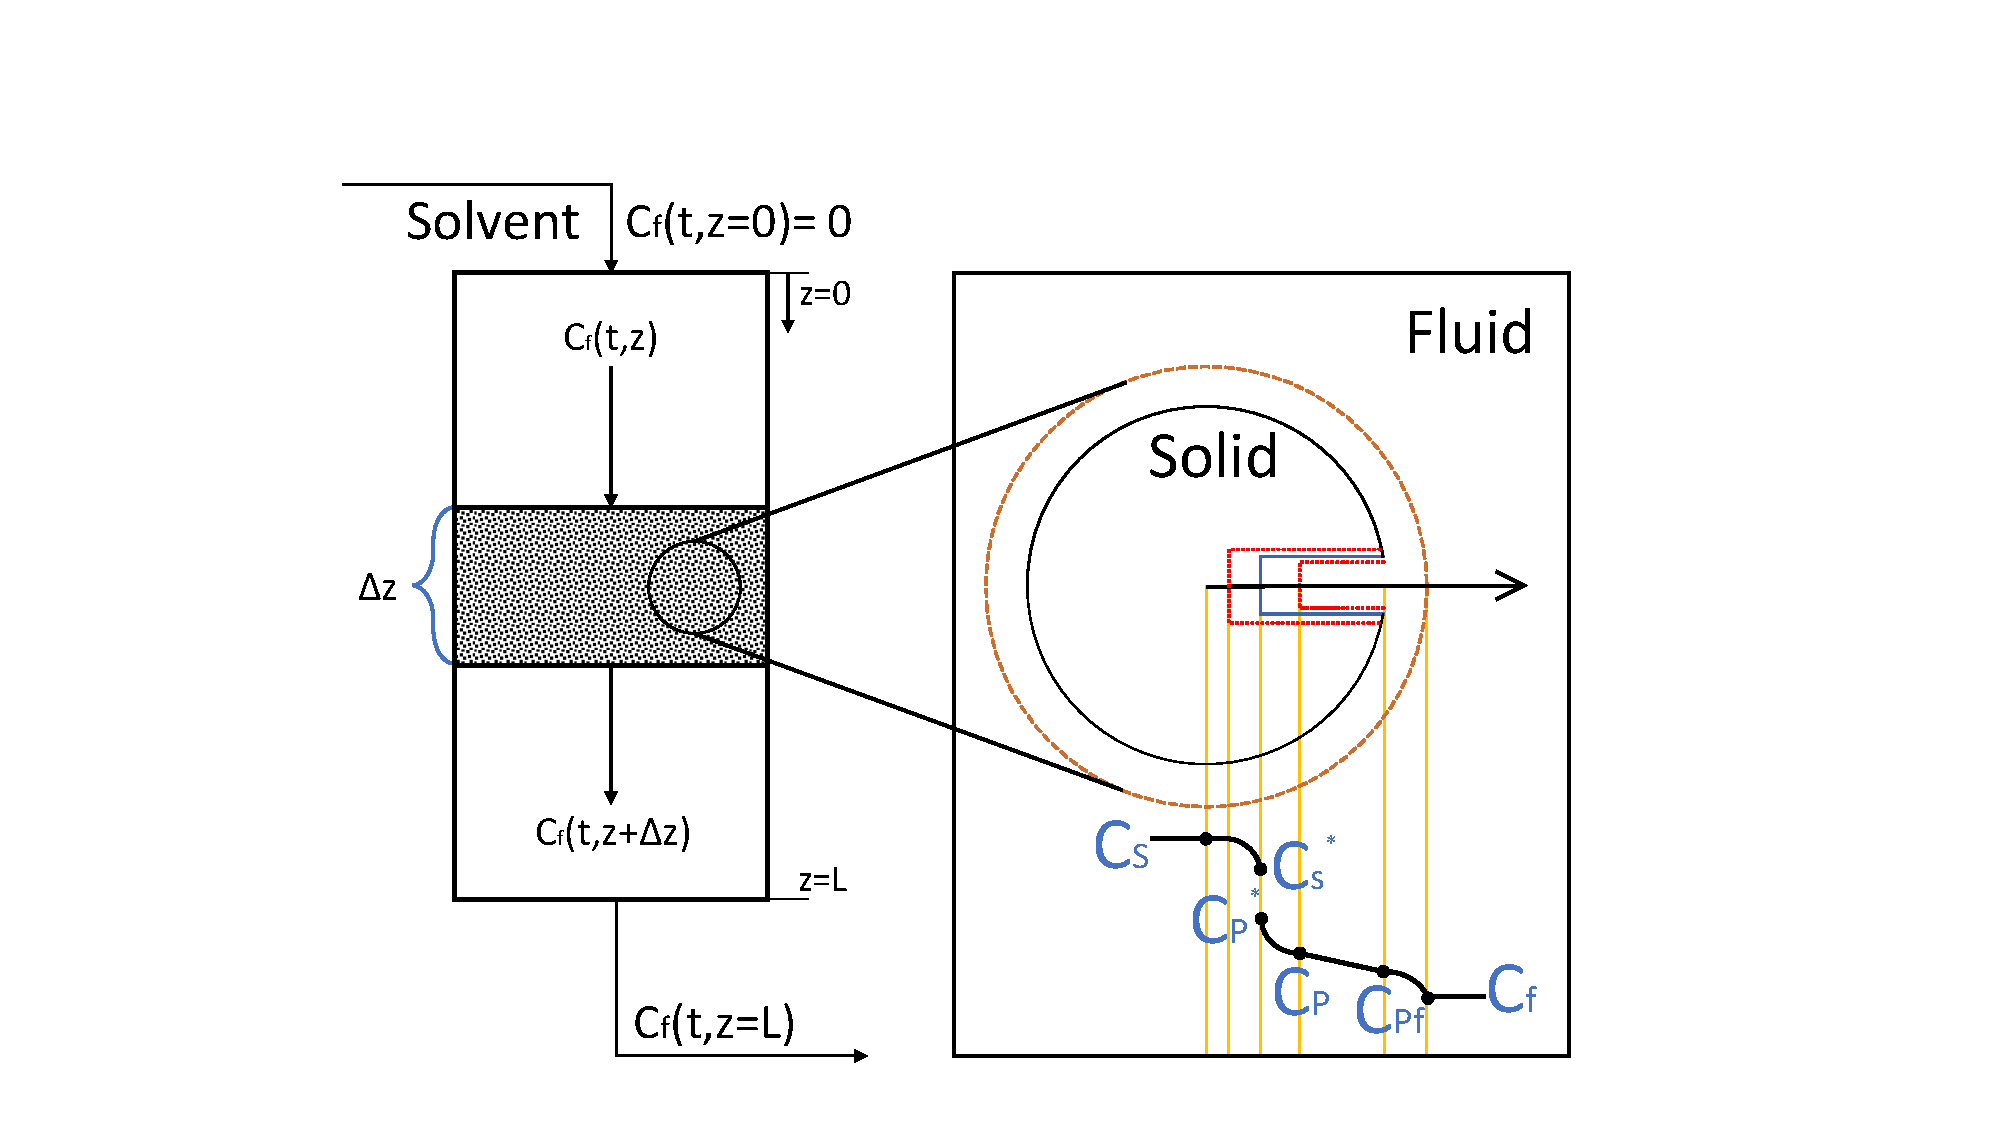
\includegraphics[trim = 5.8cm 1.1cm 6cm 0.8cm,clip,width=1.0\linewidth]{Figures/SFE_draft.pdf}
						\label{SFE_Mechanism}
					\end{tikzfigure}
					\captionof{figure}{Schematic representation of the extracting bed} 
				\end{minipage}
				\hspace{2.0cm}
				\begin{minipage}[c]{0.44\linewidth}
					\vspace{0.2cm}
						\begin{itemize}
							\item[] $L$ - Length of the fixed bed
							\item[] $z$ - Axial coordinate of the fixed bed
							\item[] $\Delta z$ - Length interval
						\end{itemize}
%					\vspace{-0.25cm}
					\hrule
					\begin{itemize}
						\item[] ${\color{blue}c_s}$ - Concentration of the solute in the core of the particle
						\item[] ${\color{blue}c_s^*}$ - Equilibrium concentrations of the solute in the solid phase at the solid-fluid interface
						\item[] ${\color{blue}c_P^*}$ - Equilibrium concentrations of the solute in the fluid phase at the solid-fluid interface
						\item[] ${\color{blue}c_{P}}$ - Concentration of the solute in the fluid phase in the centre of the pore
						\item[] ${\color{blue}c_{Pf}}$ - Concentration of the solute in the fluid phase at the end of the pore
						\item[] ${\color{blue}c_f}$ - Concentration of the solute in the solvent 
						\vspace{0.2cm}
						\hrule
					\end{itemize}
				\end{minipage}
					
%					${\color{orange}D_i}({\color{blue}T}(t,z))$ corresponds to the overall diffusion coefficient. ${\color{magenta}\mu}$ denotes the shape coefficient, ${\color{magenta}l}$ is the characteristic dimension of particles and ${\color{orange}k_m}({\color{blue}T}(t,z))$ is the mass partition factor.
					
			\vspace{1.5cm}
			
			The heat balance (Eq. \ref{eq: Heat_balance}) consists of the convective and diffusive terms. It follows the assumption of a pseudo-homogeneous phase, which properties are the mean between fluid and solid phases. We consider that there is no heat loss through the wall, and there is no heat generation in the system. The temperature of the extractor can be changed only by manipulating the temperature of the inlet stream ${\color{red}T_{Inlet}}(t)$.
			
			\vspace{1.0cm}
			\hrule
			\vspace{1.5cm}
			
			
			\textit{Observations}: 
			
%			The process performance is indicated by the measurement equation (Eq. \ref{eq: Yield}). The yield is based on the solute concentration in the solid phase. It is calculated as the ratio between the difference of its initial value ${\color{magenta}c_s^0}$ and the actual value, compared to the initial one.
			
			The efficiency of the process (the yield) is calculated according to Eq. \ref{eq: Yield}, and is based on the change of solutes concentration in the solid phase. It is defined as ratio the ratio between the difference of its initial value ${\color{magenta}c_s^0}$ and the actual value ${\color{blue}c_s}(t,z)$, compared to the initial one.
			
			\begin{equation}
				{\color{blue}y}(t) = \cfrac{\left({\color{magenta}c_s^0} - {\color{blue}c_s}(t,z) \right) }{{\color{magenta}c_s^0}} 100\% \label{eq: Yield}
			\end{equation}
			
%			The volume of the extractor is ${\color{magenta}V}$. The ${\color{magenta}q_0}$ is the initial concentration of the solute in the solid phase. \\

%			\begin{center} ${\color{magenta}V}$ - volume of the extractor [$m^3$] ~ ${\color{magenta}q_0}$ - initial concentration of the solute in the solid phase [$kg m^{-3}$] \end{center}
			
			%        \textcolor{blue}{State variables}, \textcolor{red}{control variables}, \textcolor{magenta}{parameters}, \textcolor{orange}{other variables}
			
			\vspace{1.0cm}
			\hrule
			\vspace{1.5cm}
			
			\textit{Numerics}: 
			
			The method of lines is used to transform the process model equations into a set of ODEs denoted as ${\color{blue}G}({\color{blue}x}(t);{\color{magenta}\theta})$, where ${\color{blue}x}(t)$ is the discretized state and the ${\color{magenta}\theta}$ represents the collection of model parameters and the control variables (assuming they are constant). 
			
			The partial derivatives in $z$-direction are computed using a first-order and second-order finite difference approximation. The backward finite difference is used to approximate first-order derivatives, while the central difference scheme is used to approximate second-order derivatives.
			
			The length of the fixed bed is divided into $N_z$ equally distributed points in the $z$-direction. 
			
		}
		
		\column{0.5}
		
		\block{Sensitivity analysis}{
			
			The sensitivity analysis aims to measure the effect of the parameters on process model solution. The sensitivity analysis equations (${\color{blue}\dot{Z}}$) are obtained by taking the total derivative of the discretized system ${\color{blue}G}({\color{blue}x}(t);{\color{magenta}\theta})$ with respect to ${\color{magenta}\theta}$, as presented in \citep{Maly1996}. In this work, the direct method is considered and restricted to the analysis of linear sensitivity coefficients.
			
			\begin{align} \label{SA_def}
				{\color{orange}Z}({\color{blue}x}(t);{\color{magenta}\theta}) &= \cfrac{\partial {\color{blue}x}(t)}{\partial {\color{magenta}\theta}}
			\end{align}
			
			As the process model depends on parameters ${\color{magenta}\theta}$ and initial conditions, each parameter's sensitivity depends on time $t$. Therefore, the new system of equations can be obtained by taking derivatives with respect to time $t$ and applying the chain rule.
			
			\begin{equation} \label{SA_dt} 
				{\color{blue}\dot{Z}}({\color{blue}x}(t);{\color{magenta}\theta})  = \cfrac{d {\color{orange}Z}(x(t);{\color{magenta}\theta})}{d t} = \cfrac{\partial }{\partial t} \left( \cfrac{\partial {\color{blue}x}(t)}{\partial {\color{magenta}\theta}} \right) = \cfrac{\partial }{\partial {\color{magenta}\theta}} \left( \cfrac{\partial {\color{blue}x}(t)}{\partial t} \right) = \cfrac{d {\color{blue}G}({\color{blue}x}(t);{\color{magenta}\theta})}{d {\color{magenta}\theta}} 
			\end{equation}
			
			By applying the definition of the total derivative to the Eq. \ref{SA_dt}, the sensitivity equation can be obtained.
			
			\begin{align}		
				\label{SA_eq_full}\cfrac{d {\color{blue}G}({\color{blue}x}(t);{\color{magenta}\theta})}{d {\color{magenta}\theta}} &=  \underbrace{ \cfrac{\partial {\color{blue}G}({\color{blue}x}(t);{\color{magenta}\theta})}{\partial {\color{blue}x}(t)} }_{{\color{blue}J_x}({\color{blue}x}(t);{\color{magenta}\theta})} \underbrace{\cfrac{\partial {\color{blue}x}(t)}{\partial {\color{magenta}\theta}} }_{{\color{blue}S}({\color{blue}x}(t);{\color{magenta}\theta})} + \underbrace{ \cfrac{\partial {\color{blue}G}({\color{blue}x}(t);{\color{magenta}\theta})}{\partial {\color{magenta}\theta}} }_{{\color{blue}J_p}({\color{blue}x}(t);{\color{magenta}\theta})}
			\end{align}
			
			This equation consists of three terms: Jacobian ${\color{blue}J_x}({\color{blue}x}(t);{\color{magenta}\theta})$, sensitivity matrix ${\color{blue}S}({\color{blue}x}(t);{\color{magenta}\theta})$ and Jacobian ${\color{blue}J_p}({\color{blue}x}(t);{\color{magenta}\theta})$. The Jacobians are obtained by automatic differentiation. The sensitivity equations are coupled with the process model and solved simultaneously. As the result,  the gradients of the solution with respect to each parameter along the time series are obtained.
			
%			Given the system of $N_x$ ordinary differential equations $\dot{x}(t) = f\left(x(t)|u_\text{const},\theta\right)$ resulting from the space discretisation of the process model, Eq. {\color{red}REF}, where $f : \mathbb{R}^{N_x} \to \mathbb{R}^{N_x}$ is the vector field, $u_\text{const} \in \mathbb{R}^{N_u}$ and $\theta \in \mathbb{R}^{N_\theta}$ are constant controls and model parameters collectively denoted as $p \in \mathbb{R}^{N_p = N_u + N_\theta}$, we simultaneously solve for both $\{x_{n_x}(t)\}_{n_x=1}^{N_x}$ and a set of sensitivity functions $\left\{ \partial{x_{n_x}(t)} / \partial{p_{n_p}}\right\}_{n_p=1}^{N_p}$ for $t \ge 0$. The partial derivatives measure the sensitivity of the solution with respect to individual changes in the parameters $\{p_{n_p}\}_{n_p=1}^{N_p}$, over time. These functions are obtained by solving an additional set of ordinary differential equations called sensitivity equations. To determine the effect of the parameters, we consider the direct method ({\color{red}{REFS}}) and restrict our analysis to a first-order sensitivity analysis. Though, directed method can be used to execute higher-order analysis, their usefulness is seldom emphasised {\color{red}{REF}}; Therefore, we only compute linear sensitivity coefficients.
%			
%			The original system of $N_x$ ODEs has solutions $\{x_{n_x}(t \ge 0)\}$  that are dependent on the parameters $p$ as well as on the initial conditions $\{x_{n_x}(t=0)\}$. As such solutions are understood as functions of both time $t$ and the parameters $p$ (that is, $x_{n_x}\left(t \ge 0|p\right)$), to determine their sensitivity to each parameter $p_{n_p}$, we introduce $N_x$ new variables $\{z_{n_x}(t| p_{n_p})\}_{n_x=1}^{N_x}$ with $z_{n_x}(t|p_{n_p}) \in \mathbb{R}^{N_p}$ and such that $z_{n_x}(t|p_{n_p}) = \partial{x_{n_x}(t)} / \partial{p_{n_p}}$, for $n_p=1,\dots,N_p$. The functions $z_{n_x}(t \ge 0|n_p)$ are obtained as solutions to $N_x$ sensitivity differential models $\{\dot{z}_{n_p}(t | p_{n_p}) = h_{n_p}\left(z_{n_p}(t|p_{n_p}),x(t)|p\right)\}$ to be solved simultaneously with $\dot{x}(t) = f\left(x(t)|p\right)$, from an appropriate set of conditions $\{z_{n_x}(t=0 | p_{n_p})\}$. Each sensitivity model $\dot{z}_{n_x}(t|p_{n_p}) = h_{n_p}\left(z_{n_x}(t|p_{n_p}),x(t)|p\right)$ is given by
%			\begin{align}\begin{split}
%					\dot{z}_{n_x}(t|p_{n_p}) & = \cfrac{\partial{z_{n_x}(t | p_{n_p})}}{\partial{t}} \\
%					& = \cfrac{\partial}{\partial{t}}\left(\cfrac{\partial{x_{n_x}(t)}}{\partial{p_{n_p}}}\right) \\
%					& = \cfrac{\partial}{\partial{p_{n_p}}}\left(\cfrac{\partial{x_{n_x}(t)}}{\partial{t}}\right) \\
%					& = \cfrac{\partial}{\partial{p_{n_p}}}\left(f_{n_x}\left(x(t)|p\right)\right) \\
%					& = \cfrac{\partial{f_{n_x}\left(x(t)|p\right)}}{\partial{p_{n_p}}} + \sum_{\overline{n_x} = 1}^{N_x}{\cfrac{\partial{f_{n_x}\left(x(t)|p\right)}}{\partial{x_{\overline{n_x}}(t)}}\cfrac{\partial{x_{\overline{n_x}}(t)}}{\partial{p_{n_p}}}} \\
%					& = \cfrac{\partial{f_{n_x}\left(x(t)|p\right)}}{\partial{p_{n_p}}} + \sum_{\overline{n_x} = 1}^{N_x}{\cfrac{\partial{f_{n_x}(x(t)|p)}}{\partial{x_{\overline{n_x}}}}z_{n_x}(t|p_{n_p})}, \quad (n_x = 1, \dots, N_x).
%			\end{split}\end{align}
%			The term $\partial{f_{n_x}(x(t)|p)}/\partial{x_{\overline{n_x}}} = \left(J\right)_{n_x,\overline{n_x}}$ is the $(n_x,\overline{n_x})$-th entry in the $N_x \times N_x$ Jacobian $J_x$ of the original differential model with respect to $x$. We can write the $N_x$ sensitivity models with respect to $p_{n_p}$ in vector form,
%			\begin{equation}
%				\dot{z}(t|p_{n_p}) = \begin{bmatrix} \cfrac{\partial{f_{1}\left(x(t)|p\right)}}{\partial{p_{n_p}}} & \cdots & \cfrac{\partial{f_{N_x}\left(x(t)|p\right)}}{\partial{p_{n_p}}}\end{bmatrix}^T + J_xz(t|p_{n_p}) \quad (n_p = 1, \dots, N_p),
%			\end{equation}
%			$z(t|p_{n_p}) \in \mathbb{R}^{N_x}$ is $z(t|p_{n_p}) = \begin{bmatrix}z_1(t|p_{n_p}) \cdots z_{N_x}(t|p_{n_p})\end{bmatrix}^T$ and the term $\begin{bmatrix} {\partial{f_{1}\left(x(t)|p\right)}}/{\partial{p_{n_p}}} \cdots {\partial{f_{N_x}\left(x(t)|p\right)}}/{\partial{p_{n_p}}}\end{bmatrix}^T$ is the $n_p$-th column in the $N_x \times N_p$ Jacobian $J_p$ of the original differential model with respect to $p_{n_p}$. We let $z(t) \in \mathbb{R}^{N_x \cdot N_p}$ be $z(t) = \begin{bmatrix} z(t|p_{1})^T \cdots z(t|p_{N_p})^T \end{bmatrix}^T$ and obtain the complete differential model by combining the $N_x \times N_p$ sensitivity models with respect to all parameters. The model $\dot{z}(t) = h\left(z(t),x(t)|p\right)$ in matrix form is
%			\begin{equation}
%				\dot{z}(t) = J_p(x(t)|p)+ J_x(x(t)|p)z(t), \quad  (z(t=0) = 0).
%			\end{equation}

		}
		
		\block{Results}{
			
			The model parameters and the operating conditions come from \citet{Vargas2006}, who conducted the supercritical extraction to obtain essential oil, known as 'carqueja', from 'Baccharis Trimera' leaves. The experiments were performed in a temperature range from 313.15 [K] to 343.15 [K] at 90 [bar]. The inital conditions and the operating conditions are presented in the table \ref{Inital}.
			
			\begin{tikztable}
				\begin{tabular}{c | c | c | c | c | c}
						${\color{blue}c_f^0}(t,z)~[kg~ m^{-3}] $ & ${\color{blue}c_s^0}(t,z)~[kg~ m^{-3}] $ & ${\color{blue}T^0}(t,z)~[^{\circ}C] $ 	& ${\color{red}T_{Inlet}}(t)~[^{\circ}C] $ & ${\color{red}F}(t)~[kg~ hr^{-1}] $ &  ${\color{red}P}(t)~[bar] $  \\ \hline % &  &  &  &  &  \\
						$0$ &  $27$ & $50$ & $50$ & $0.035$ & $90$
					\end{tabular}
			\end{tikztable}
			\captionof{table}{Initial conditions and operating conditions}  \label{Inital}
			
			\vspace{0.5cm}
			
			The solution of the process model is presented in figure \ref{Model_Solution}
			
%			\vspace{0.5cm}
%			\hrule
			\begin{tikzpicture} 
				\node[inner sep=2pt] (Liq) at (0,0)
				{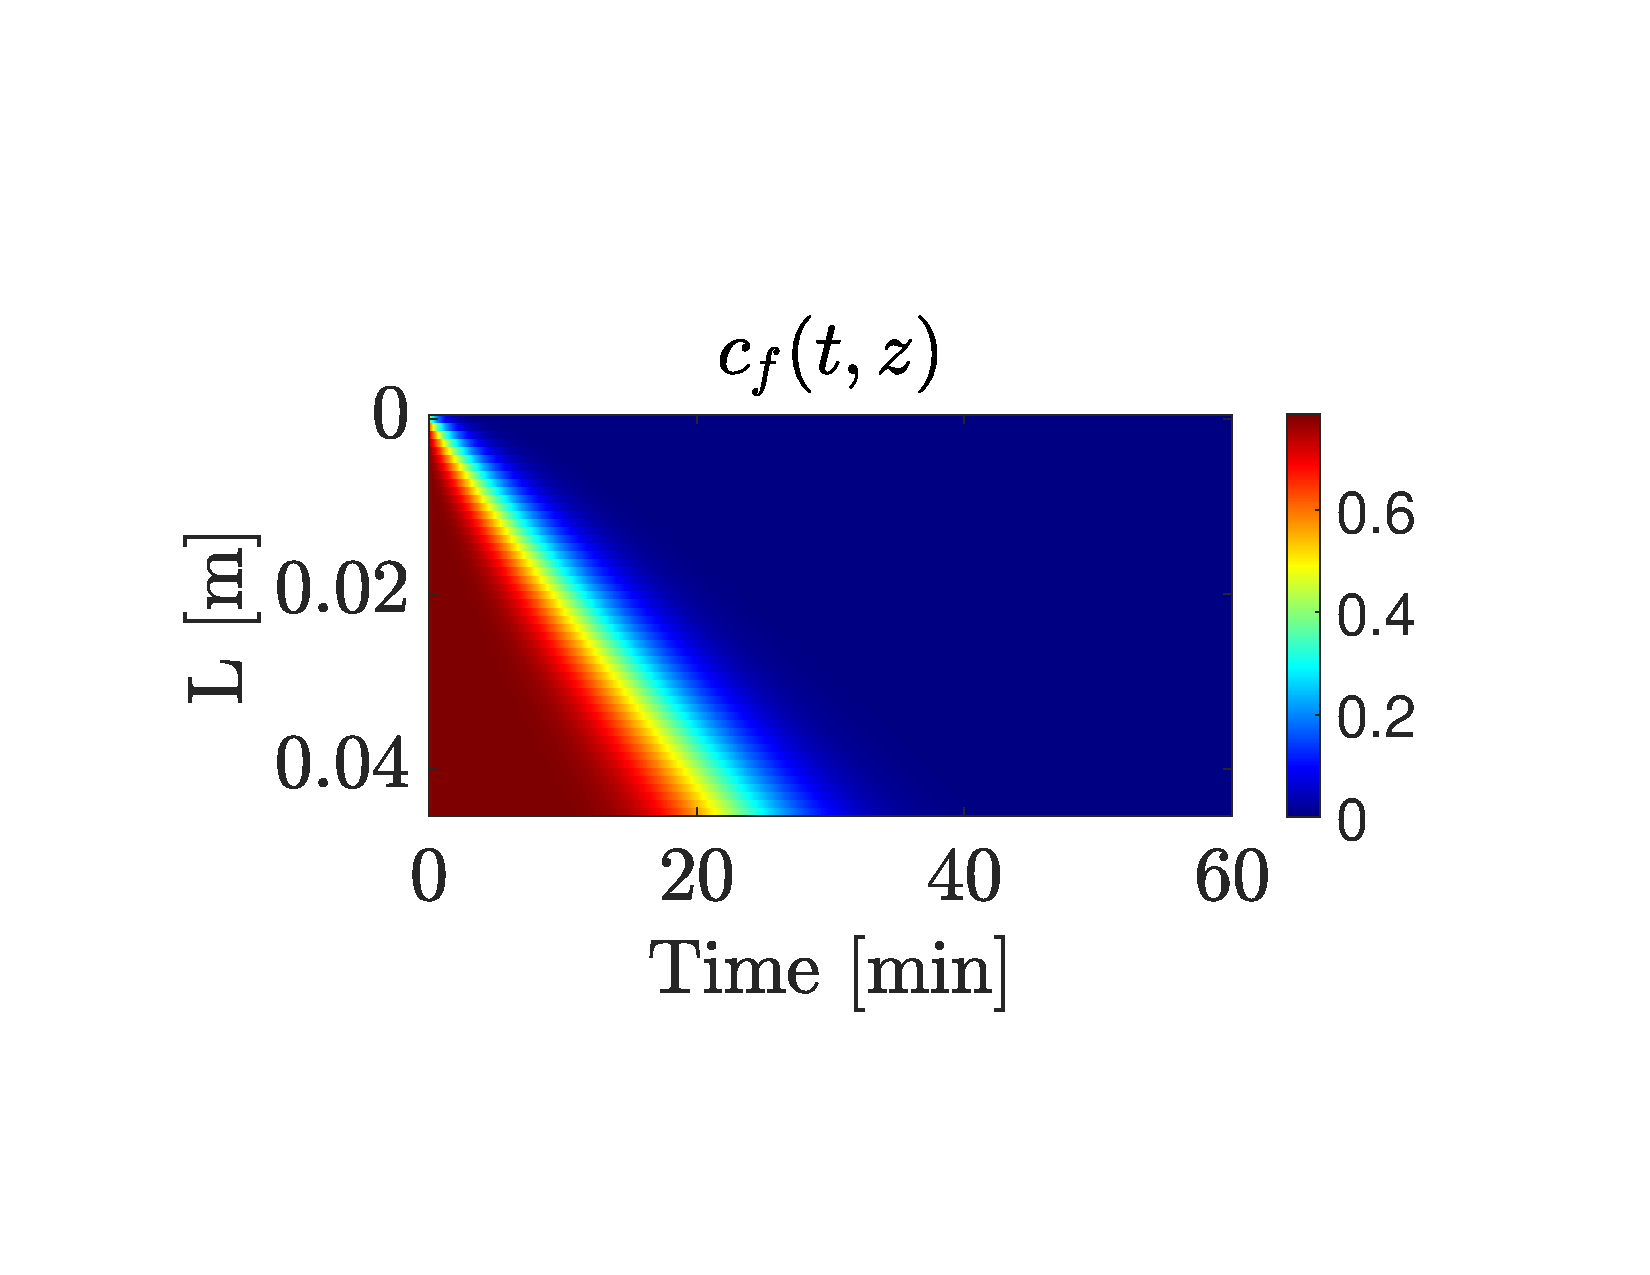
\includegraphics[trim = 3cm 4cm 2.5cm 4.3cm,clip,width=0.32\linewidth]{Figures/Sensitivity/ConcentrationLiquid.pdf} };
%				\node[yshift=3.3cm] at (Liq) {$c_f$};
				\node[xshift=-6.7cm,rotate=90] at (Liq) {${\color{white}F(t)}$};
				\node[inner sep=2pt] (Solid) at (12,0)
				{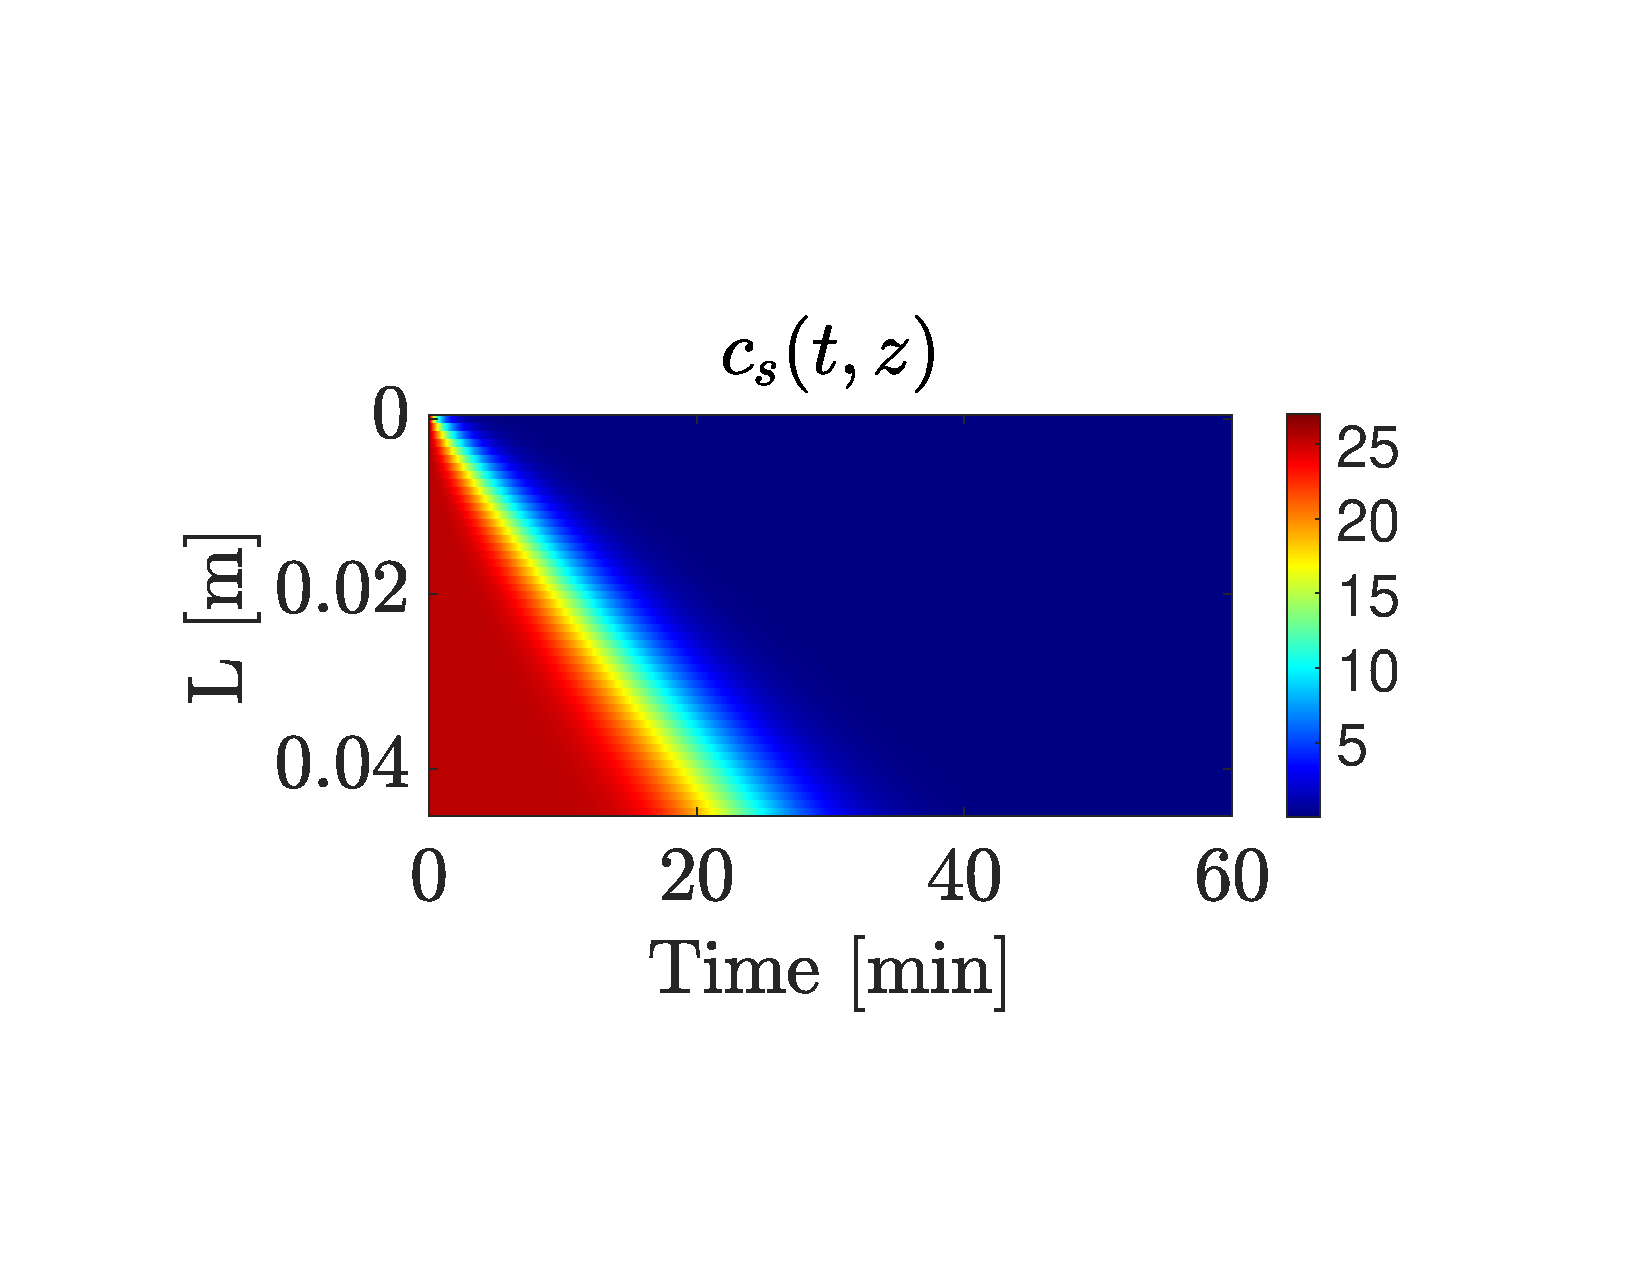
\includegraphics[trim = 3cm 4cm 2.5cm 4.3cm,clip,width=0.32\linewidth]{Figures/Sensitivity/ConcentrationSolid.pdf} };
%				\node[yshift=3.3cm] at (Solid) {$c_s$};
				\node[inner sep=2pt] (Yield) at (24,0)
				{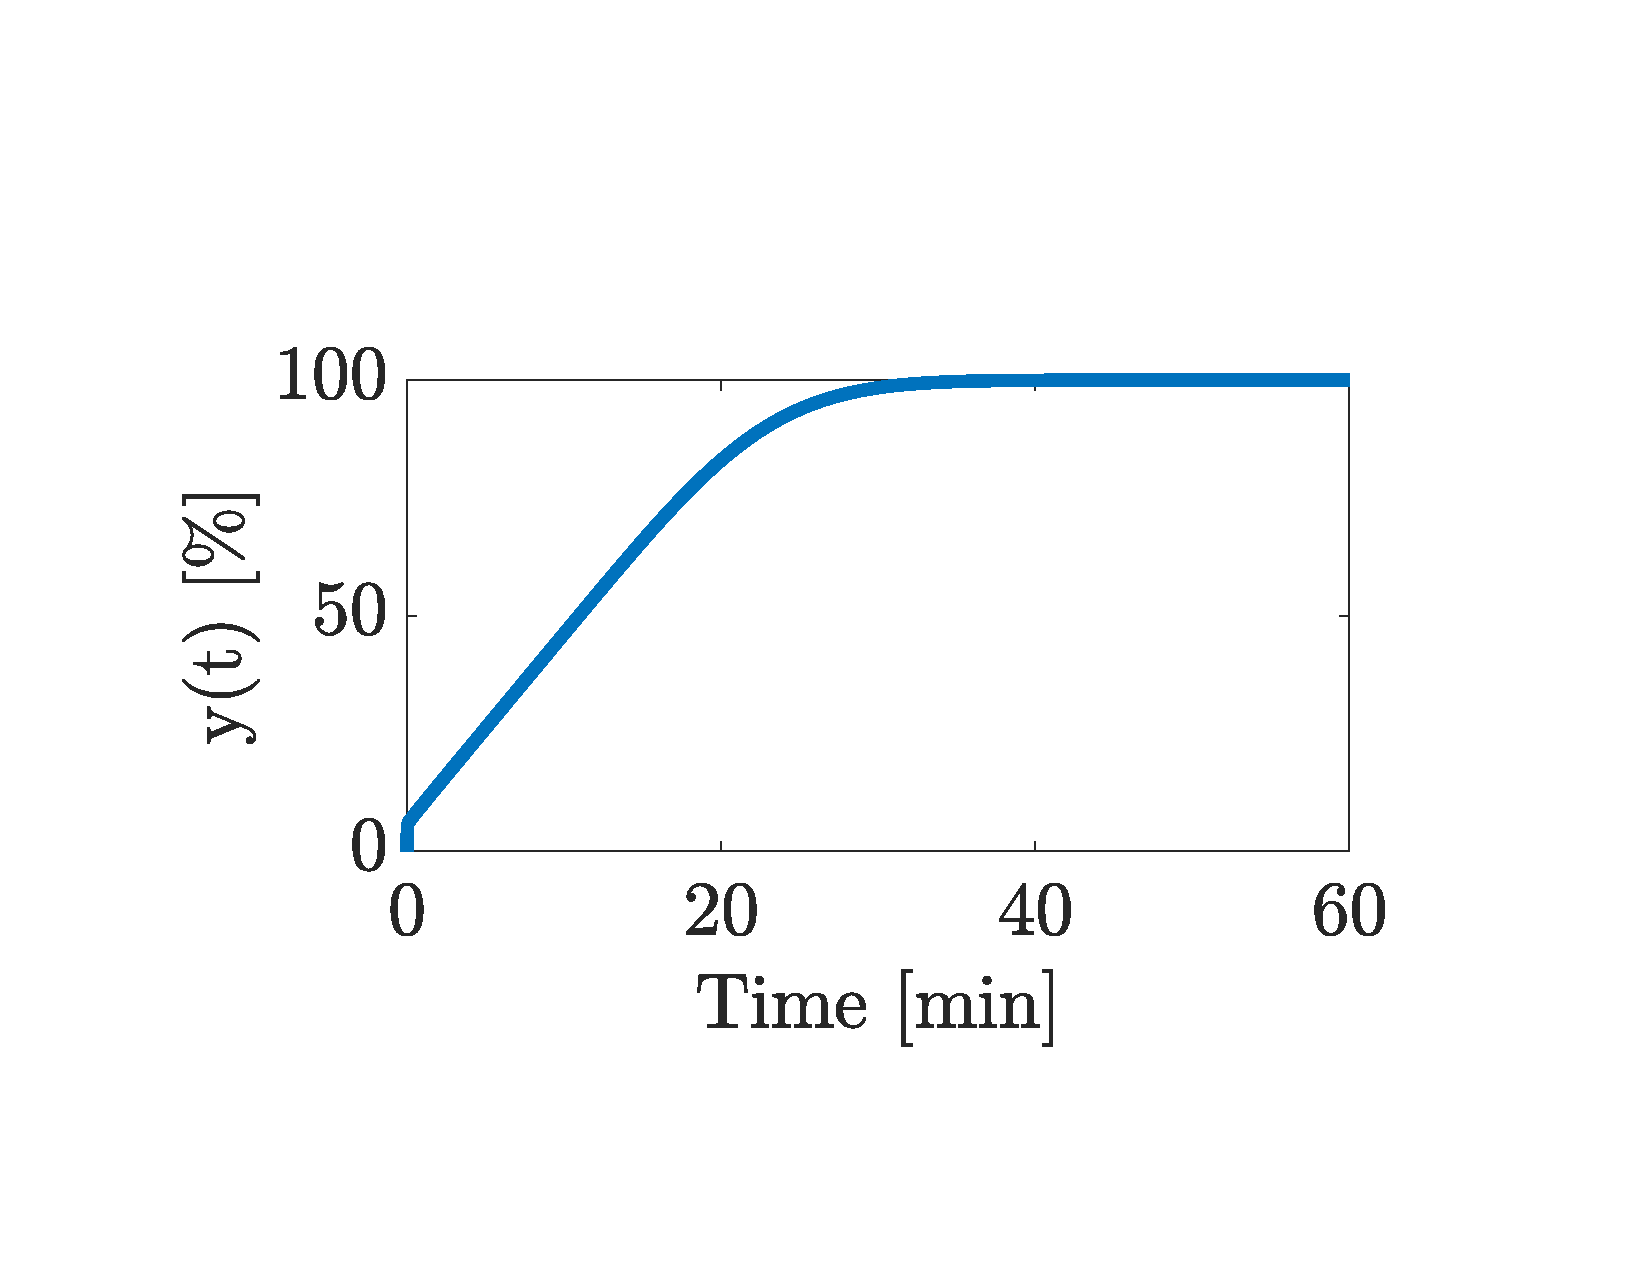
\includegraphics[trim = 3cm 4cm 2.5cm 4.3cm,clip,width=0.32\linewidth]{Figures/Sensitivity/Yield.pdf} };
%				\node[yshift=3.3cm] at (Yield) {$y(t)$};
%				\draw (-6.1,4.5) -- (-6.1,-2);
			\end{tikzpicture}
			
			\captionof{figure}{Solution of the process model}\label{Model_Solution}
			
			\vspace{0.5cm}
%			
			\hrule
			
			\vspace{1.0cm}
						
			We examine the effect of the operating conditions: ${\color{red}F}(t)$, ${\color{red}P}(t)$, ${\color{red}T_{Inlet}}(t)$ on the state variables: ${\color{blue}c_f}(t,z)$, ${\color{blue}c_s}(t,z)$ and on the observation function ${\color{blue}y}(t)$. The obtained results of the sensitivity analysis are presented in figure \ref{Sensitivty_Oper_Cond}
			
			
			\begin{tikzpicture} 
				\node[inner sep=2pt] (Liq1) at (0,0)
				{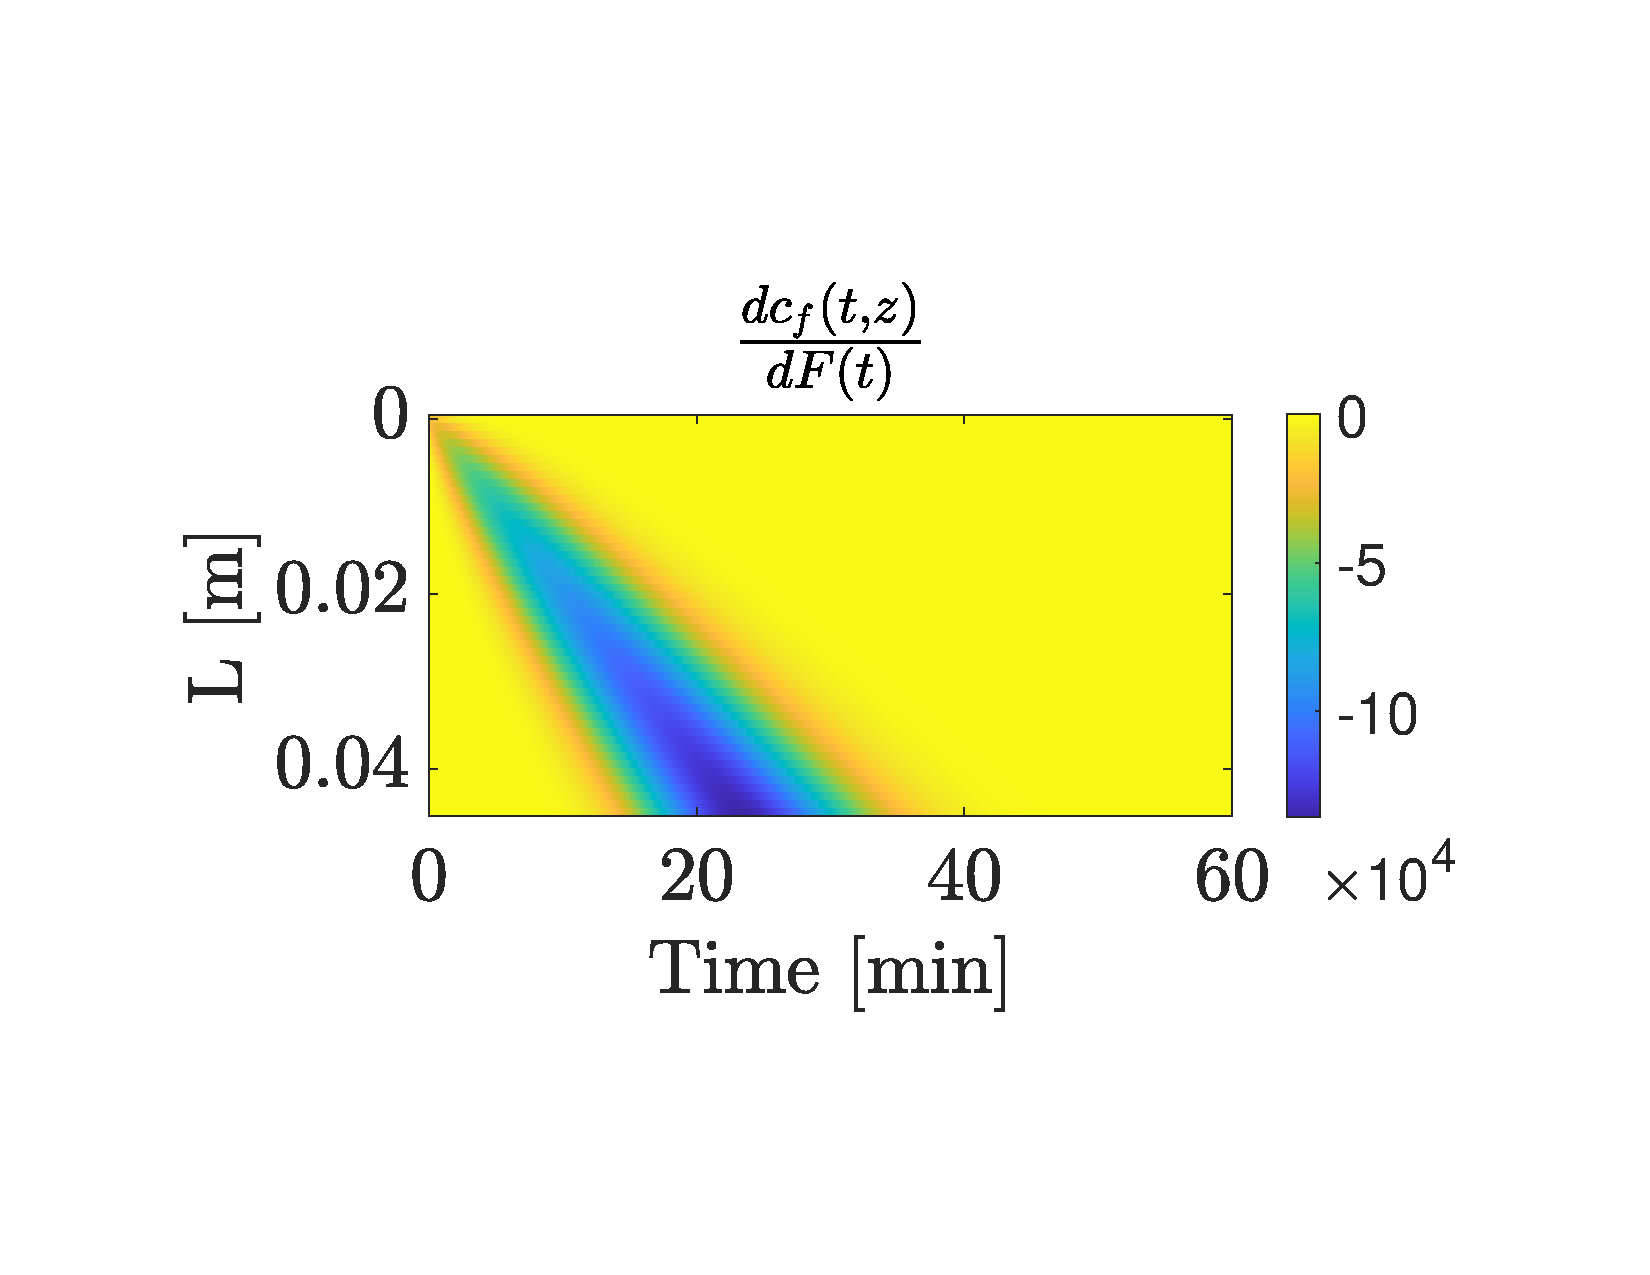
\includegraphics[trim = 3cm 4cm 2.5cm 4.3cm,clip,width=0.32\linewidth]{Figures/Sensitivity/Imagesc/2SS_RF.pdf} };
				\node[xshift=-6.7cm,rotate=90] at (Liq1) {${\color{red}F}(t)$};
				\node[inner sep=2pt] (Solid) at (12,0)
				{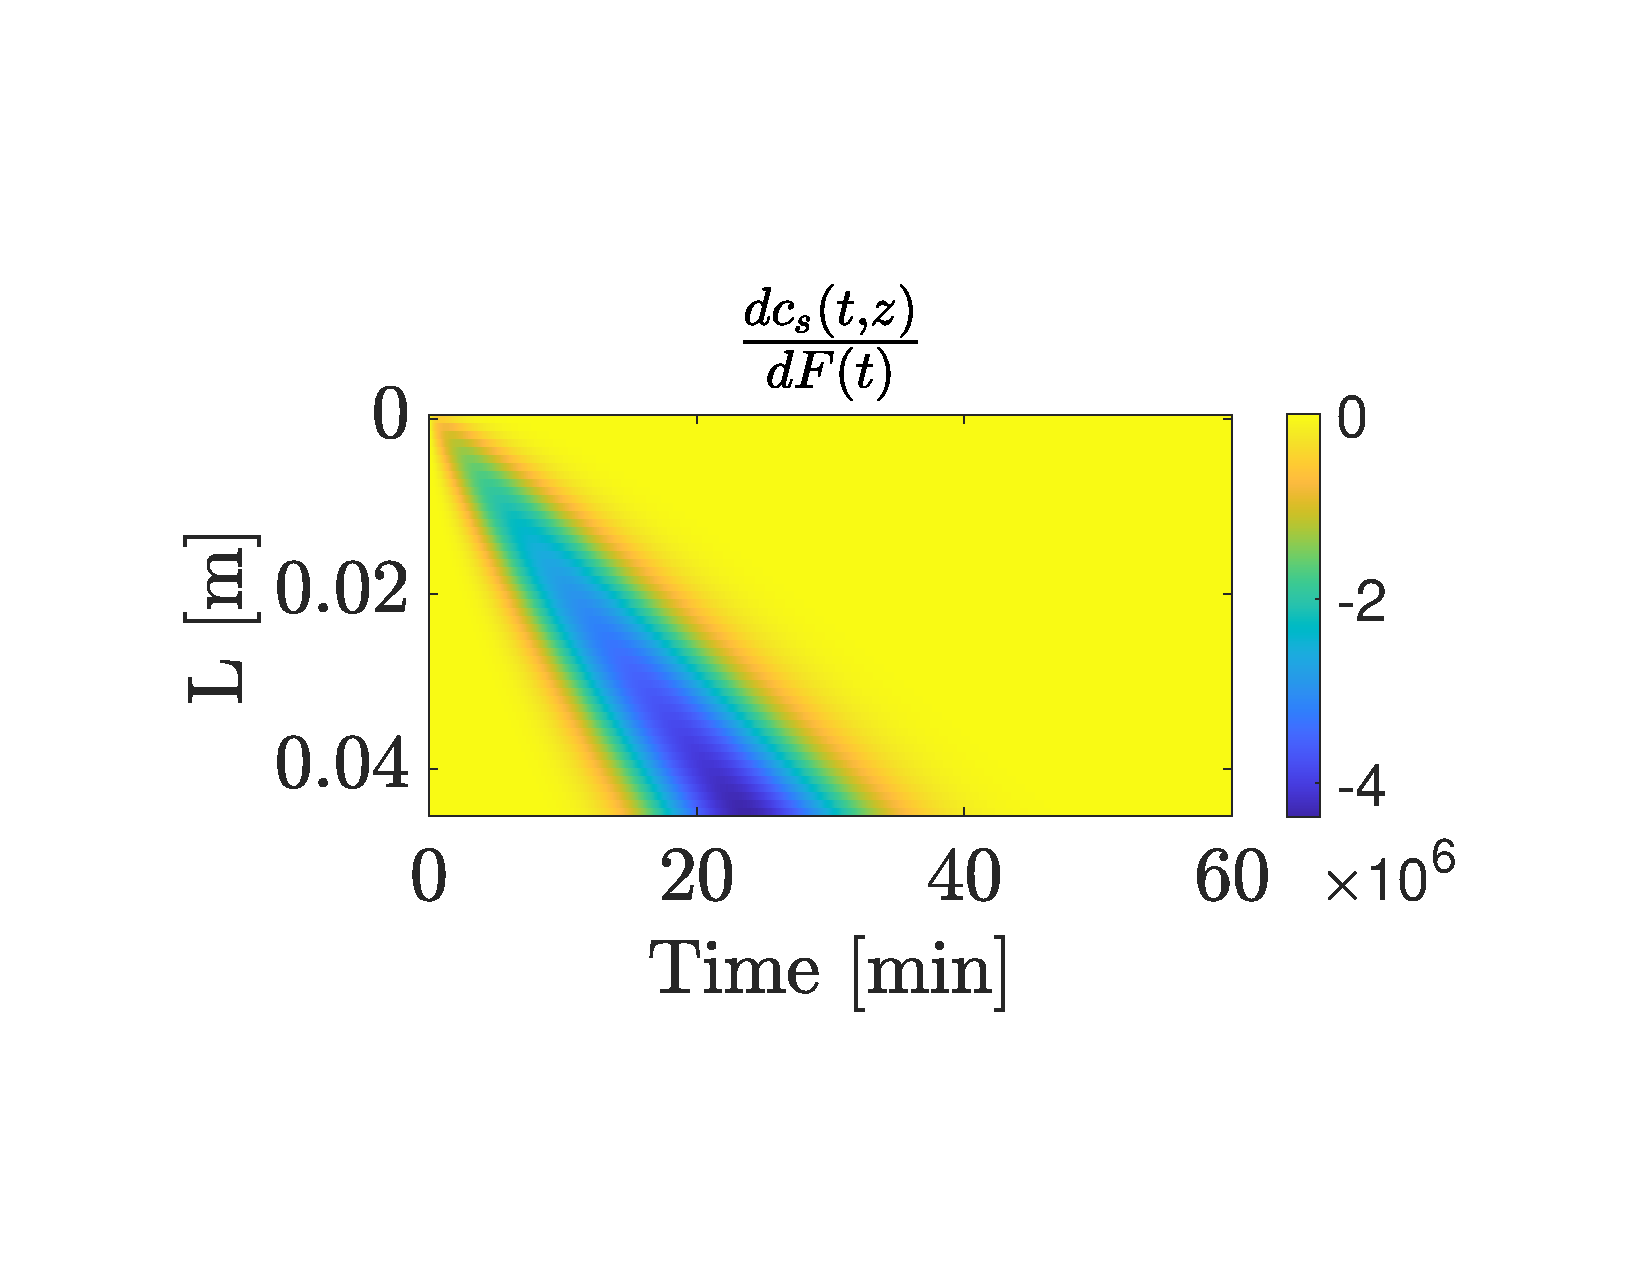
\includegraphics[trim = 3cm 4cm 2.5cm 4.3cm,clip,width=0.32\linewidth]{Figures/Sensitivity/Imagesc/3SS_RF.pdf} };
				\node[inner sep=2pt] (Yield) at (24,0)
				{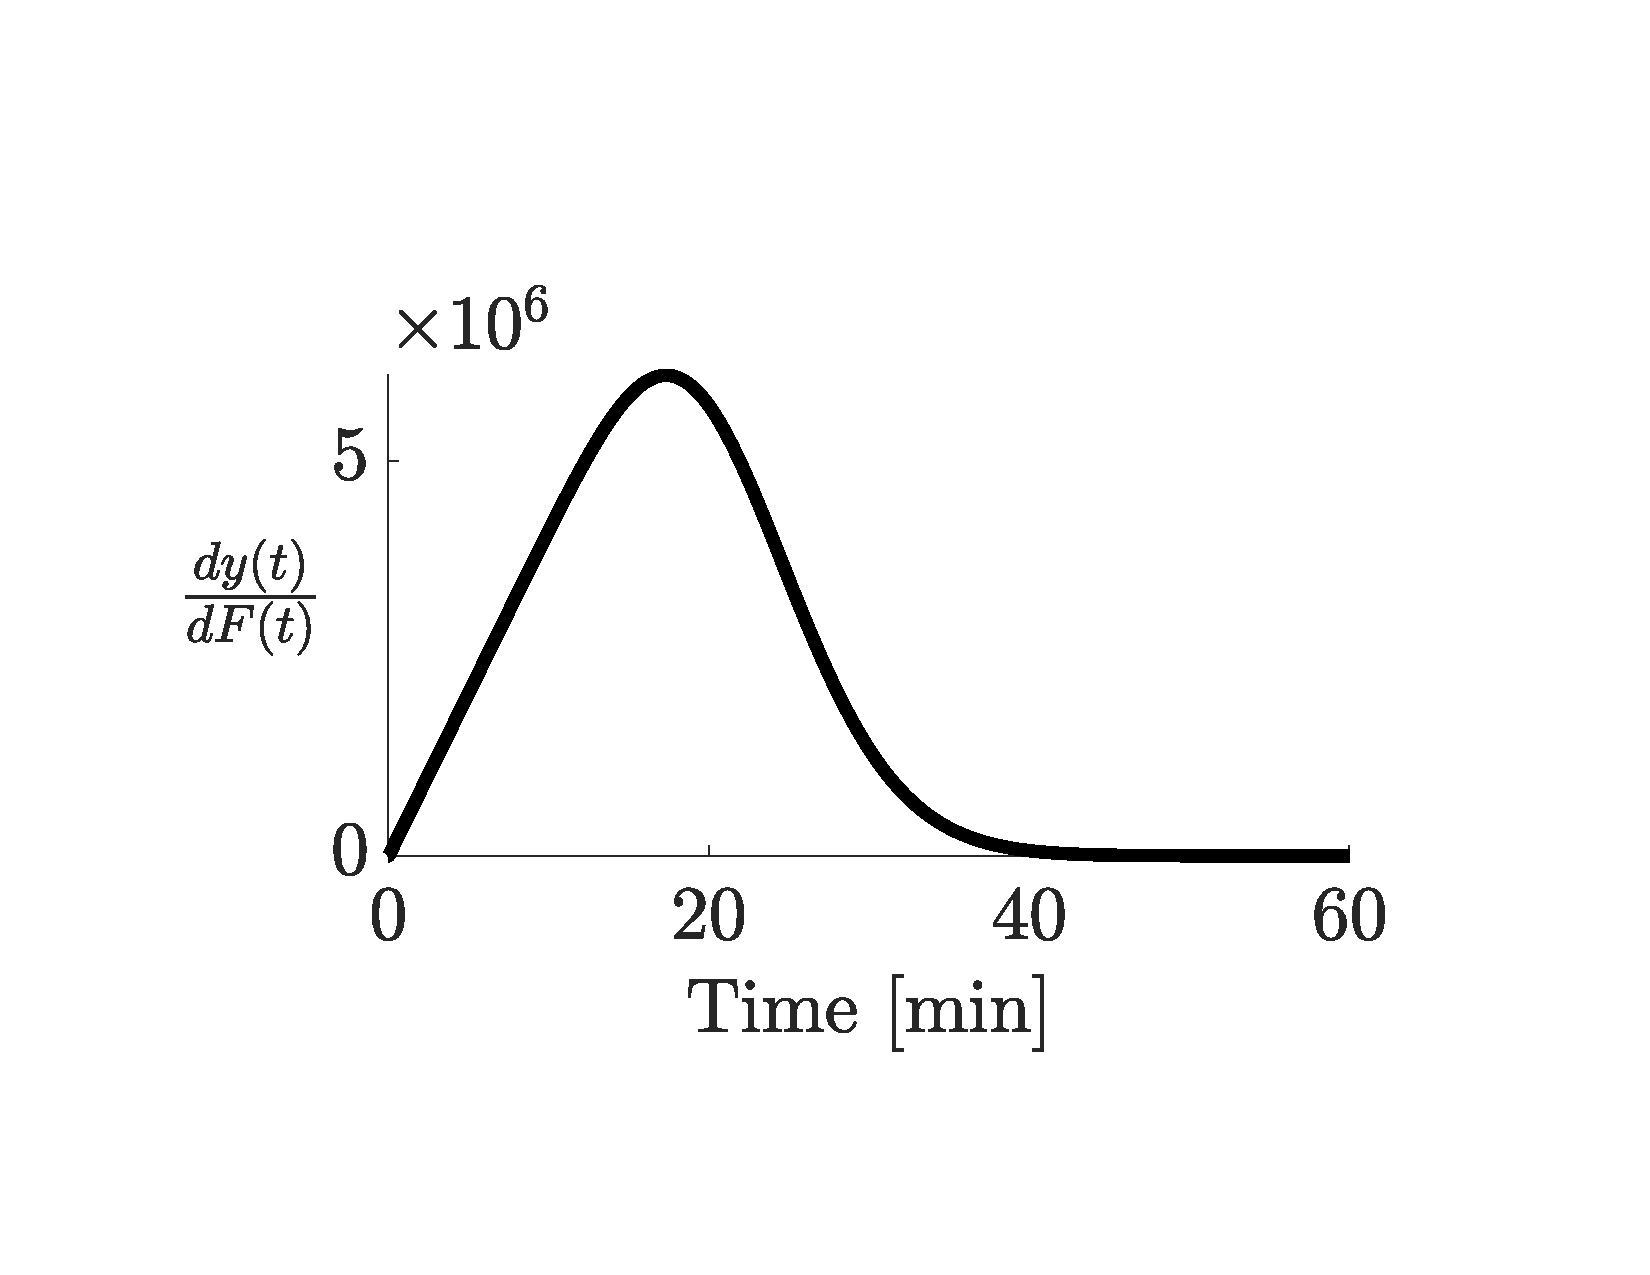
\includegraphics[trim = 3cm 3.5cm 2.5cm 4.3cm,clip,width=0.32\linewidth]{Figures/Sensitivity/Imagesc/1SS_RF.pdf} };
				\draw (-6.1,2.3) -- (-6.1,-16);
				
				\node[inner sep=2pt] (Liq2) at (0,-7)
				{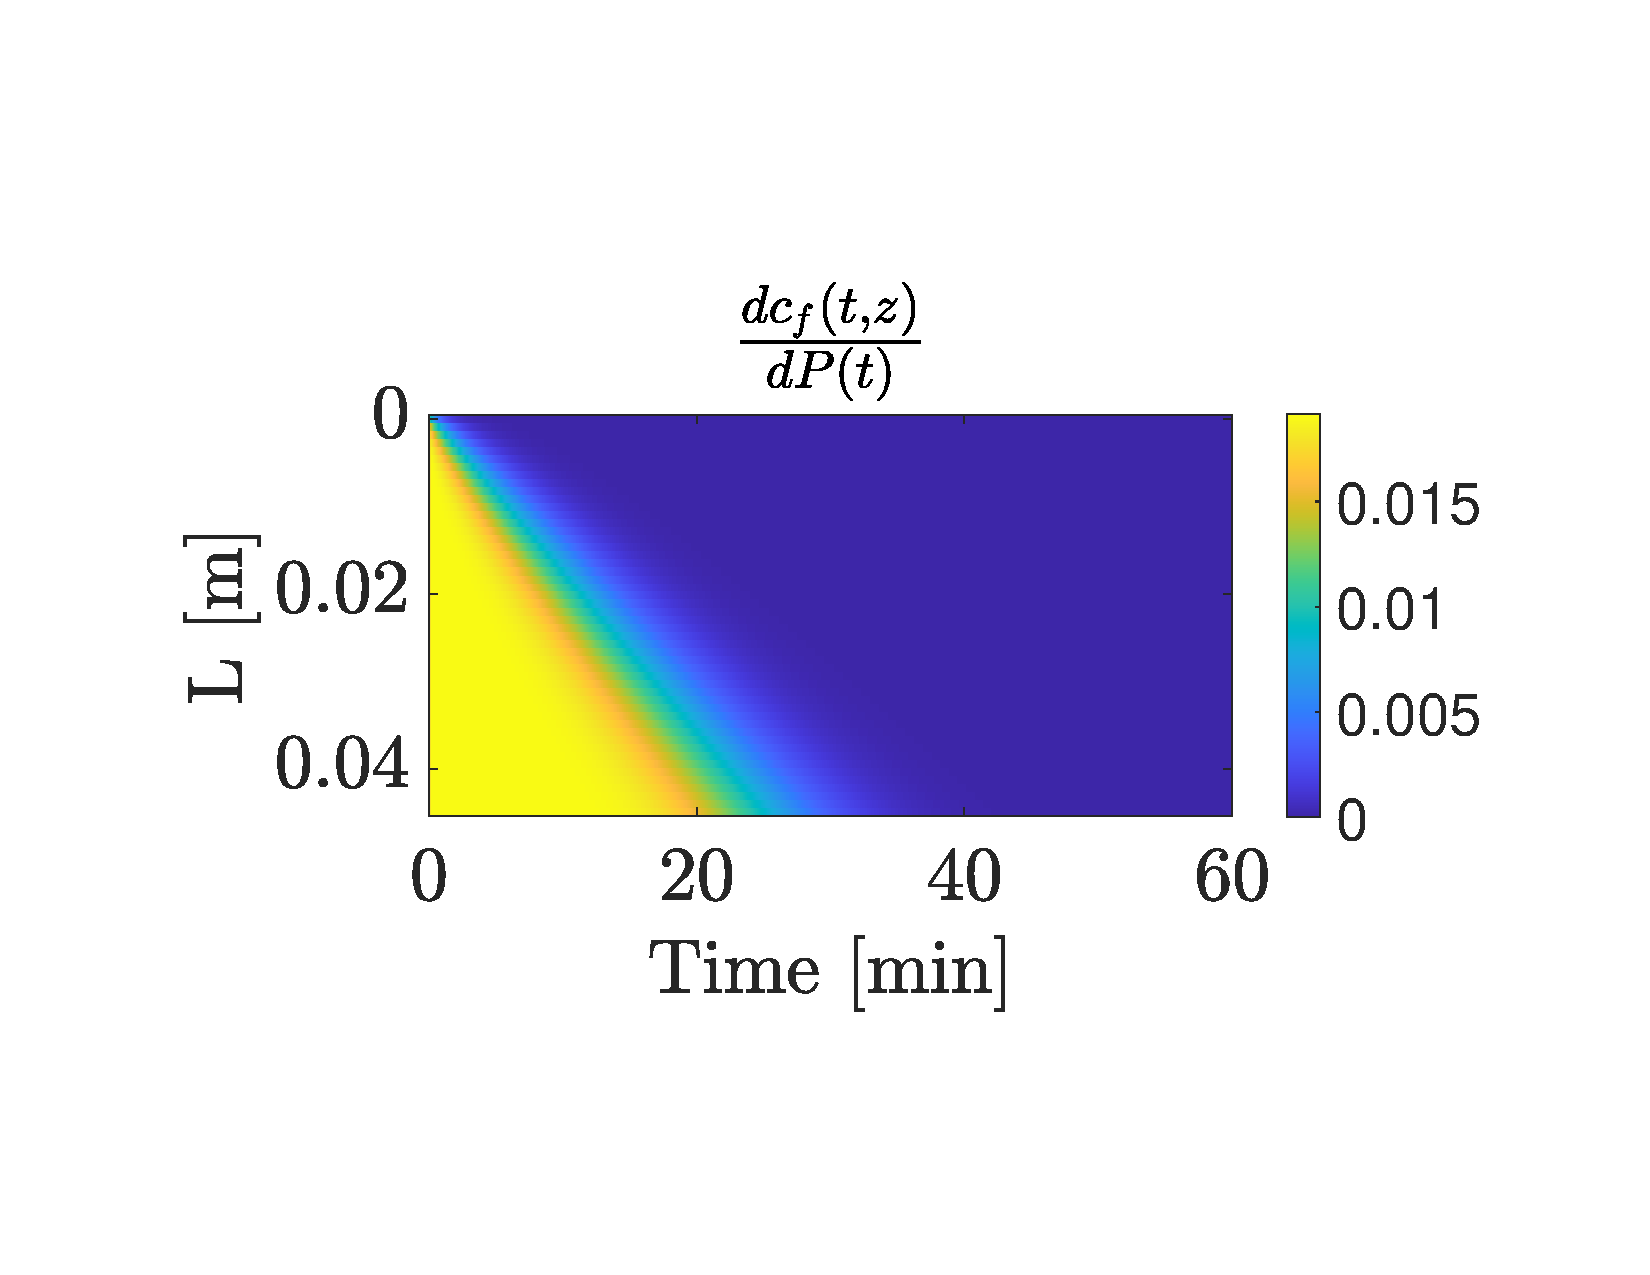
\includegraphics[trim = 3cm 4cm 2.5cm 4.3cm,clip,width=0.32\linewidth]{Figures/Sensitivity/Imagesc/2SS_RP.pdf} };
				\node[xshift=-6.7cm,rotate=90] at (Liq2) {${\color{red}P}(t)$};
				\node[inner sep=2pt] (Solid) at (12,-7)
				{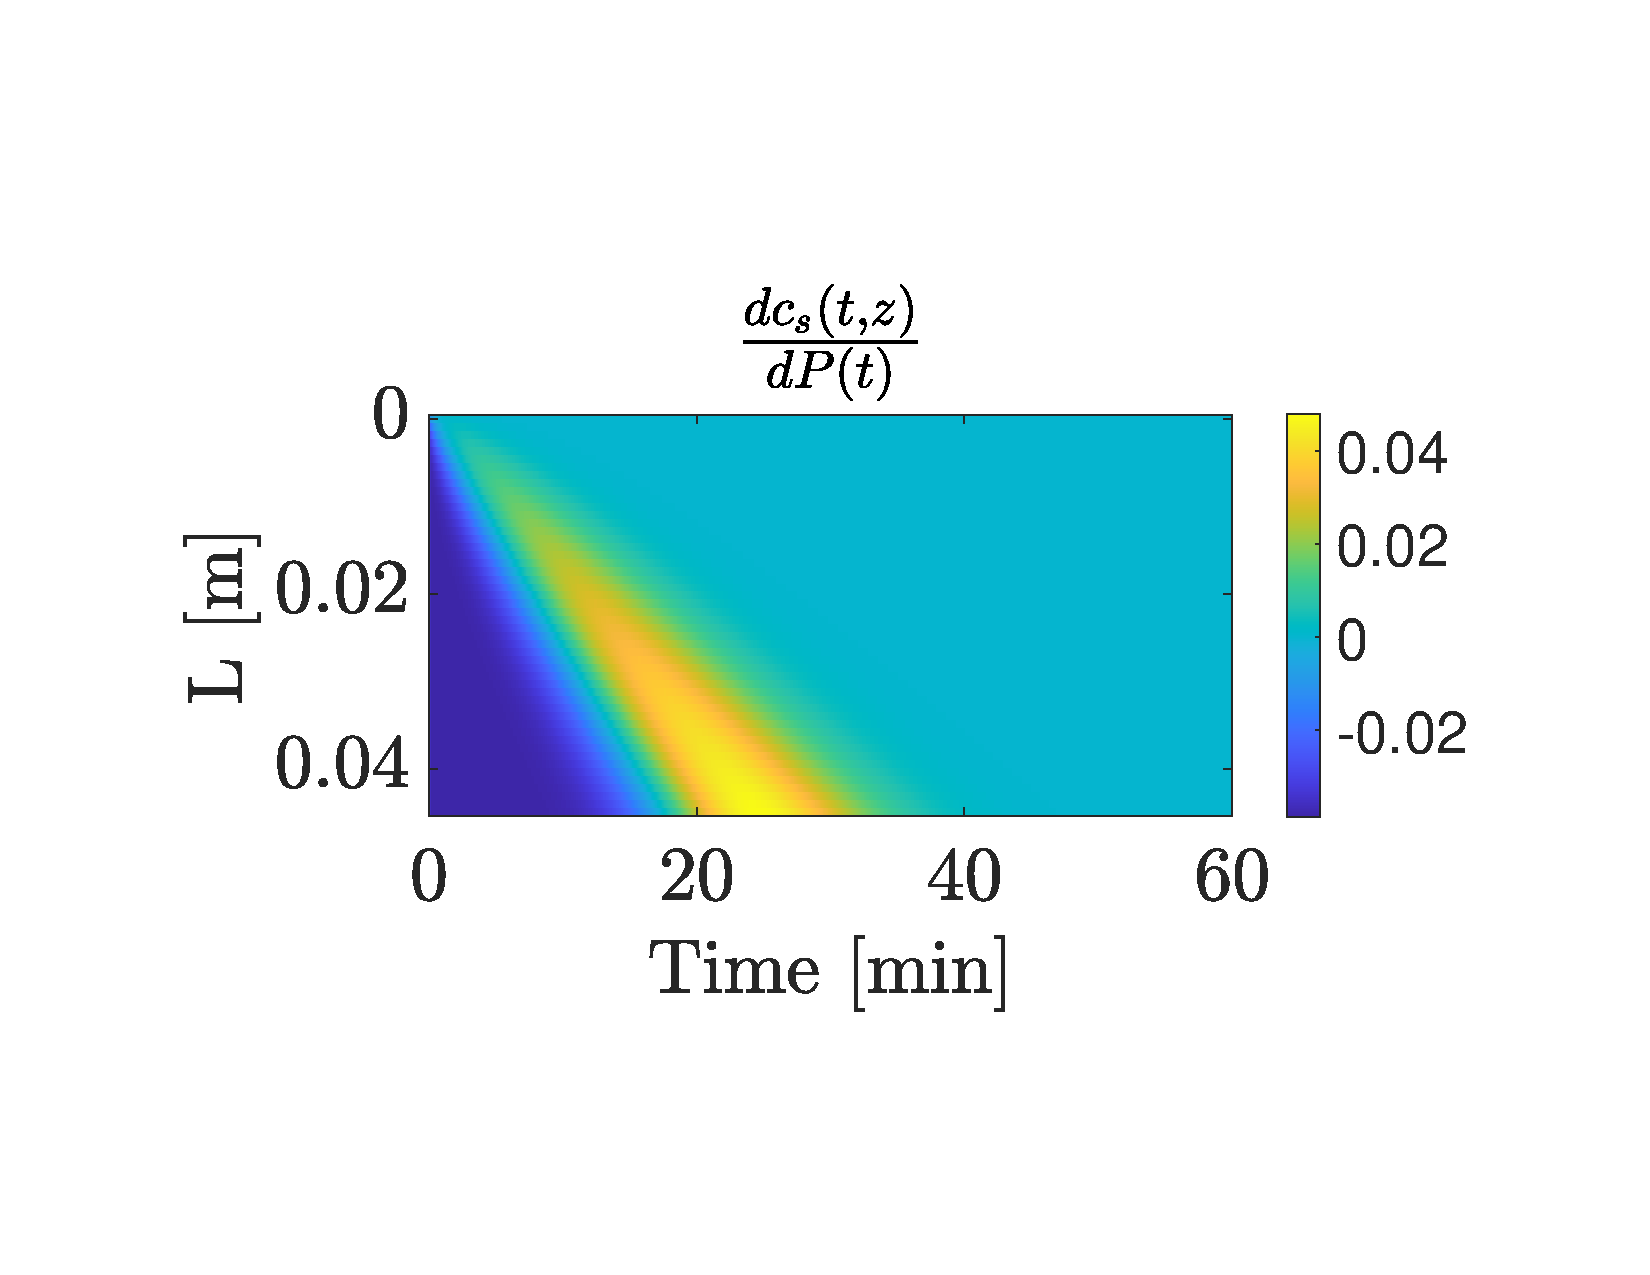
\includegraphics[trim = 3cm 4cm 2.5cm 4.3cm,clip,width=0.32\linewidth]{Figures/Sensitivity/Imagesc/3SS_RP.pdf} };
				\node[inner sep=2pt] (Yield) at (24,-7)
				{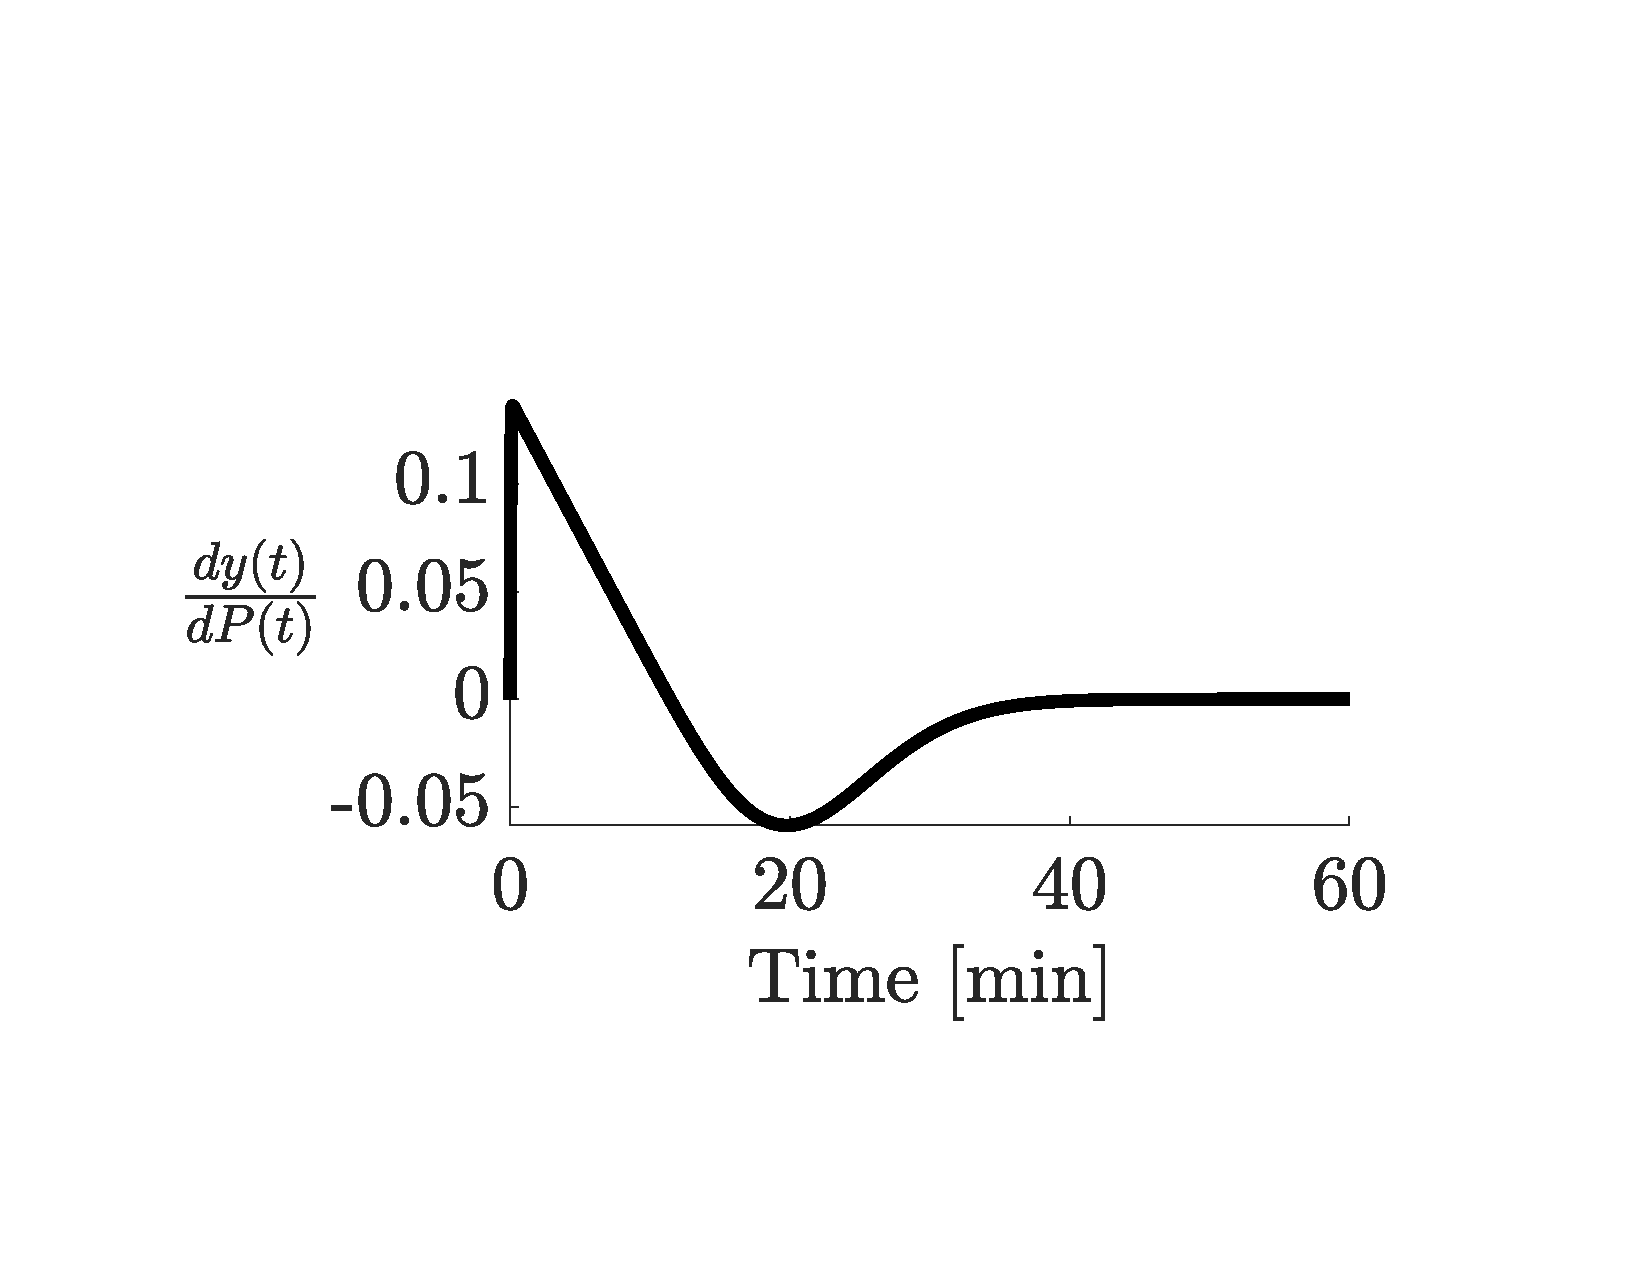
\includegraphics[trim = 3cm 4cm 2.5cm 4.3cm,clip,width=0.32\linewidth]{Figures/Sensitivity/Imagesc/1SS_RP.pdf} };

				\node[inner sep=2pt] (Liq3) at (0,-14)
				{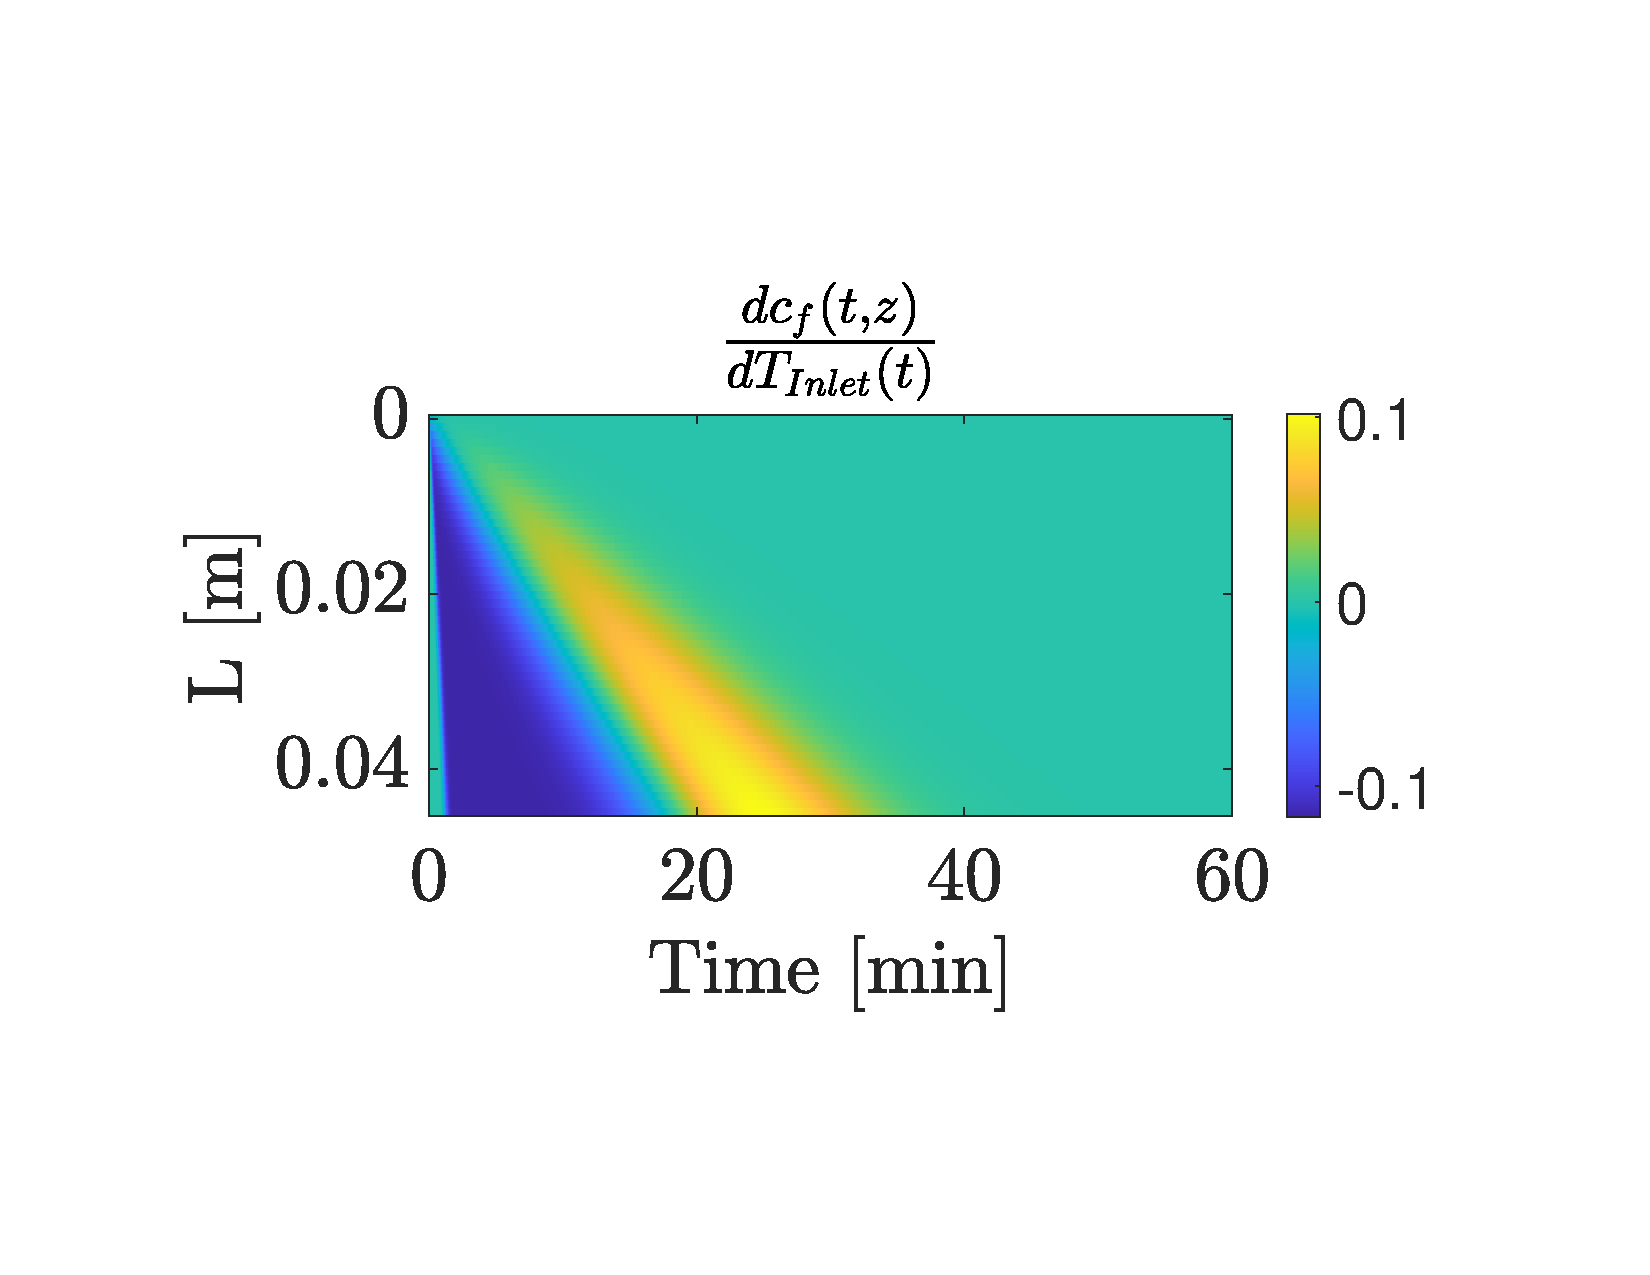
\includegraphics[trim = 3cm 4cm 2.5cm 4.3cm,clip,width=0.32\linewidth]{Figures/Sensitivity/Imagesc/2SS_RT.pdf} };
				\node[xshift=-6.7cm,rotate=90] at (Liq3) {${\color{red}T_{Inlet}}(t)$};
				\node[inner sep=2pt] (Solid) at (12,-14)
				{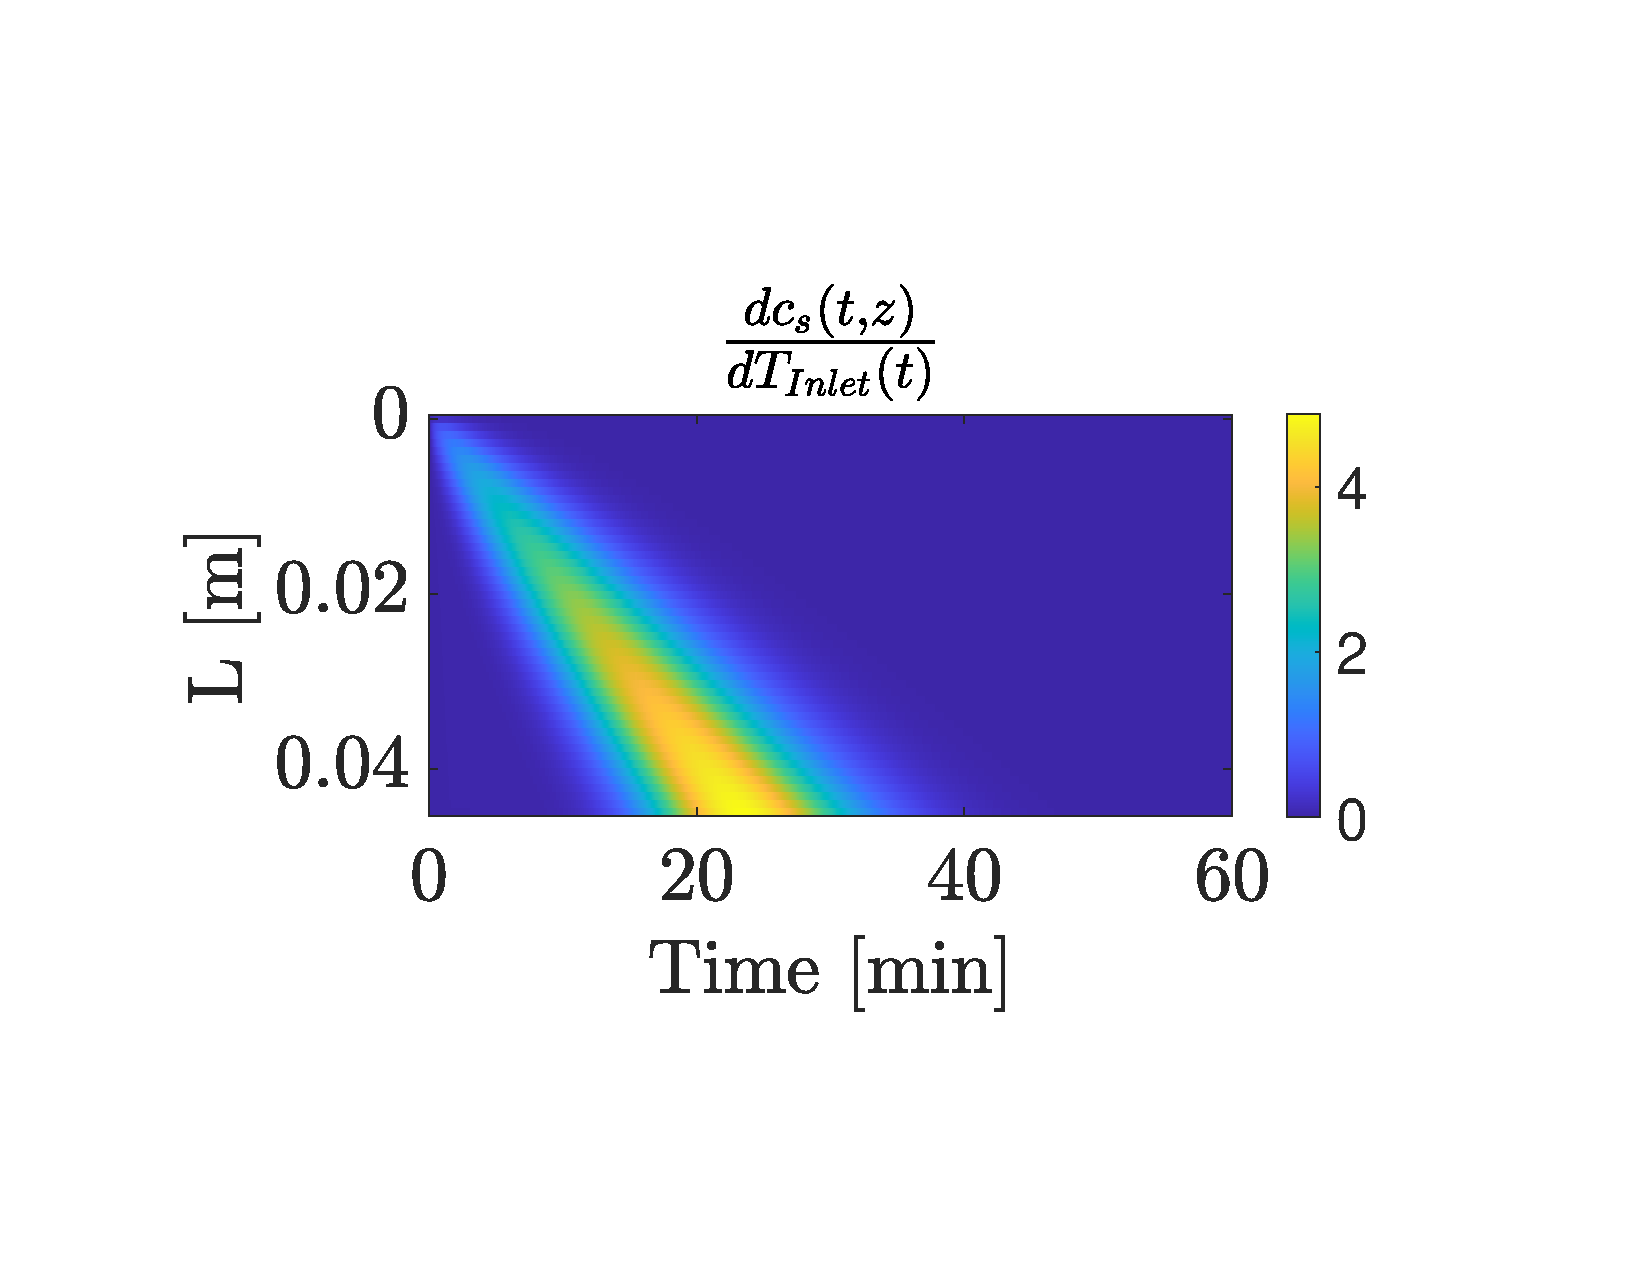
\includegraphics[trim = 3cm 4cm 2.5cm 4.3cm,clip,width=0.32\linewidth]{Figures/Sensitivity/Imagesc/3SS_RT.pdf} };
				\node[inner sep=2pt] (Yield) at (24,-14)
				{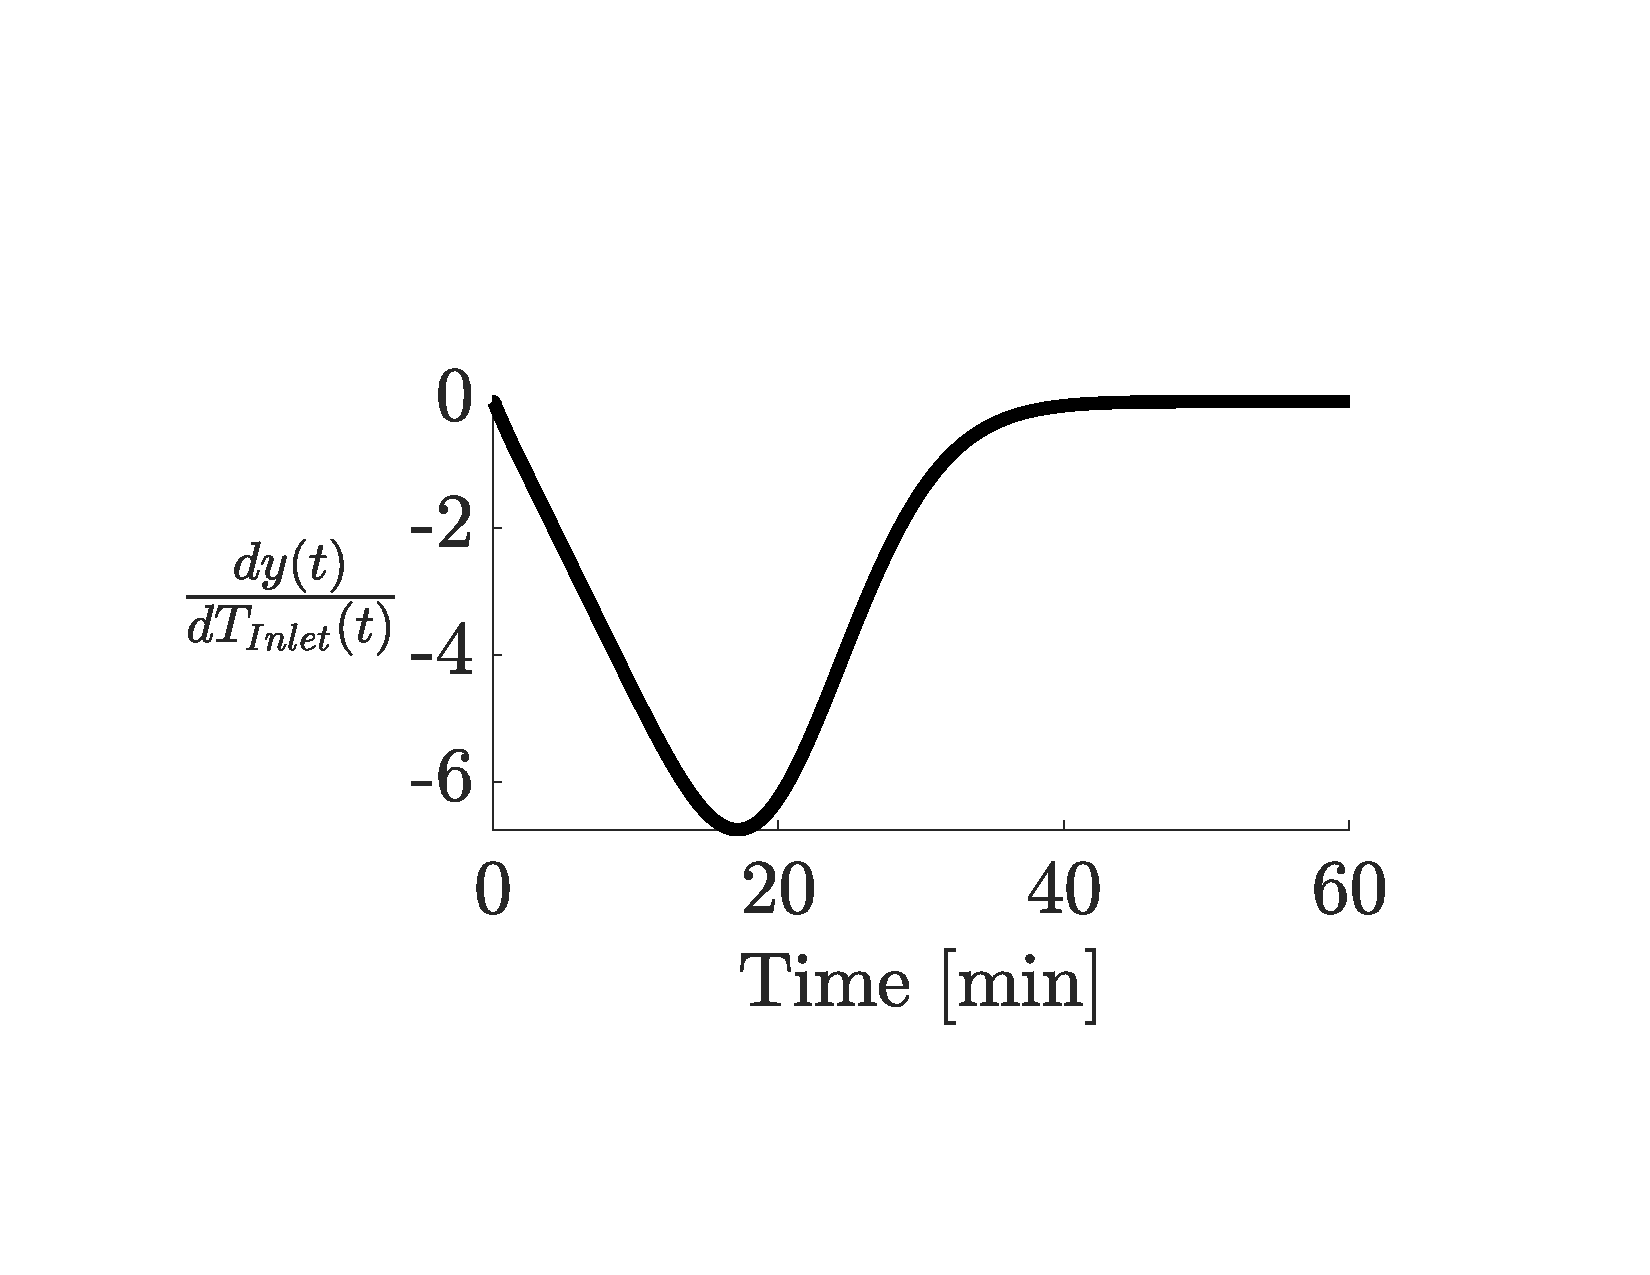
\includegraphics[trim = 3cm 4cm 2.5cm 4.3cm,clip,width=0.32\linewidth]{Figures/Sensitivity/Imagesc/1SS_RT.pdf} };
			\end{tikzpicture}
			\captionof{figure}{Results of the sensitivity analysis with respect to operating conditions} \label{Sensitivty_Oper_Cond}
			
			\vspace{0.5cm}
		
			\hrule
			
			\vspace{1.0cm}
			
			Similarly, we examine the effect of selected parameters: ${\color{magenta}\epsilon}$ and ${\color{magenta}l}$ on state variables: ${\color{blue}c_f}(t,z)$, ${\color{blue}c_s}(t,z)$ and on the observation function ${\color{blue}y}(t)$. The obtained results of the sensitivity analysis are presented in figure \ref{Sensitivty_Parameters}
			
			\begin{tikzpicture}
				\node[inner sep=2pt] (Liq1) at (0,0)
				{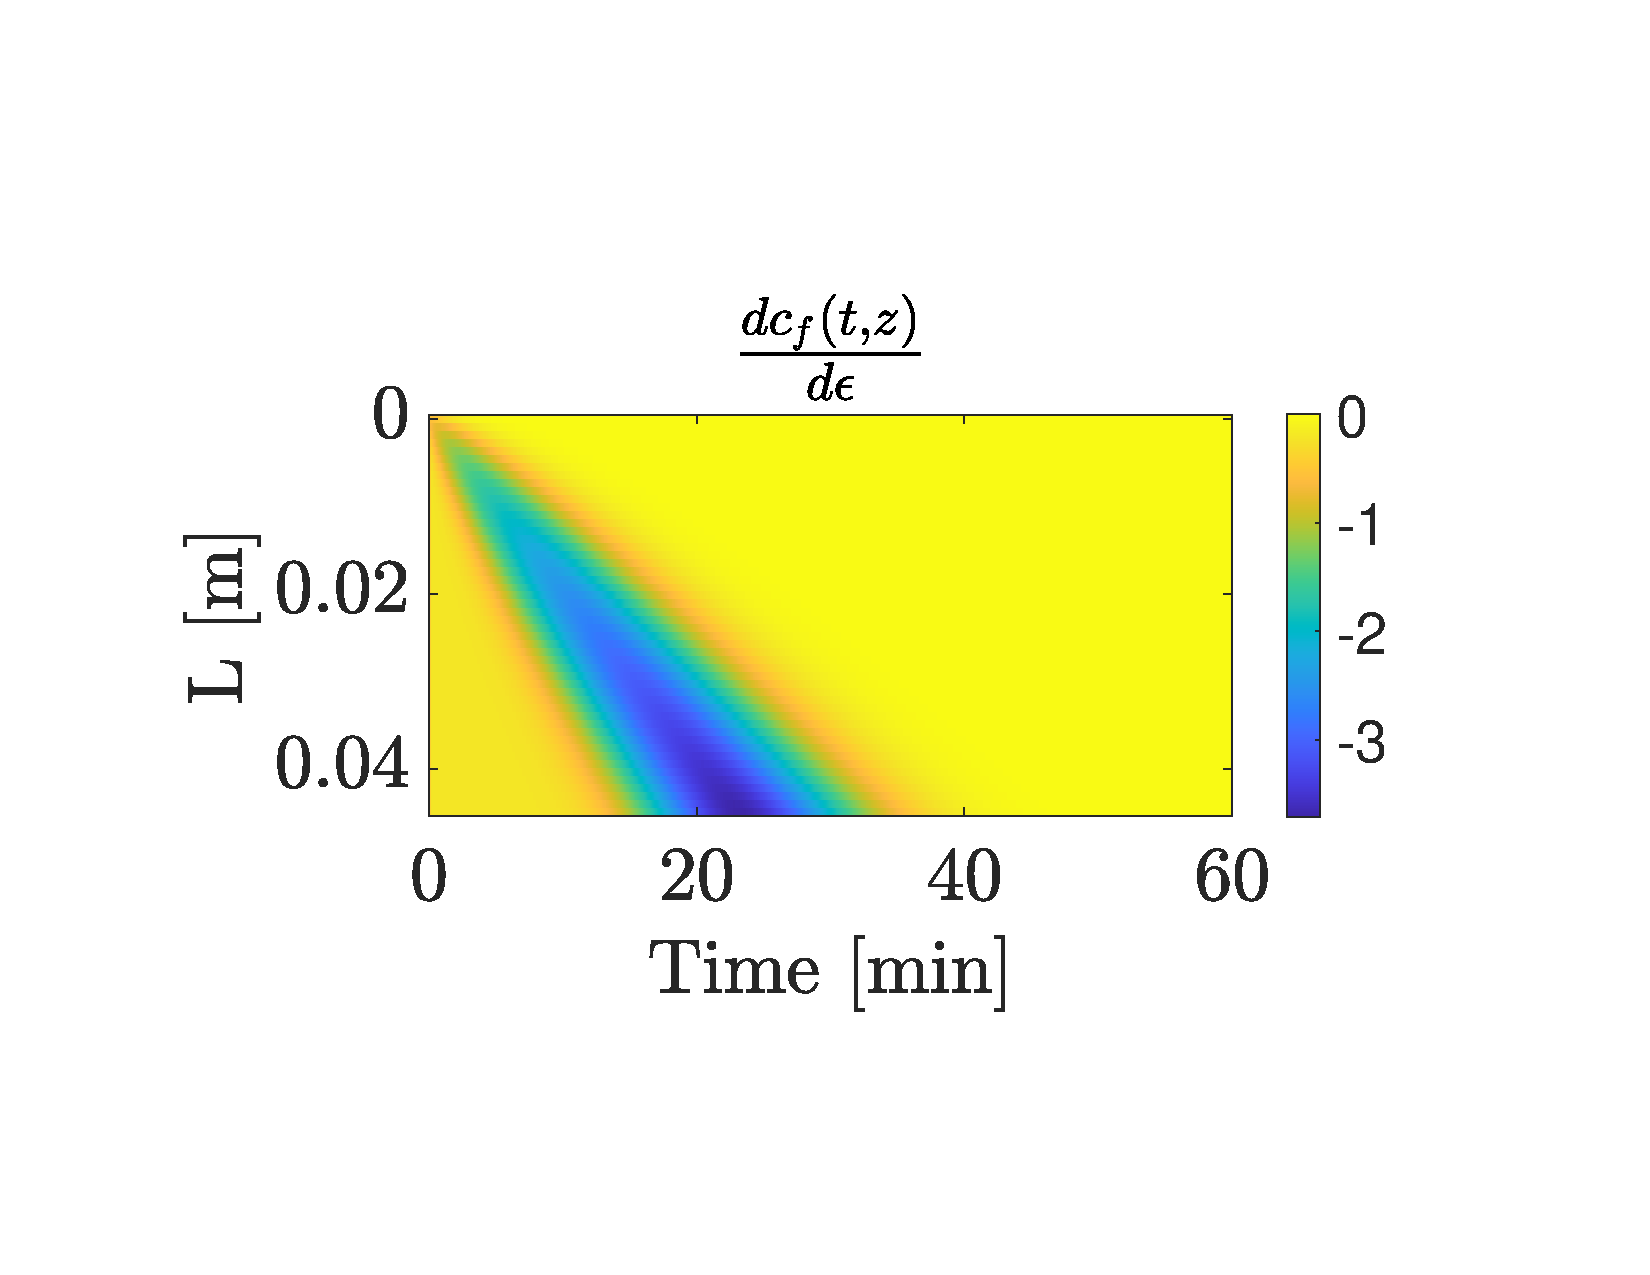
\includegraphics[trim = 3cm 4cm 2.5cm 4.3cm,clip,width=0.32\linewidth]{Figures/Sensitivity/Imagesc/2SS_Repsi.pdf} };
				\node[xshift=-6.7cm,rotate=90] at (Liq1) {${\color{magenta}\epsilon}{\color{white}(t)}$};
				\node[inner sep=2pt] (Solid) at (12,0)
				{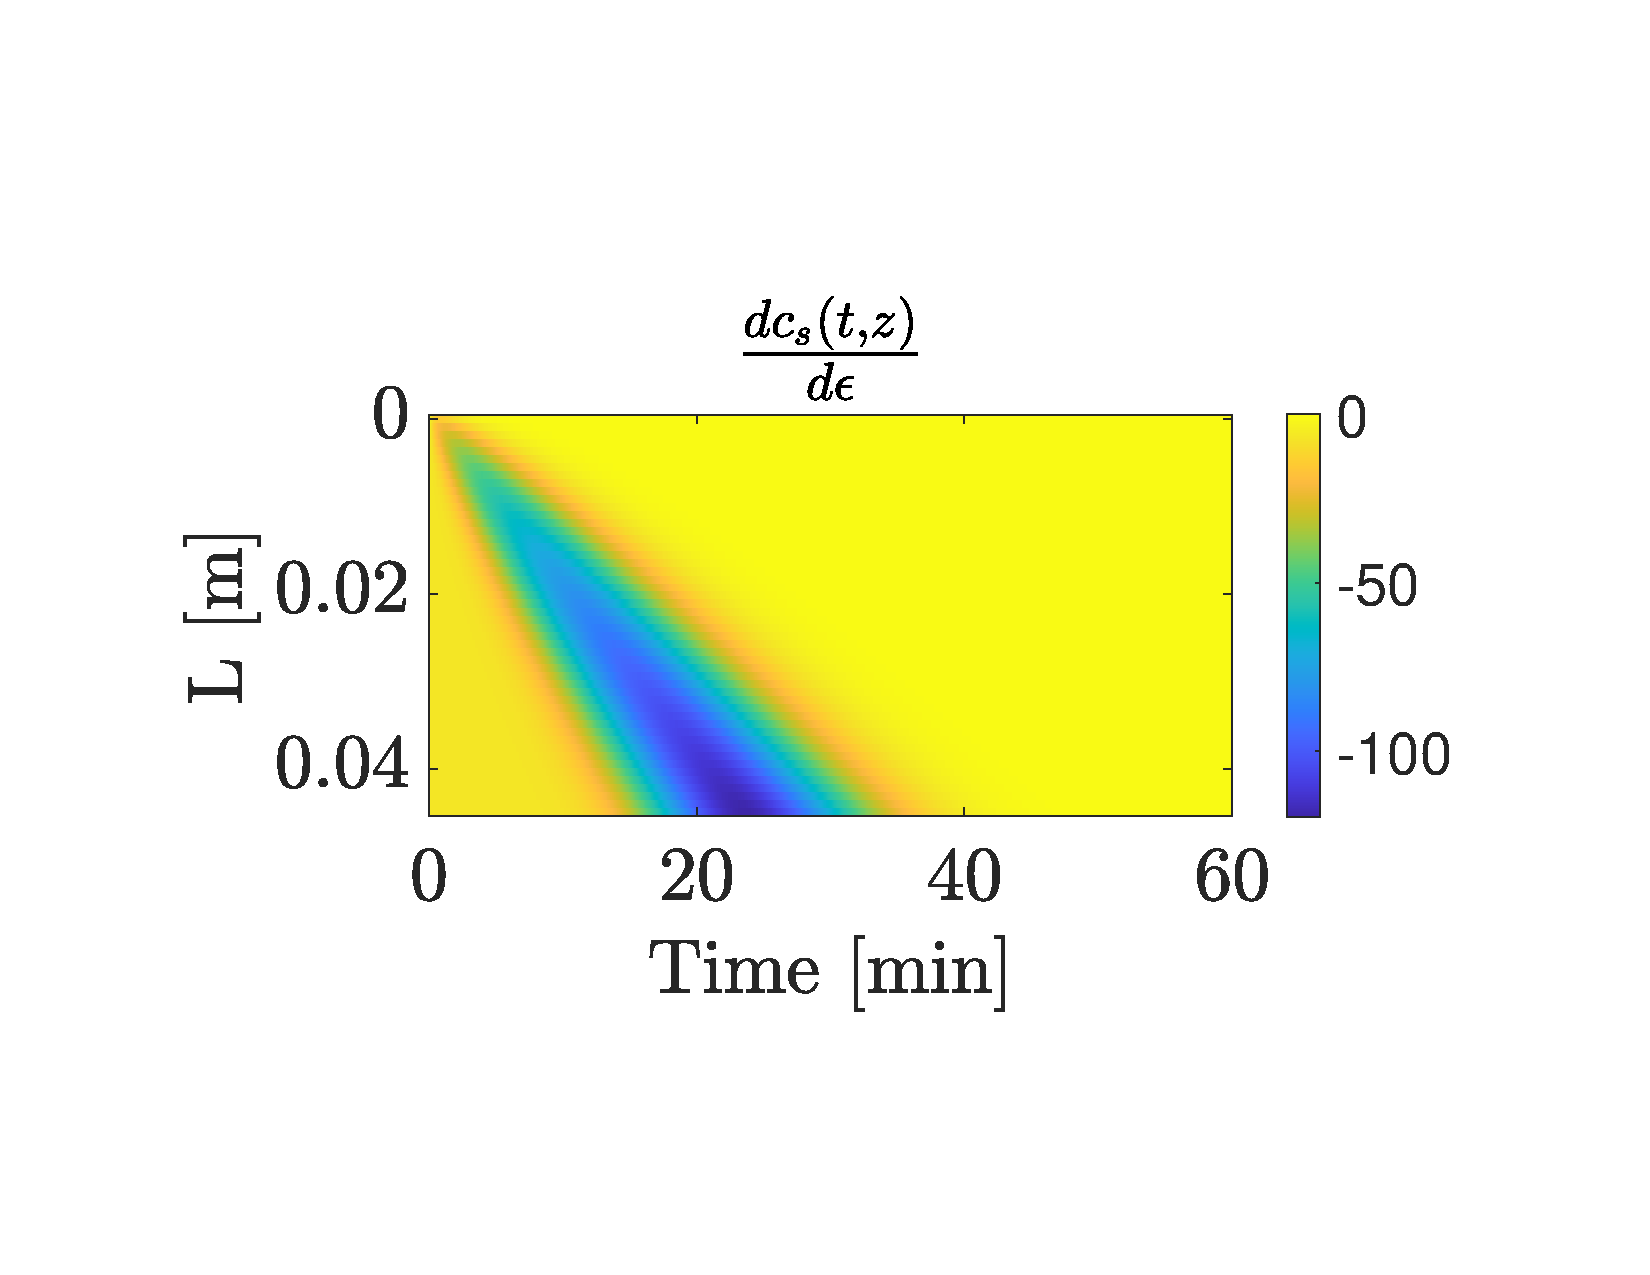
\includegraphics[trim = 3cm 4cm 2.5cm 4.3cm,clip,width=0.32\linewidth]{Figures/Sensitivity/Imagesc/3SS_Repsi.pdf} };
				\node[inner sep=2pt] (Yield) at (24,0)
				{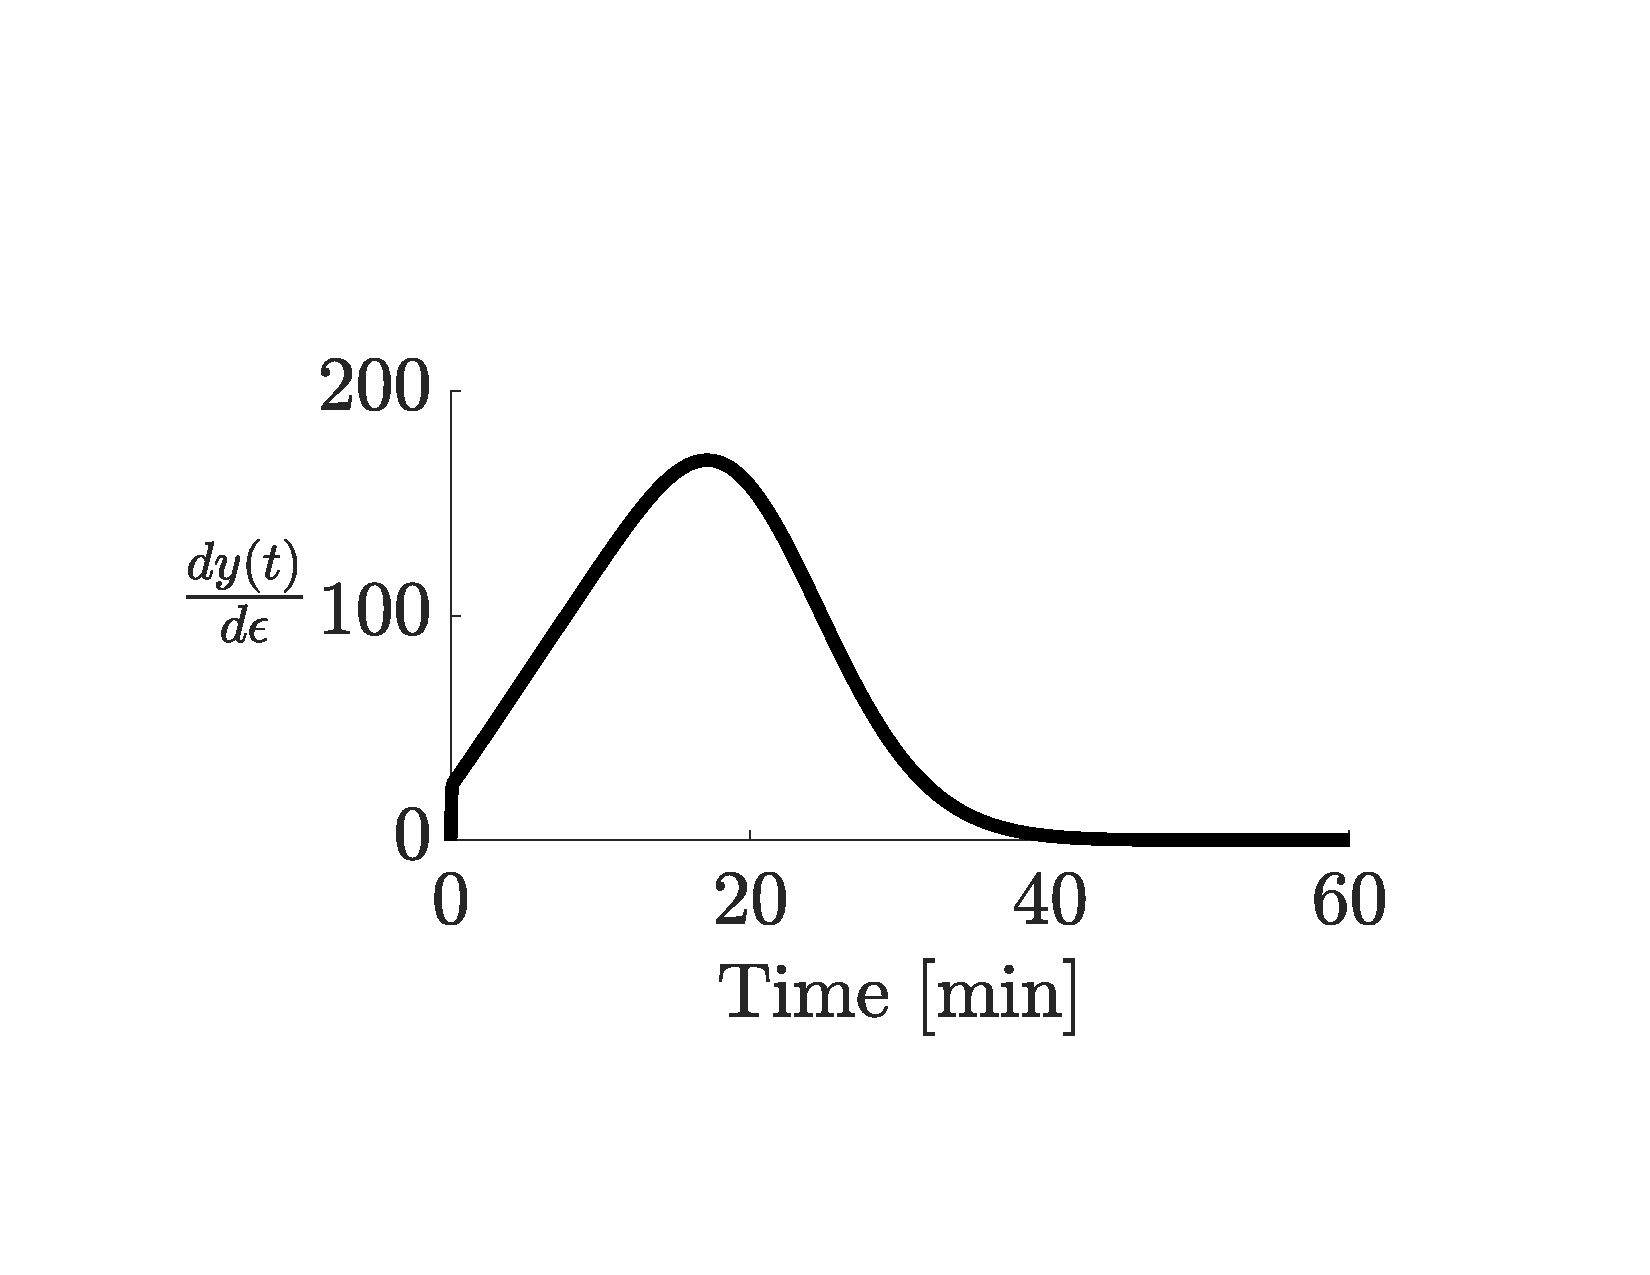
\includegraphics[trim = 3cm 4cm 2.5cm 4.3cm,clip,width=0.32\linewidth]{Figures/Sensitivity/Imagesc/1SS_Repsi.pdf} };
				\draw (-6.1,2.3) -- (-6.1,-9);
				
				\node[inner sep=2pt] (Liq2) at (0,-7)
				{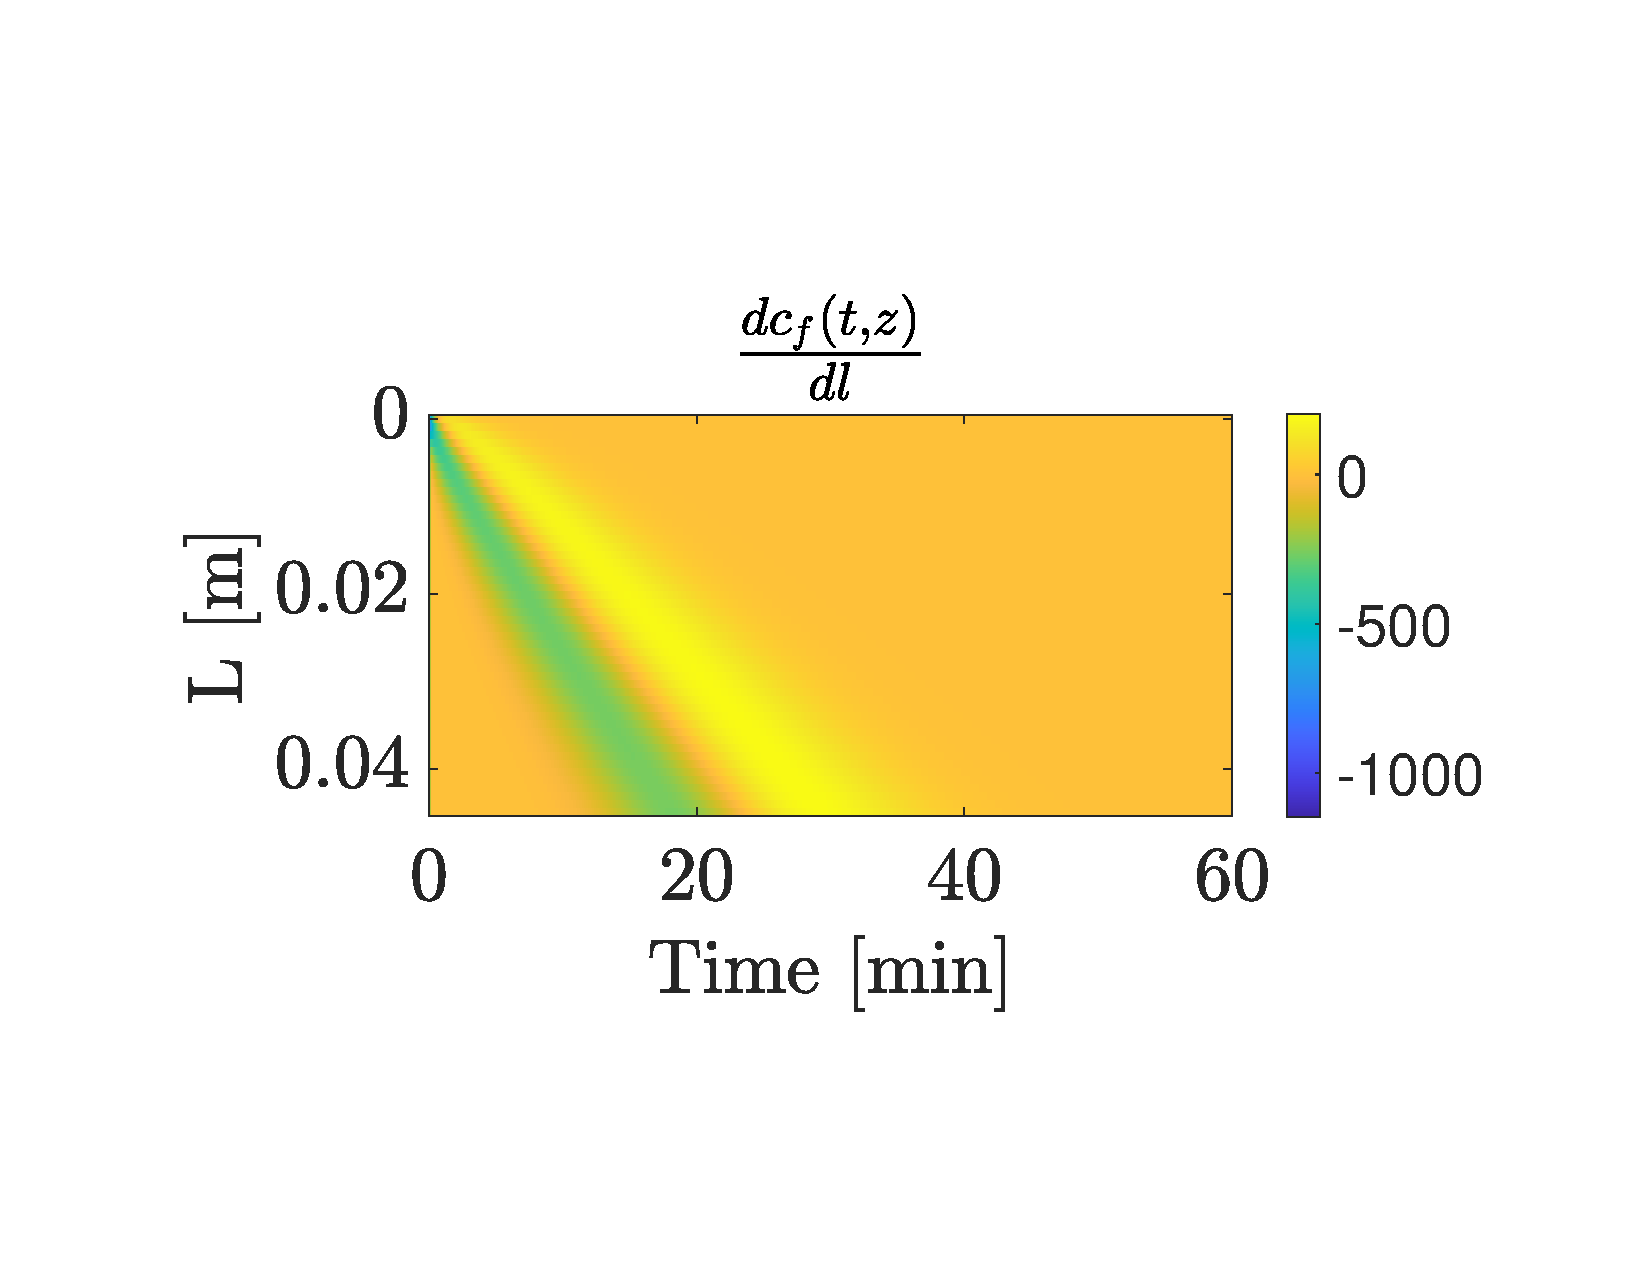
\includegraphics[trim = 3cm 4cm 2.5cm 4.3cm,clip,width=0.32\linewidth]{Figures/Sensitivity/Imagesc/2SS_Rdp.pdf} };
				\node[xshift=-6.7cm,rotate=90] at (Liq2) {${\color{magenta}l}{\color{white}(t)}$};
				\node[inner sep=2pt] (Solid) at (12,-7)
				{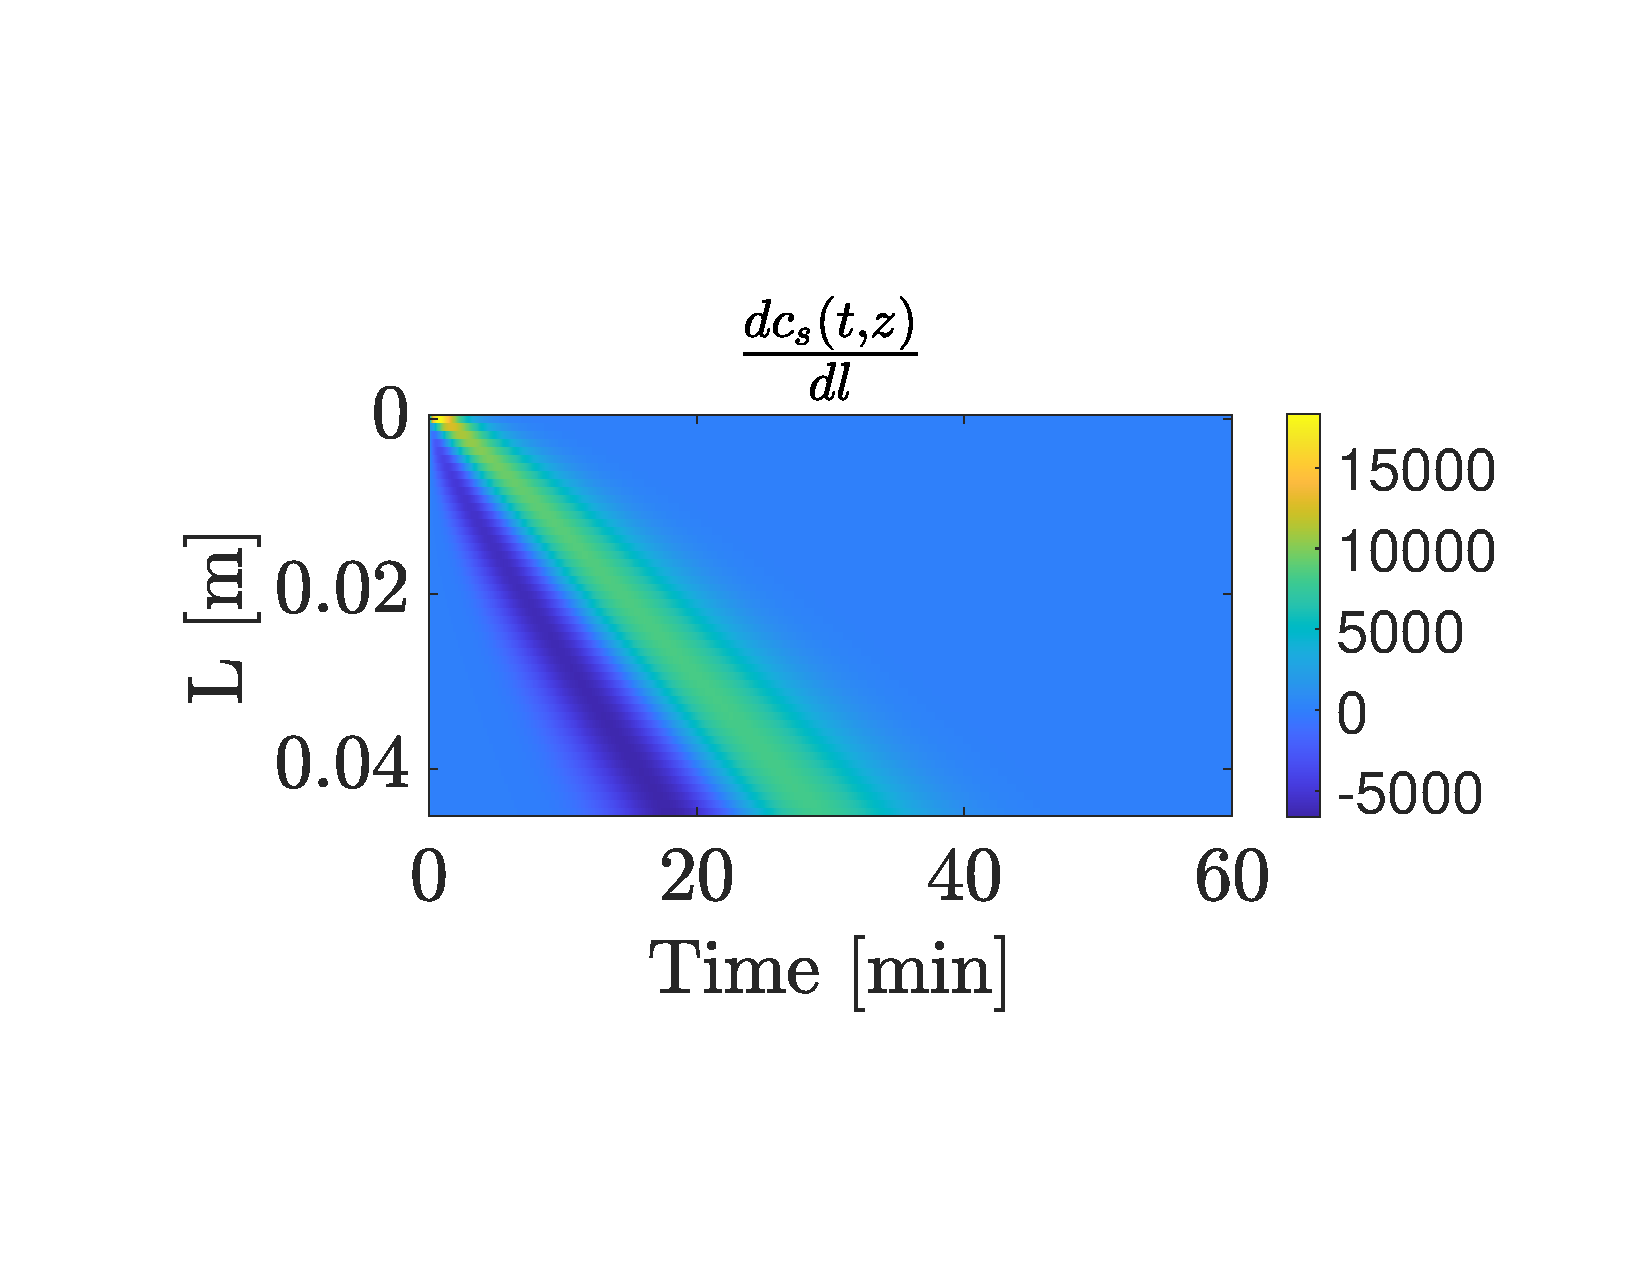
\includegraphics[trim = 3cm 4cm 2.5cm 4.3cm,clip,width=0.32\linewidth]{Figures/Sensitivity/Imagesc/3SS_Rdp.pdf} };
				\node[inner sep=2pt] (Yield) at (24,-7)
				{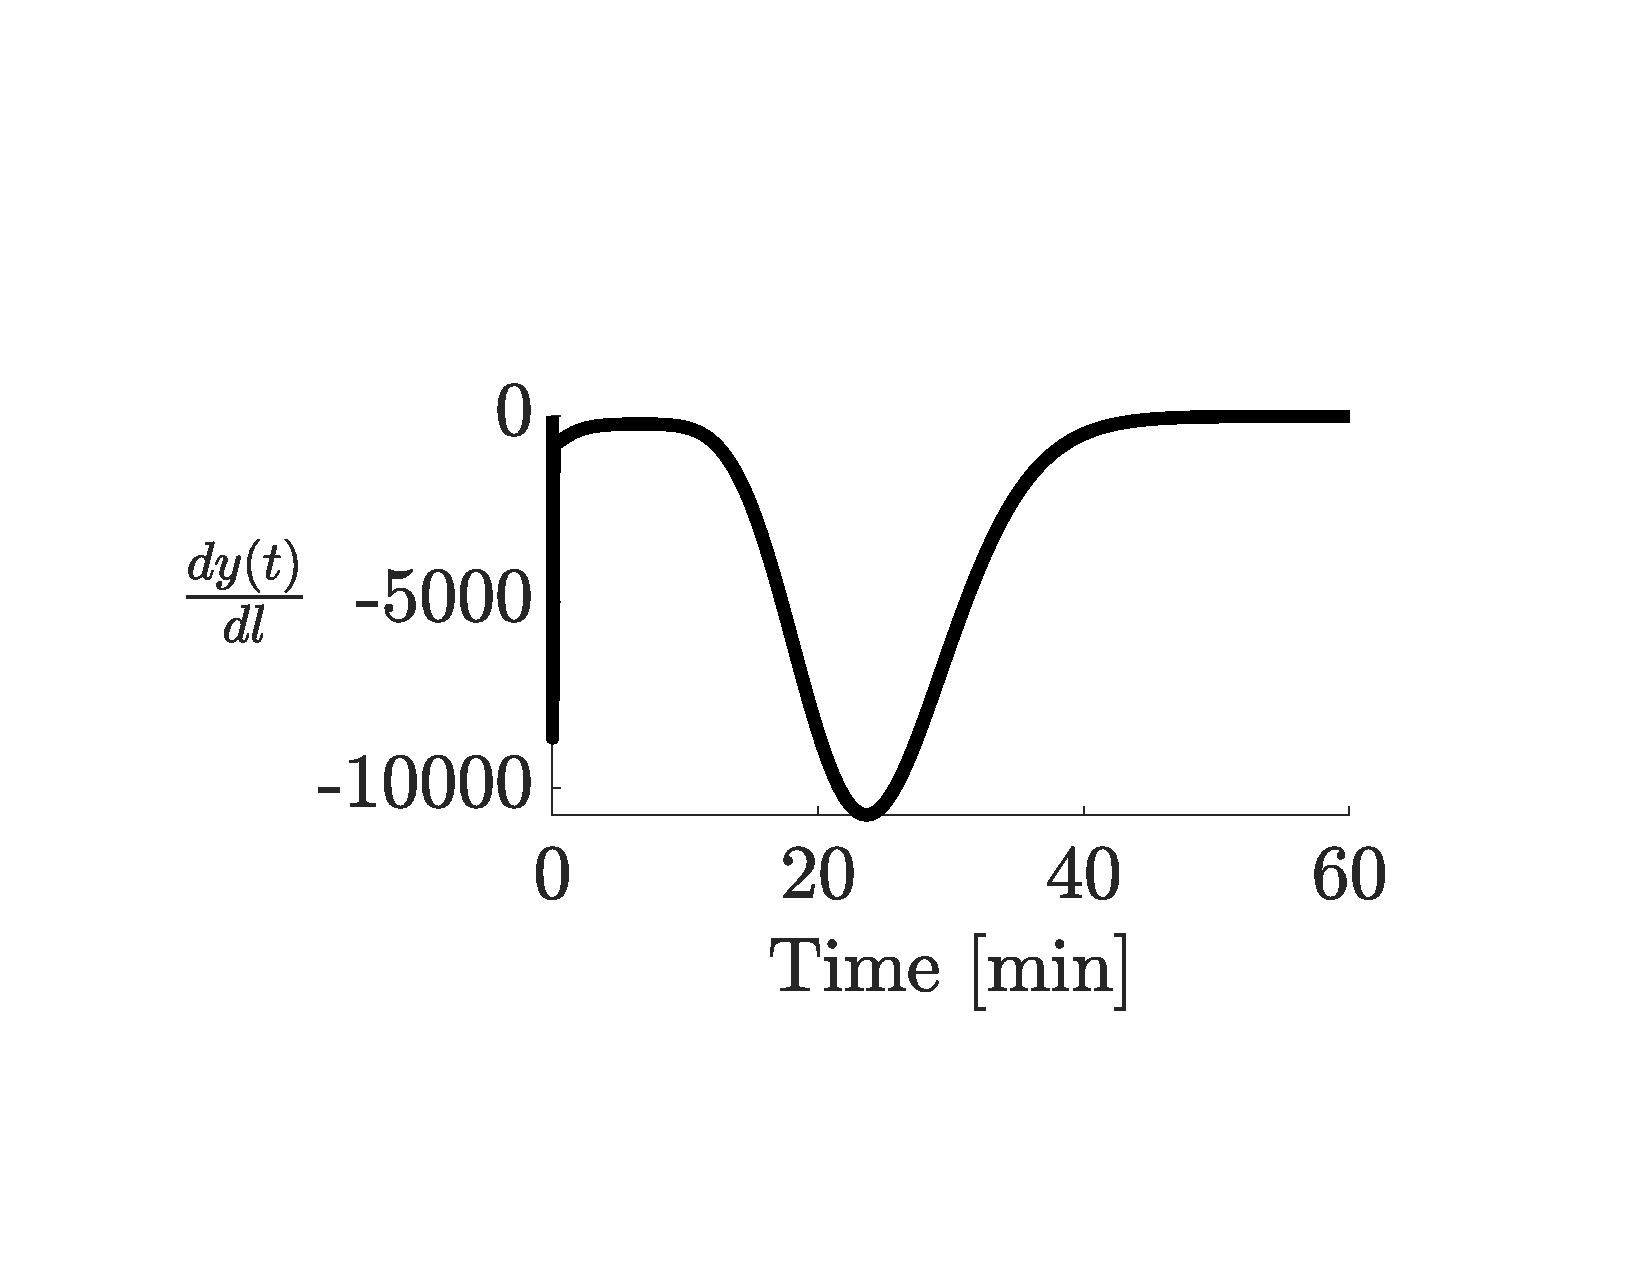
\includegraphics[trim = 3cm 4cm 2.5cm 4.3cm,clip,width=0.32\linewidth]{Figures/Sensitivity/Imagesc/1SS_Rdp.pdf} };
			\end{tikzpicture}
			\captionof{figure}{Results of the sensitivity analysis with respect to selected model parameters}  \label{Sensitivty_Parameters}

%			\begin{tikzfigure}
%				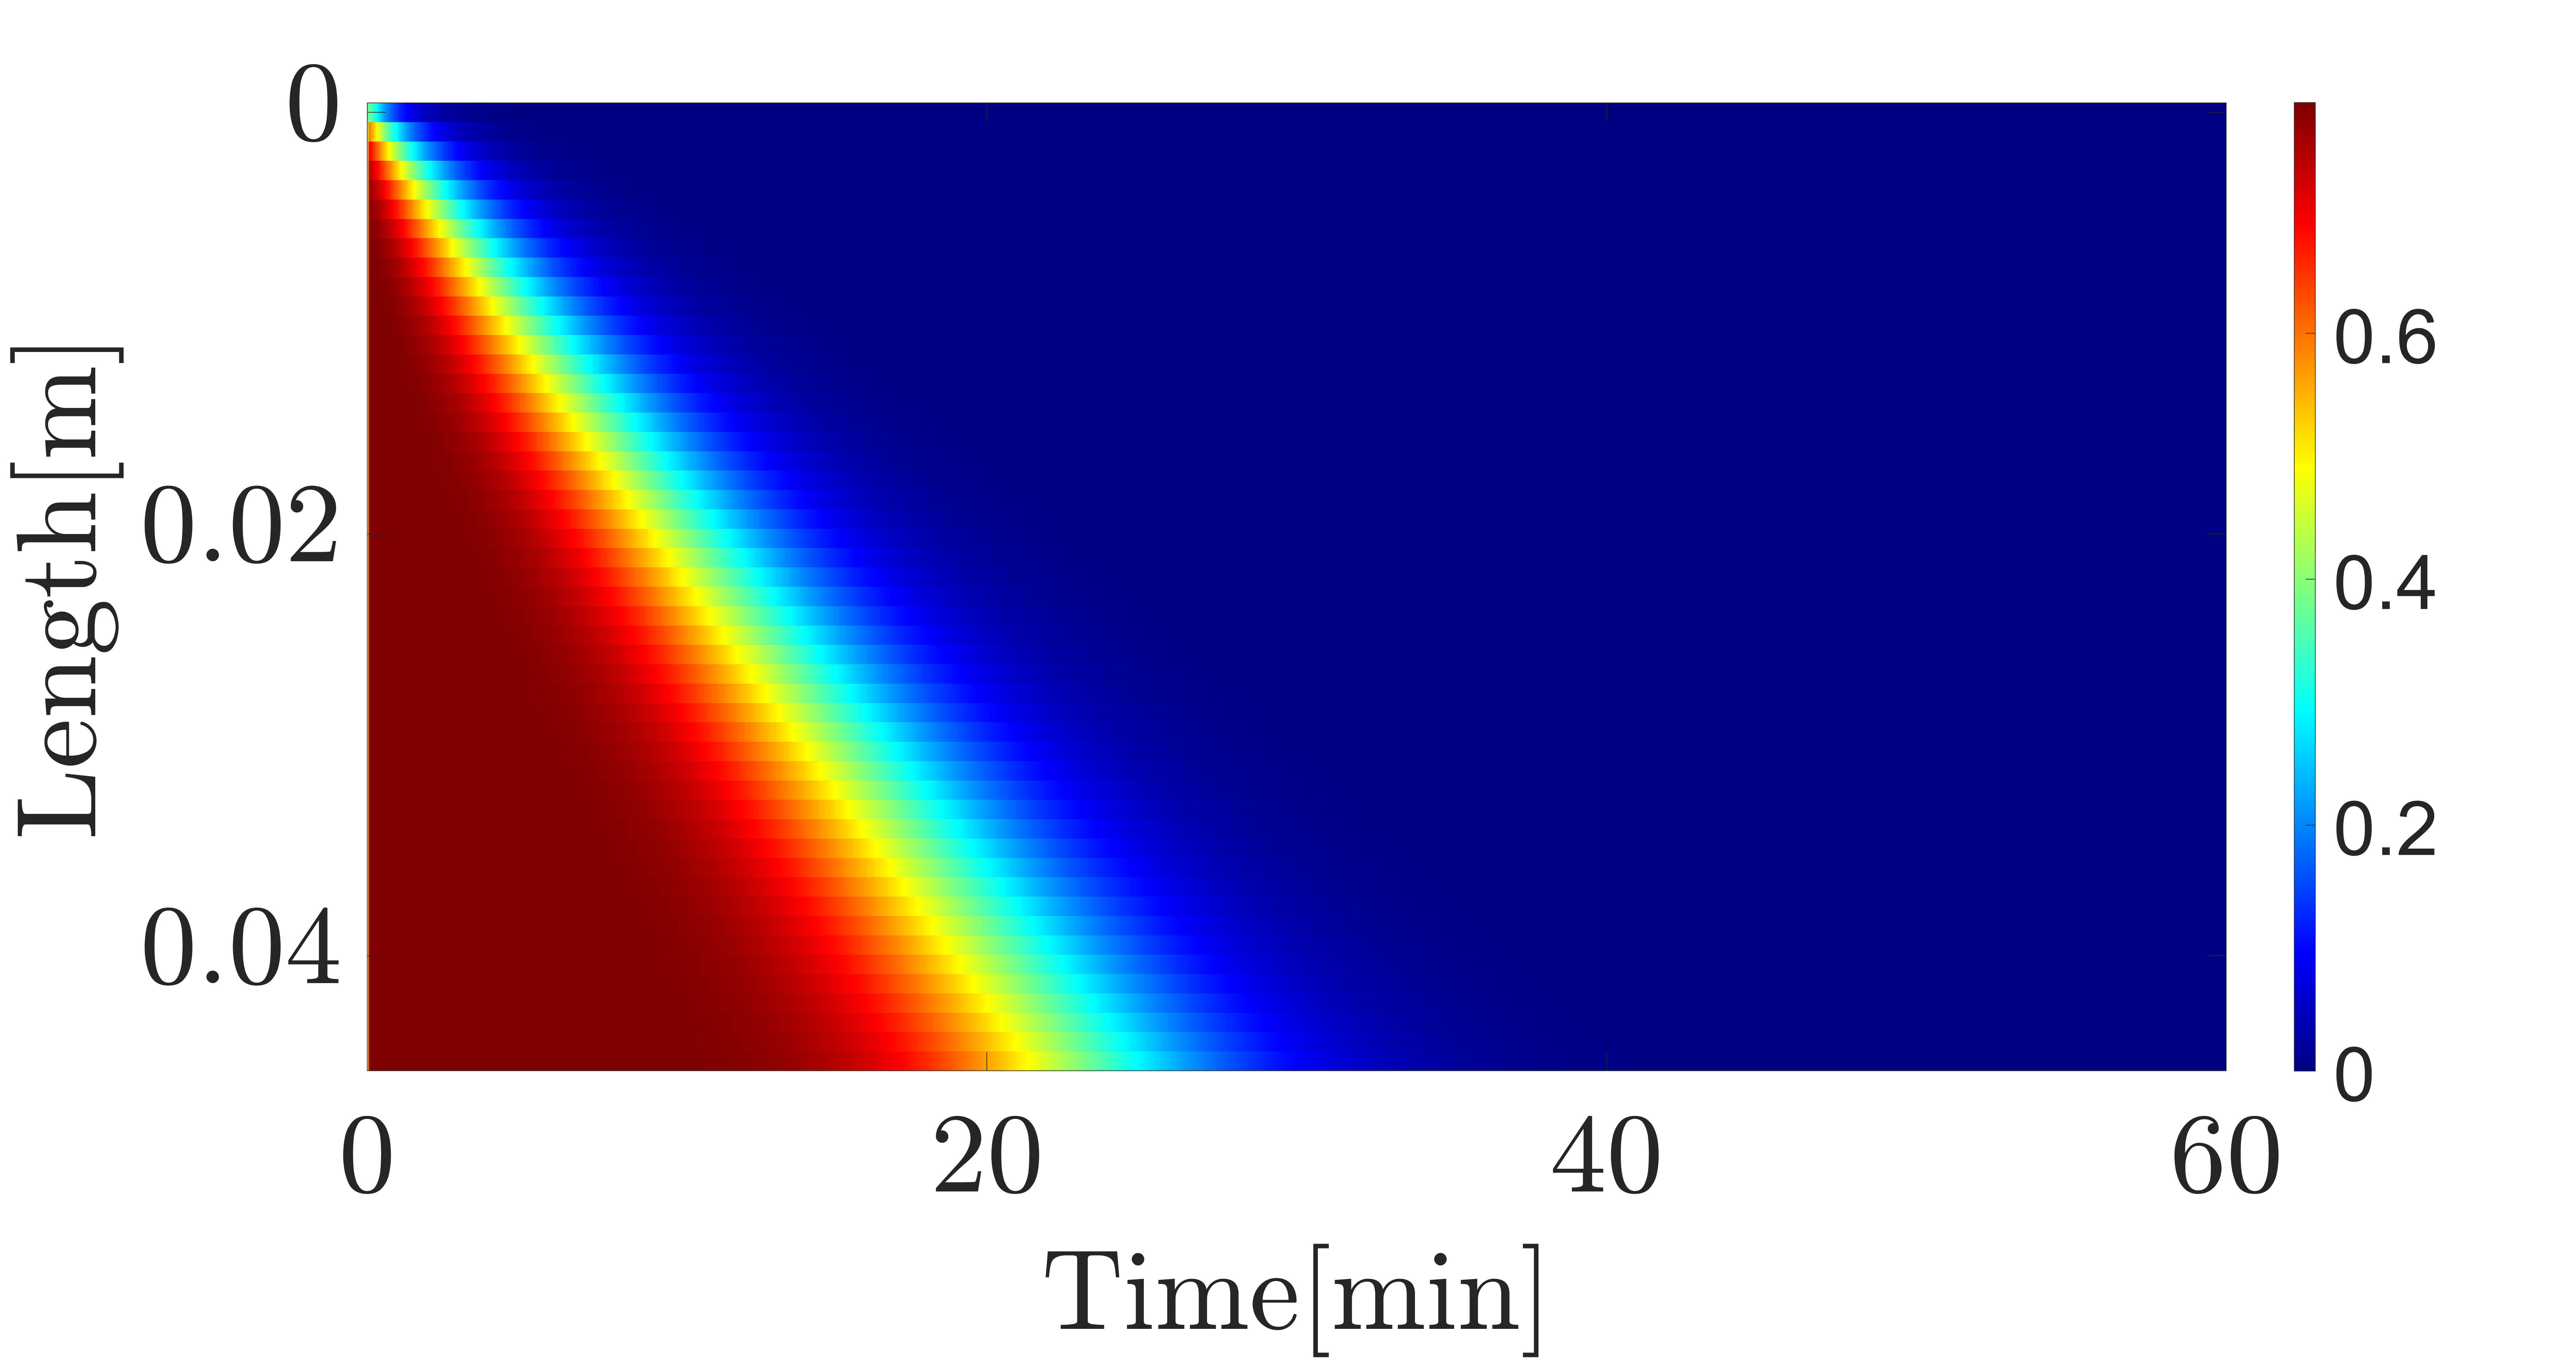
\includegraphics[width=0.32\linewidth]{Figures/Sensitivity/ConcentrationLiquid.png}         	
%				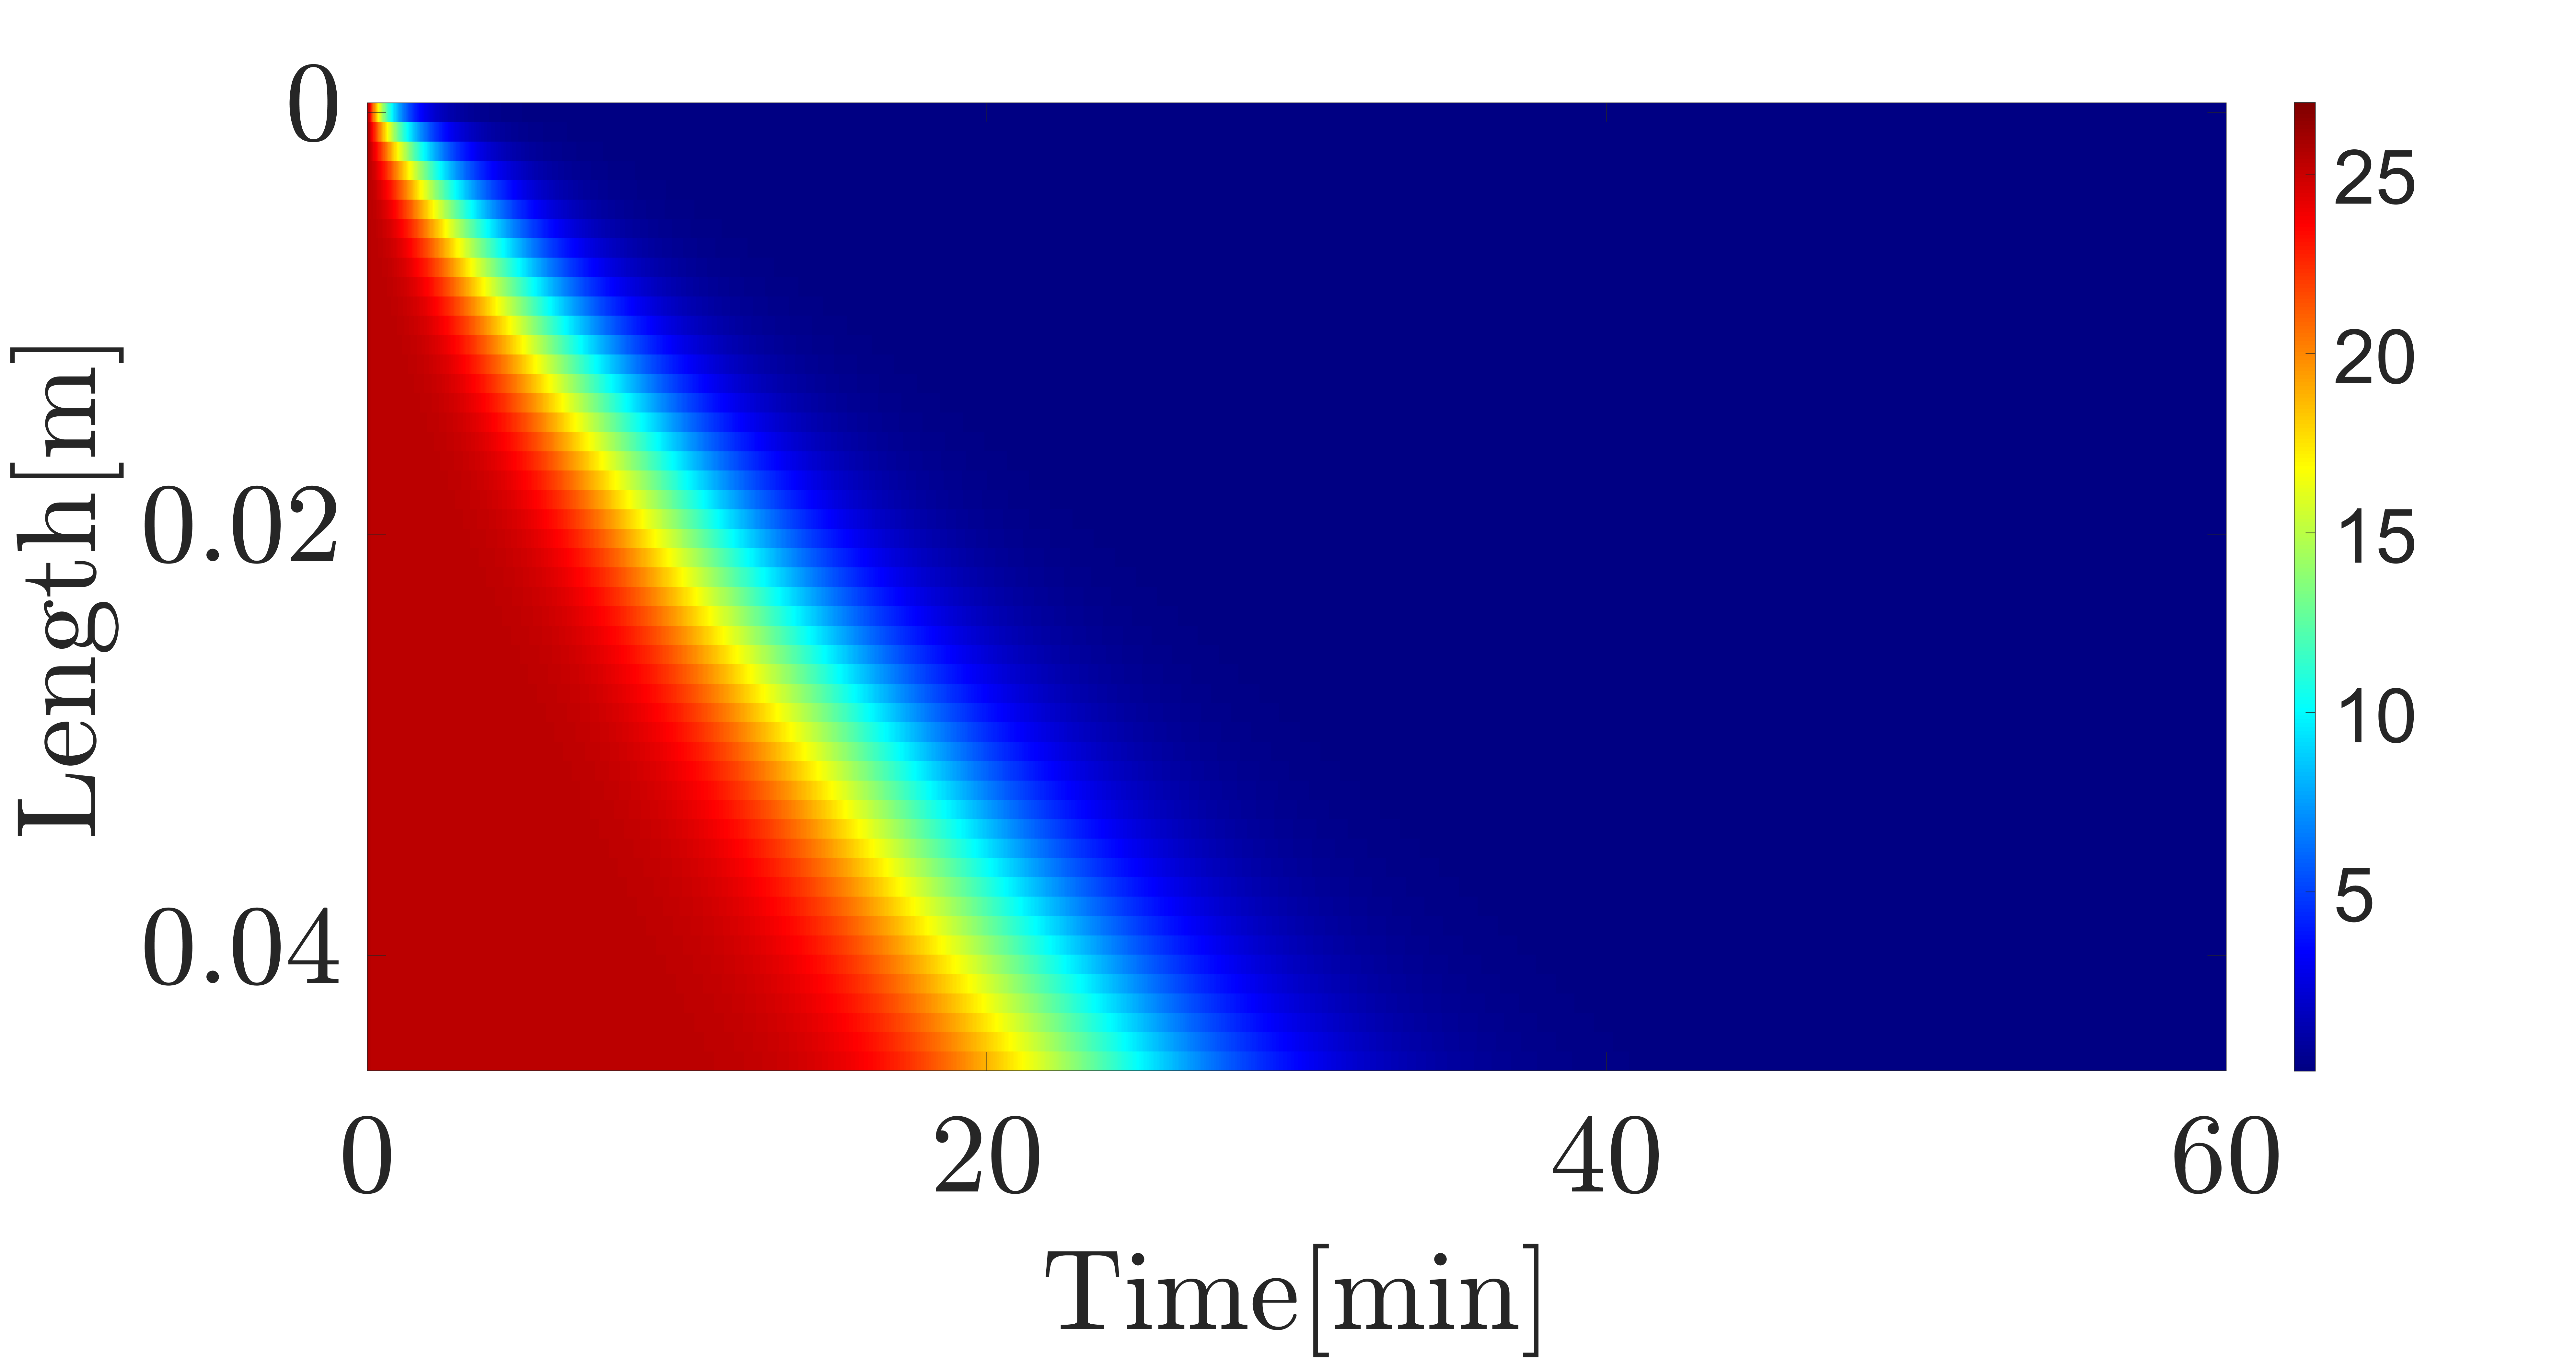
\includegraphics[width=0.32\linewidth]{Figures/Sensitivity/ConcentrationSolid.png}
%				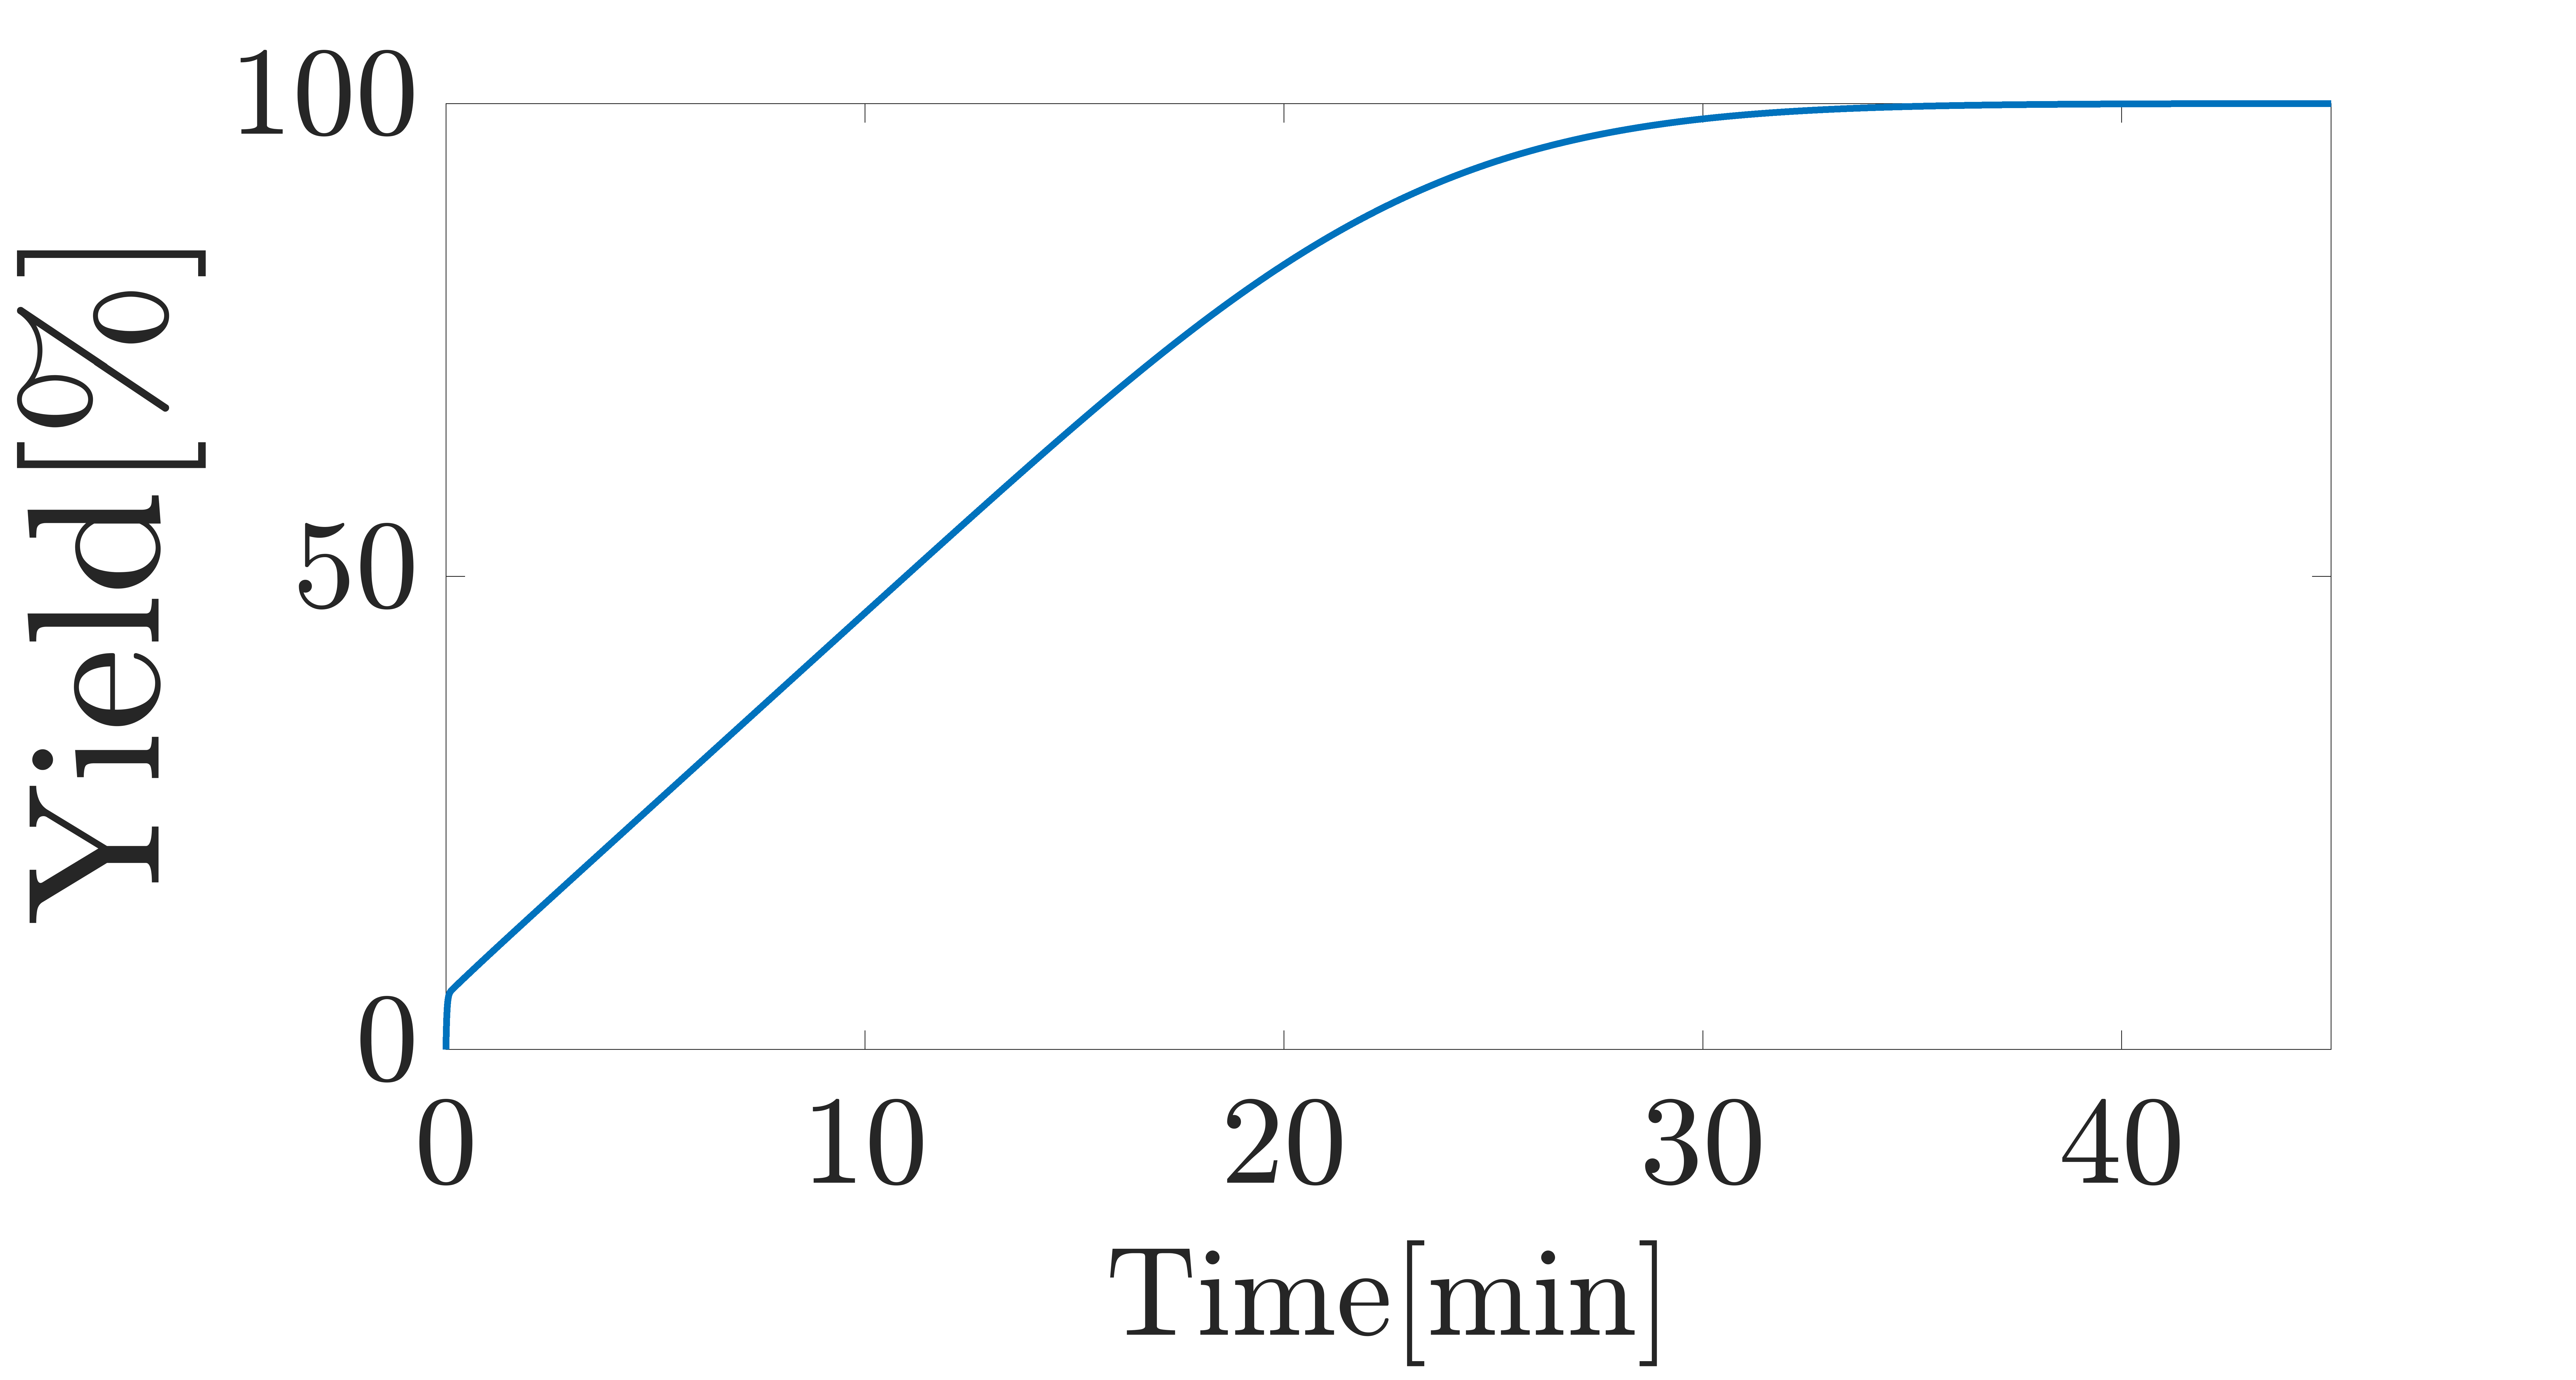
\includegraphics[width=0.32\linewidth]{Figures/Sensitivity/Yield.png}
%			\end{tikzfigure}
%			\captionof{figure}{Solution of the process model}
%			\hrule
%			\begin{tikzfigure}
%				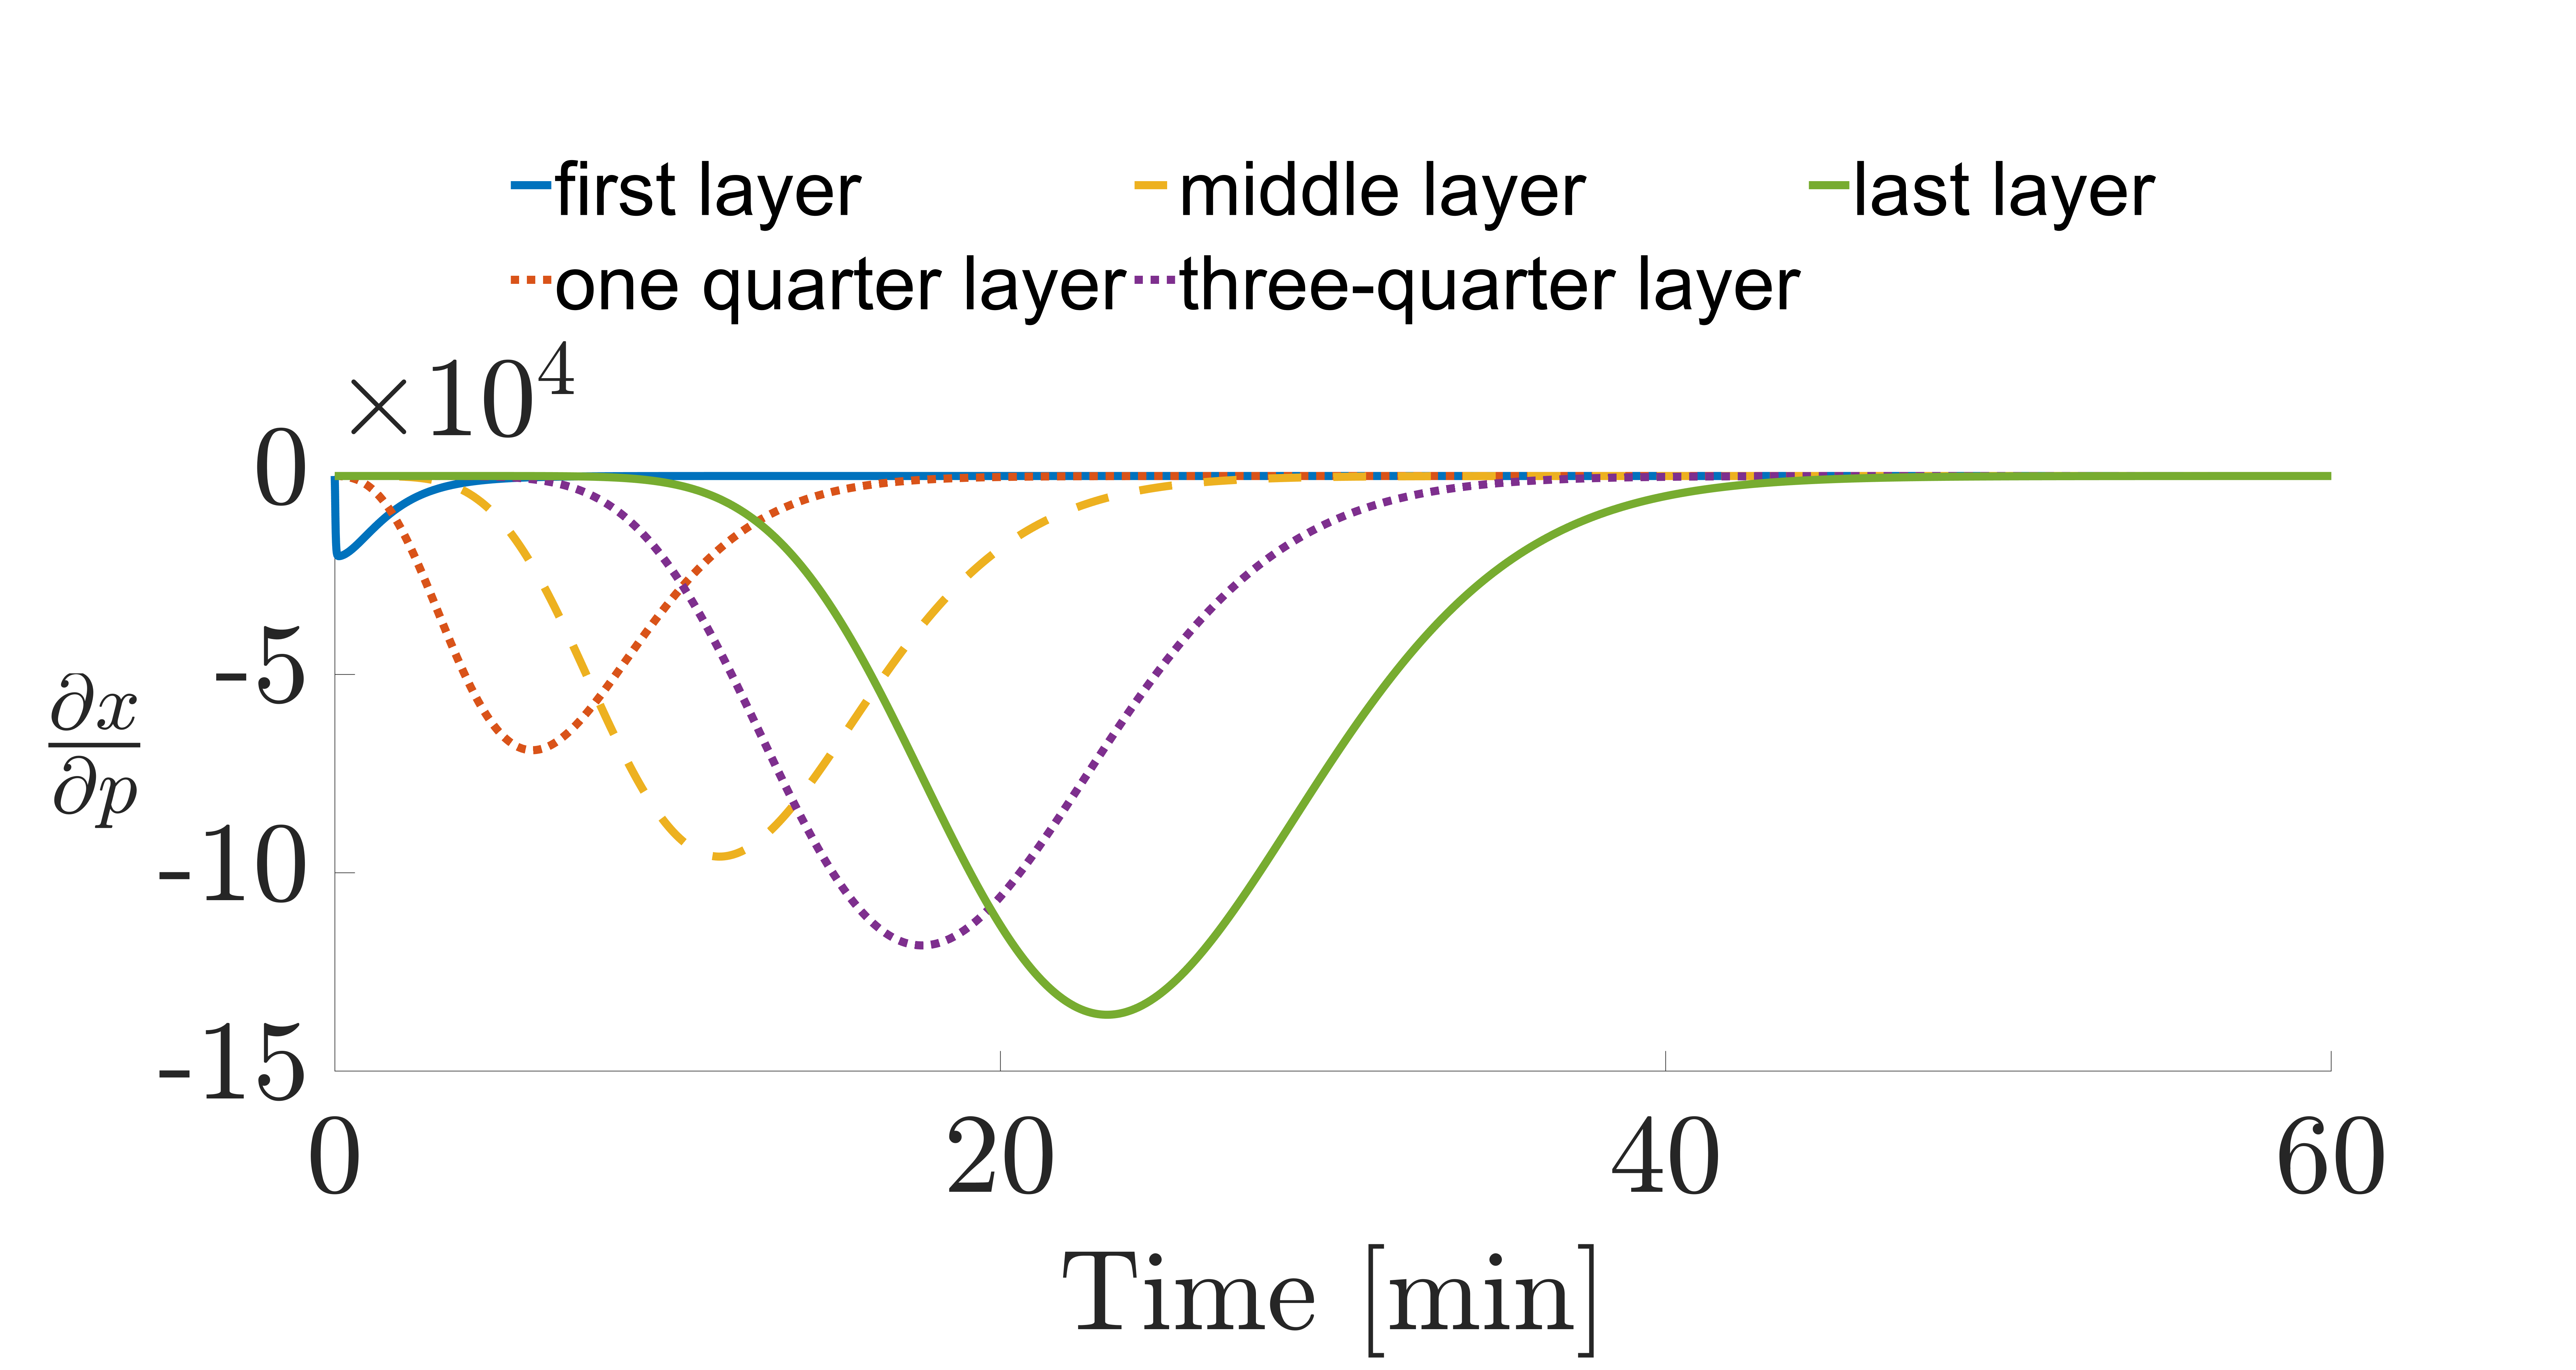
\includegraphics[width=0.32\linewidth]{Figures/Sensitivity/Imagesc/2_SS_R_F.png}
%				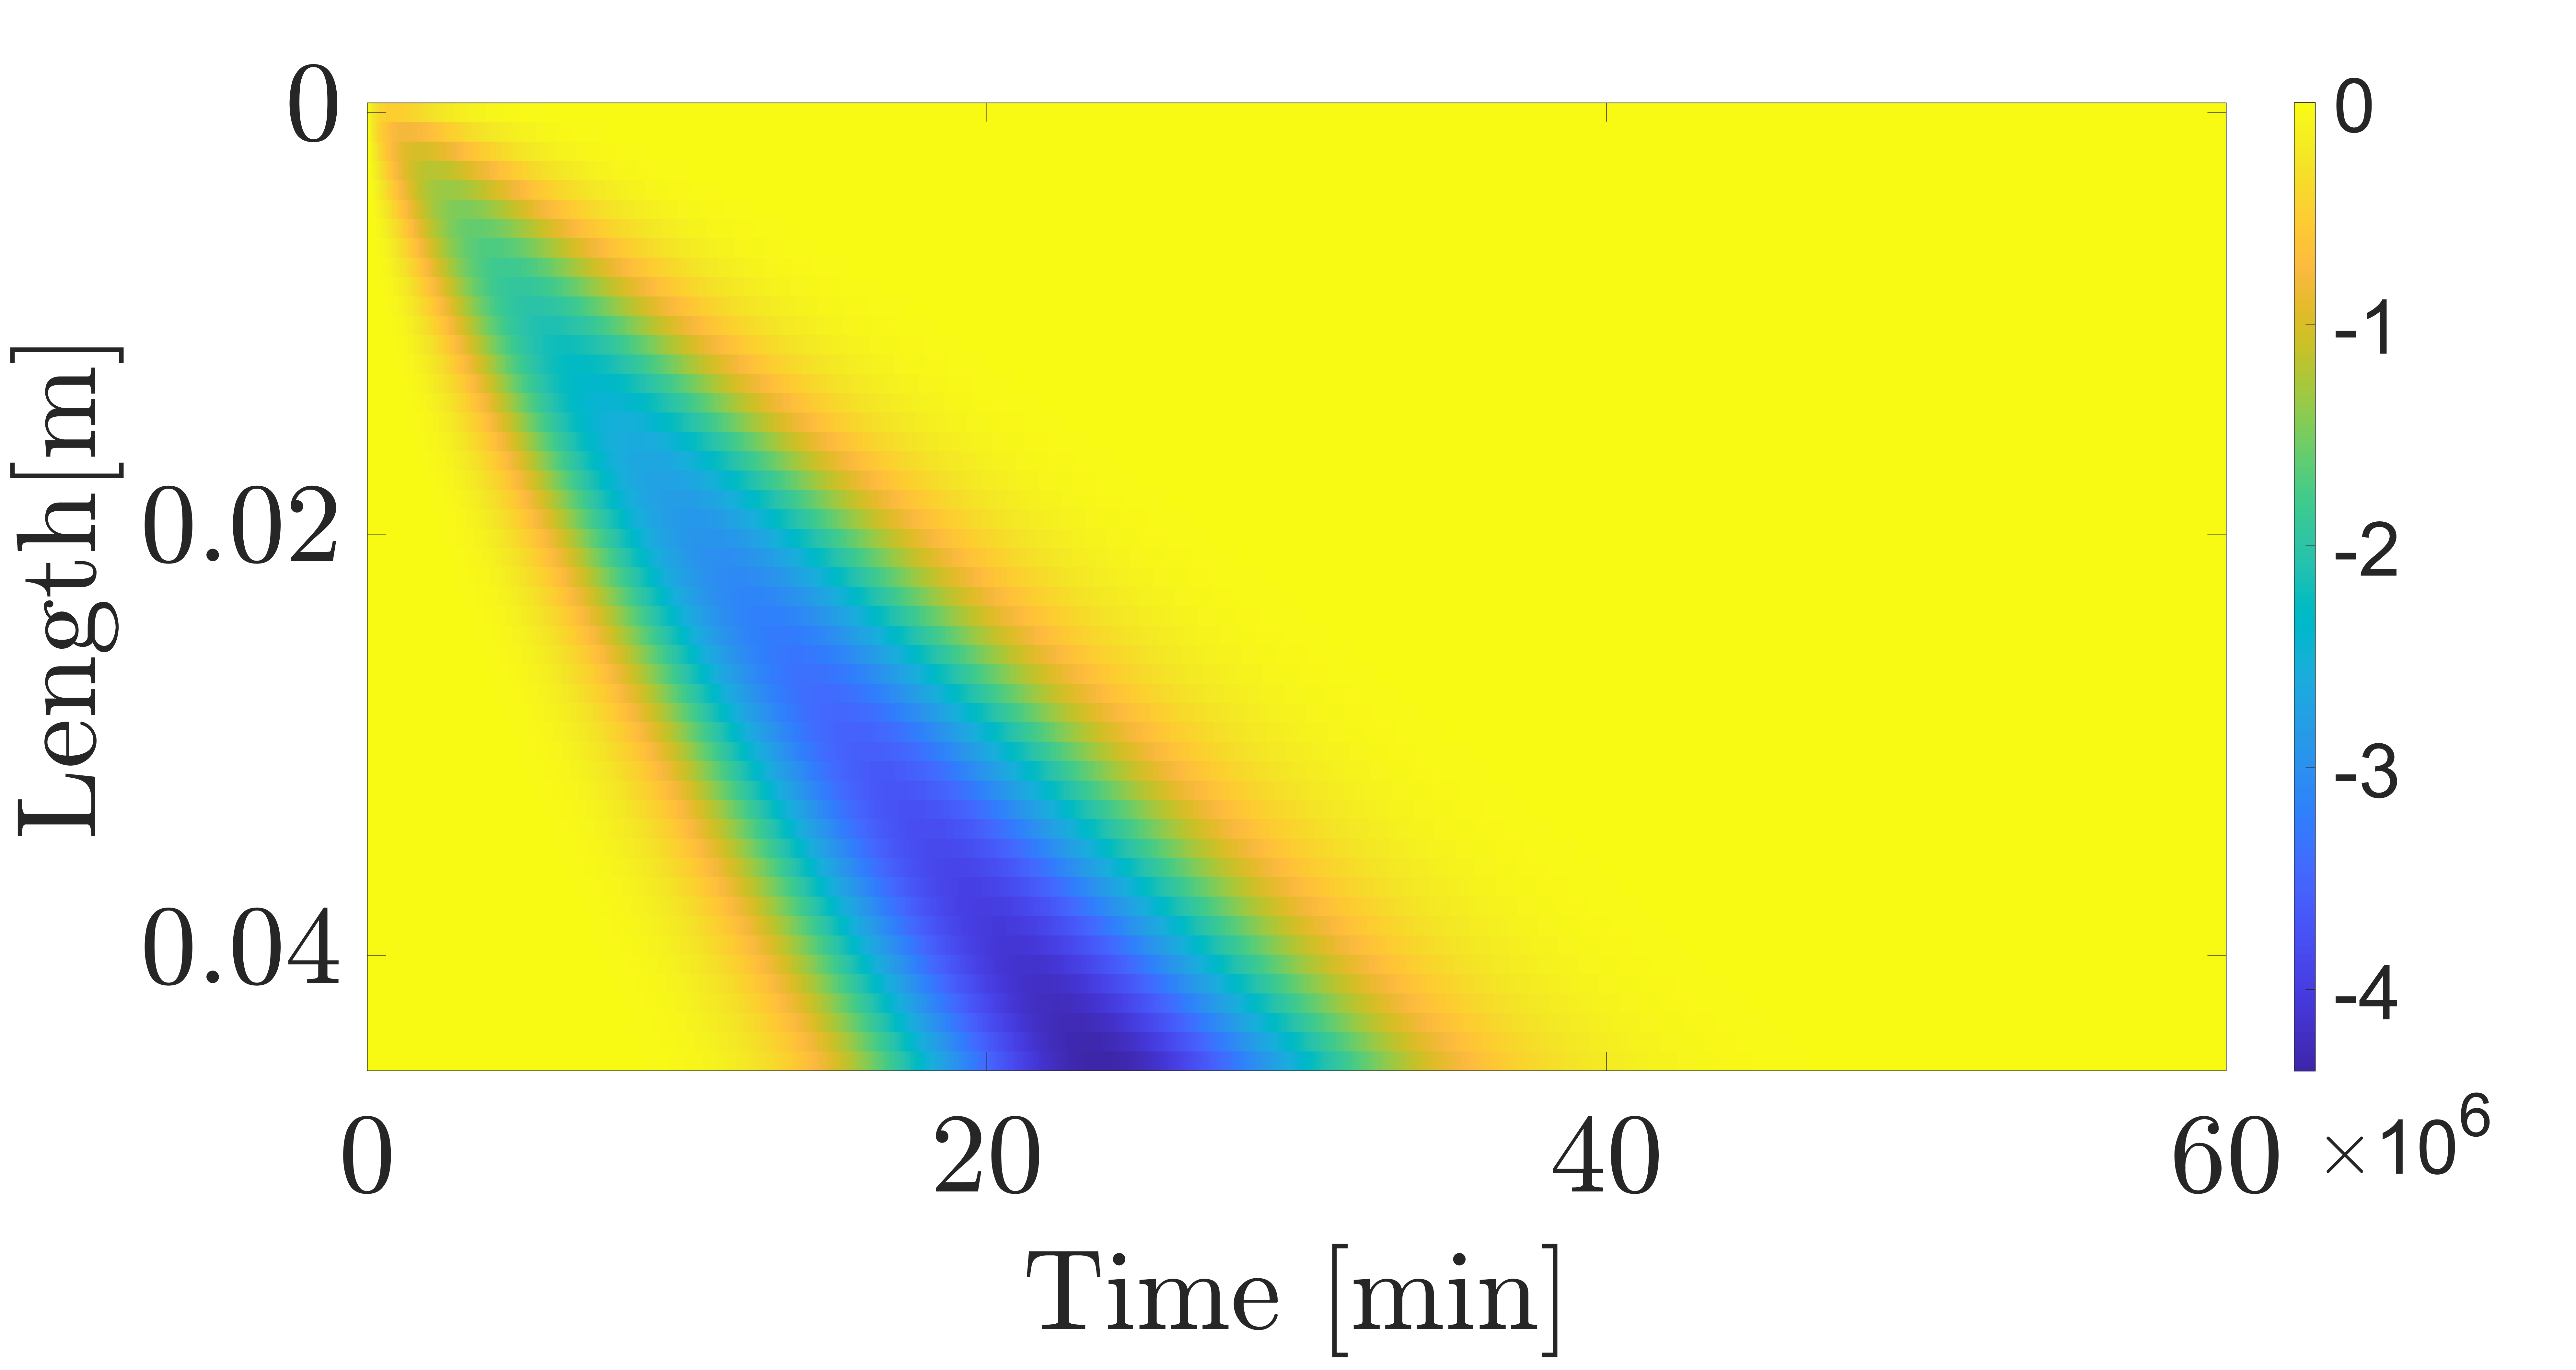
\includegraphics[width=0.32\linewidth]{Figures/Sensitivity/Imagesc/3_SS_R_F.png}
%				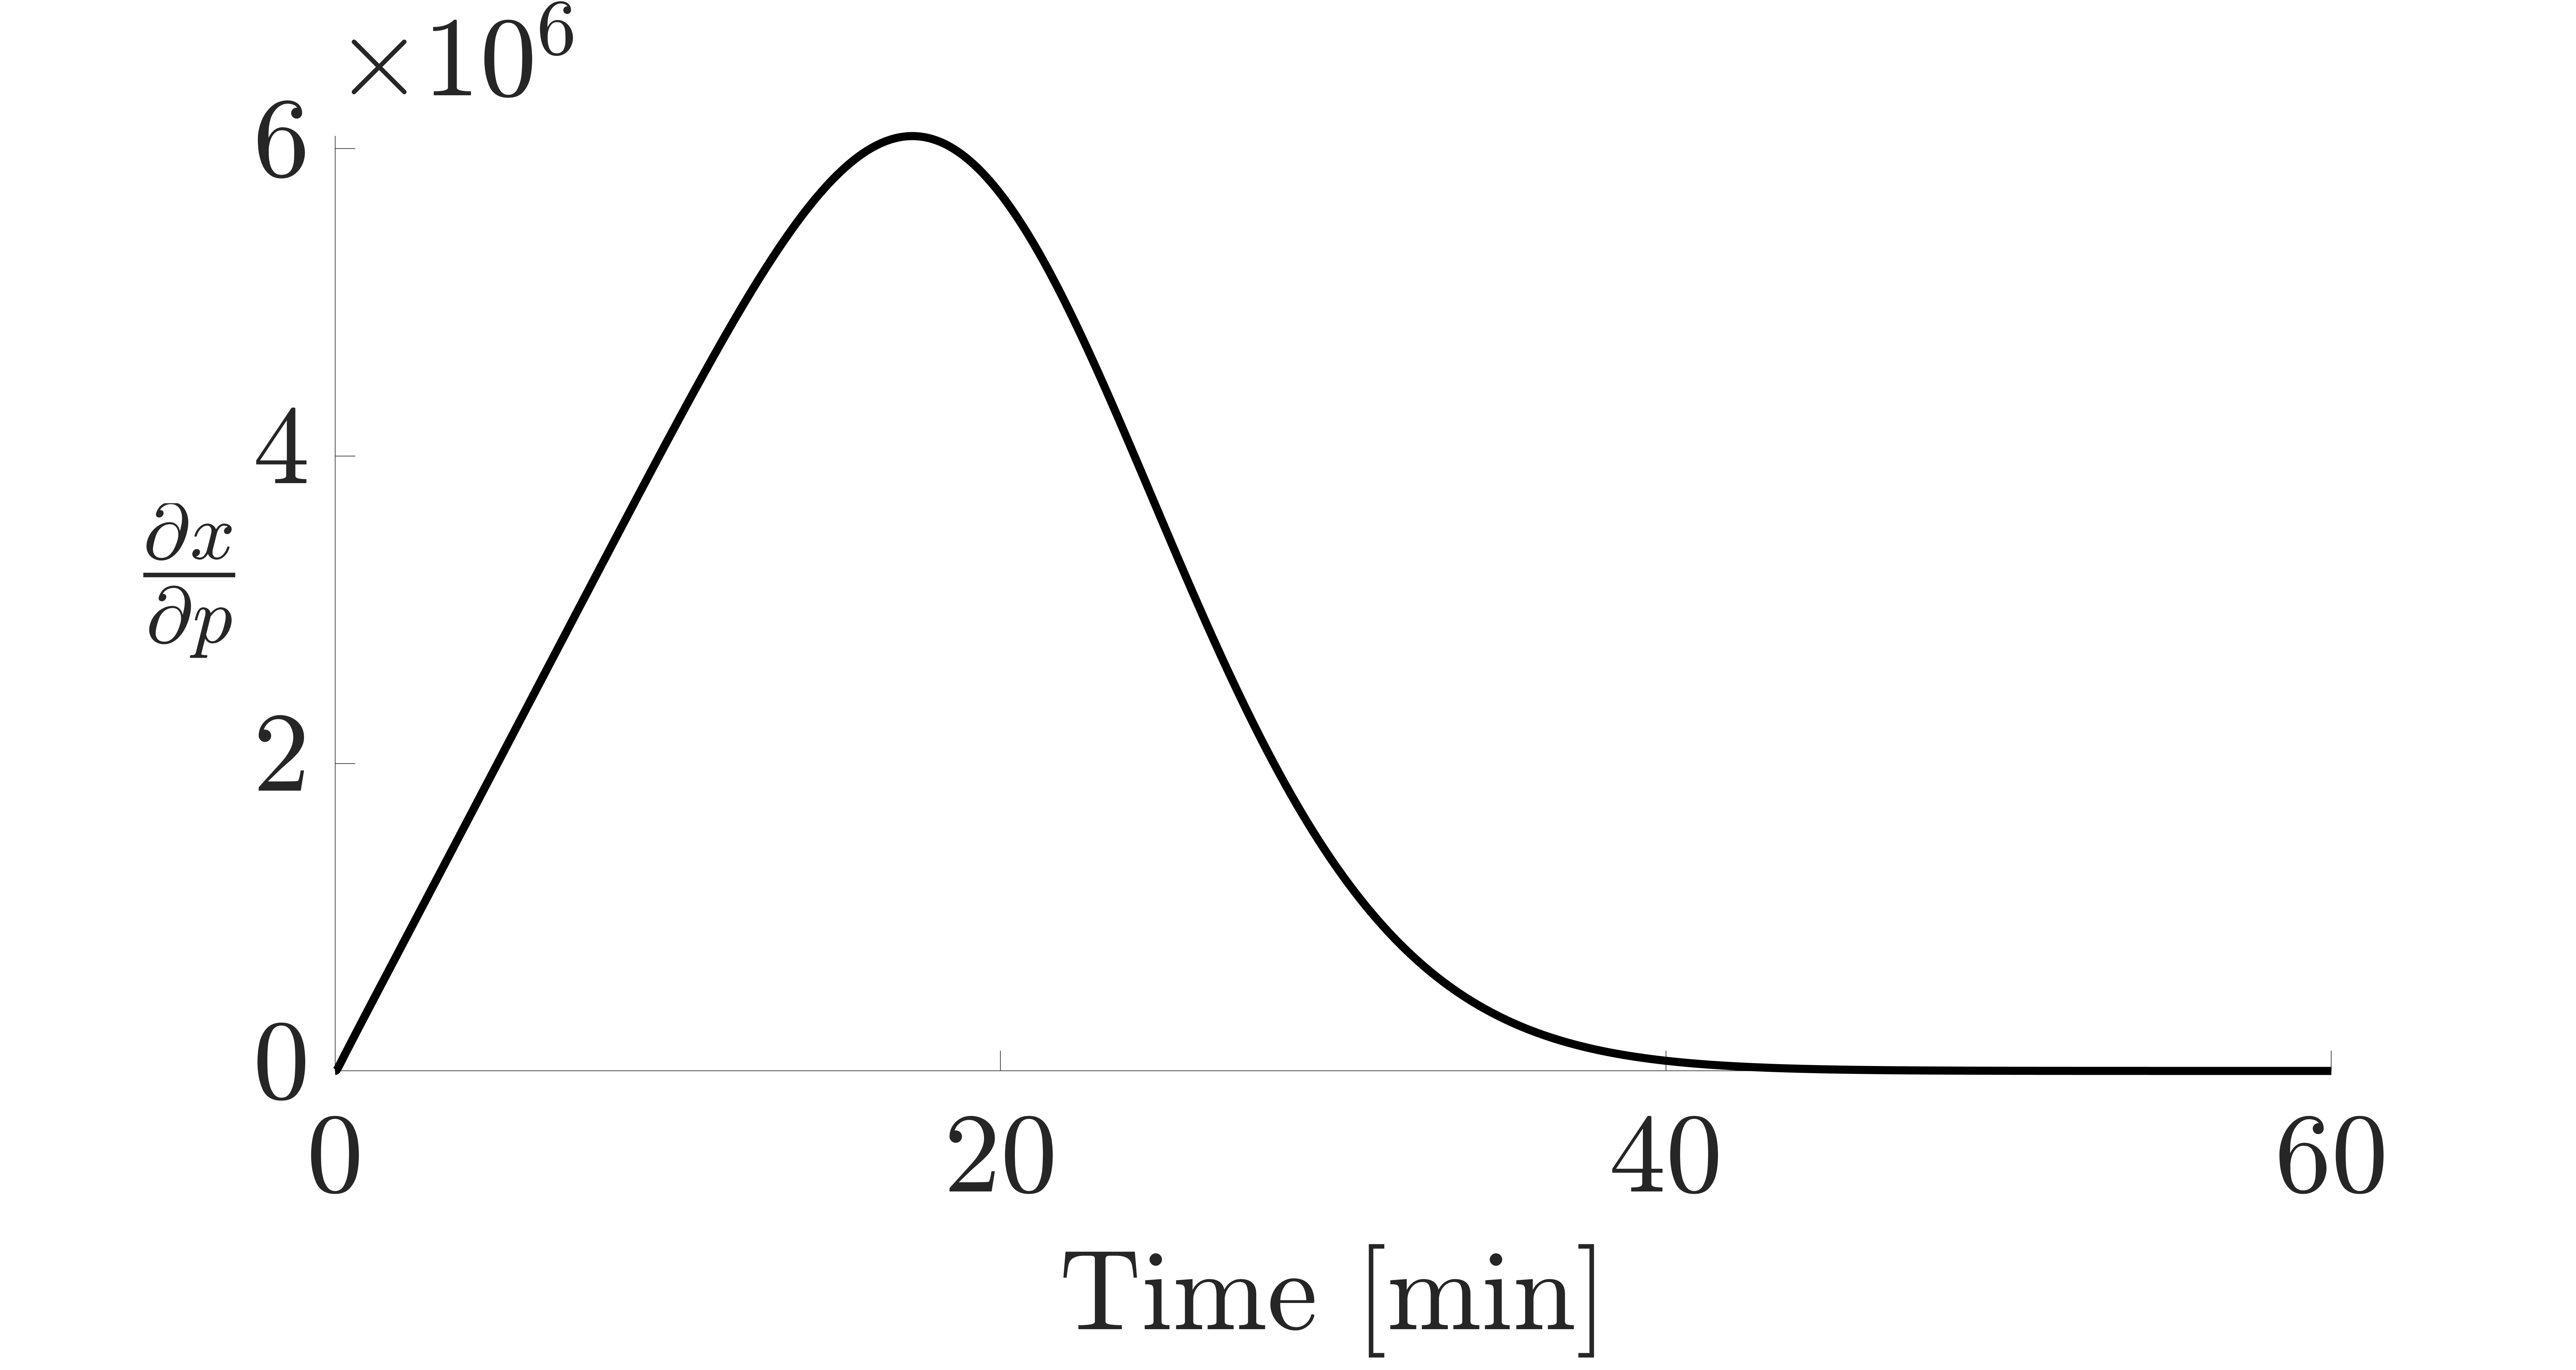
\includegraphics[width=0.32\linewidth]{Figures/Sensitivity/Plots/1_SS_R_F.png}
%			\end{tikzfigure}     
%			\captionof{figure}{Sensitivity with respect to the flowrate}
%			\begin{tikzfigure}
%				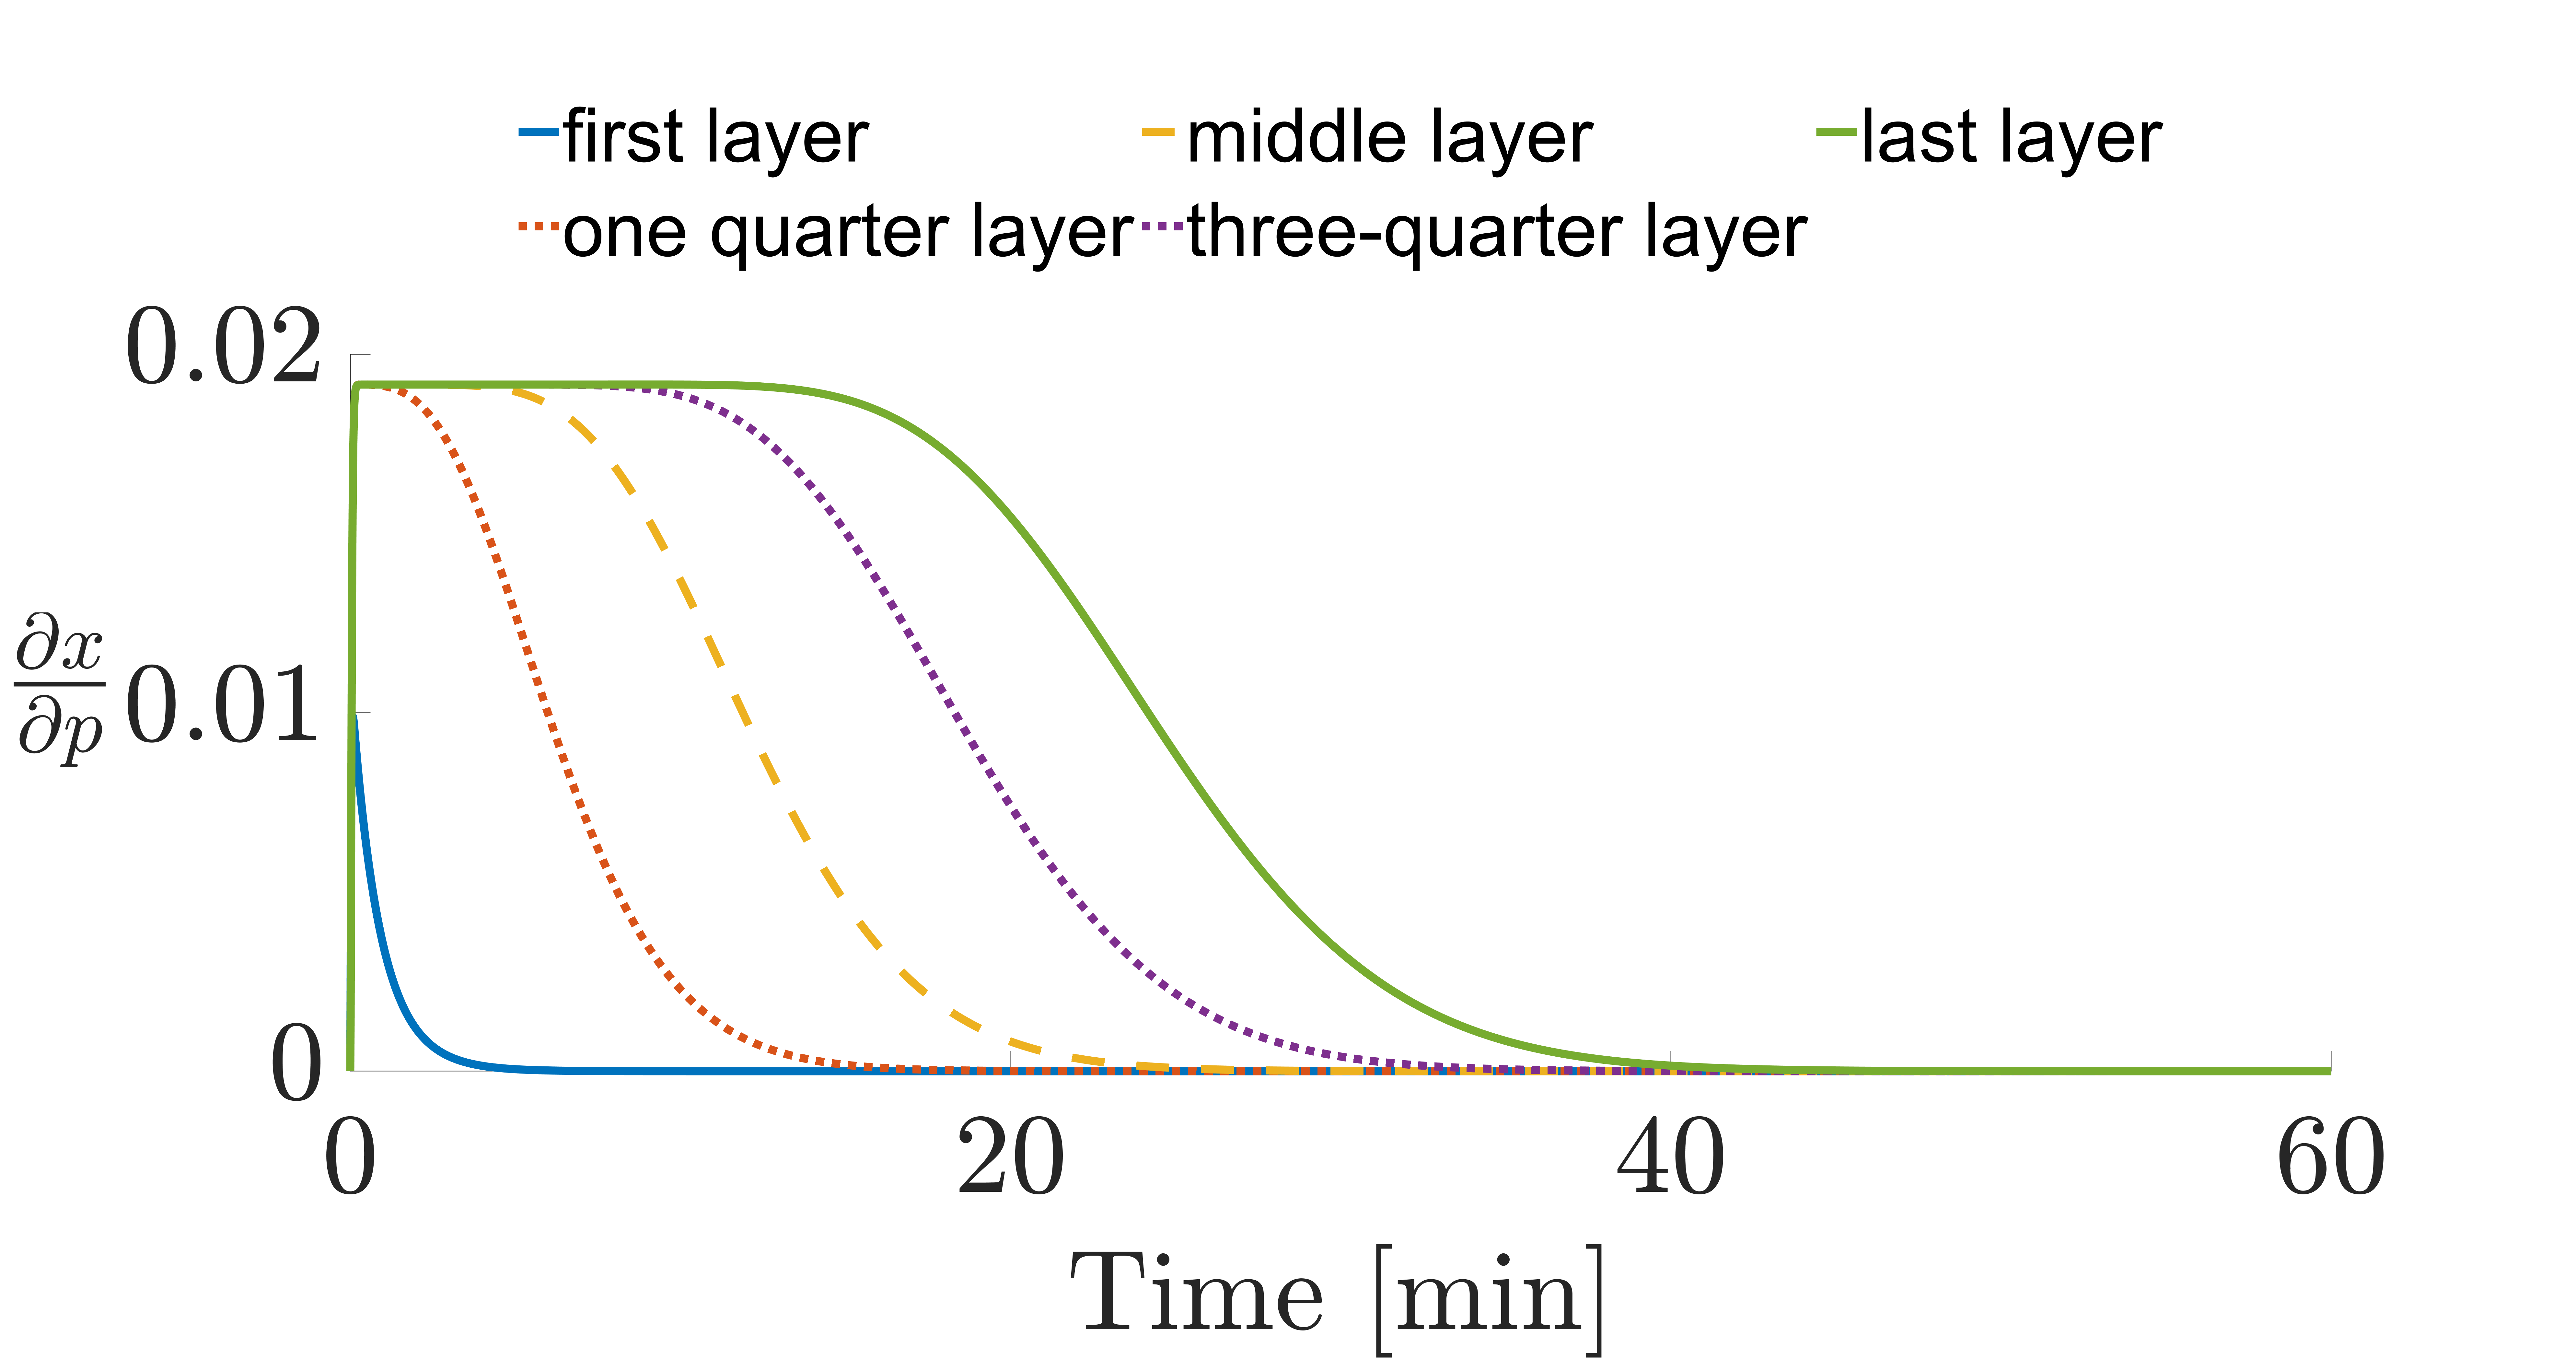
\includegraphics[width=0.32\linewidth]{Figures/Sensitivity/Imagesc/2_SS_R_P.png}
%				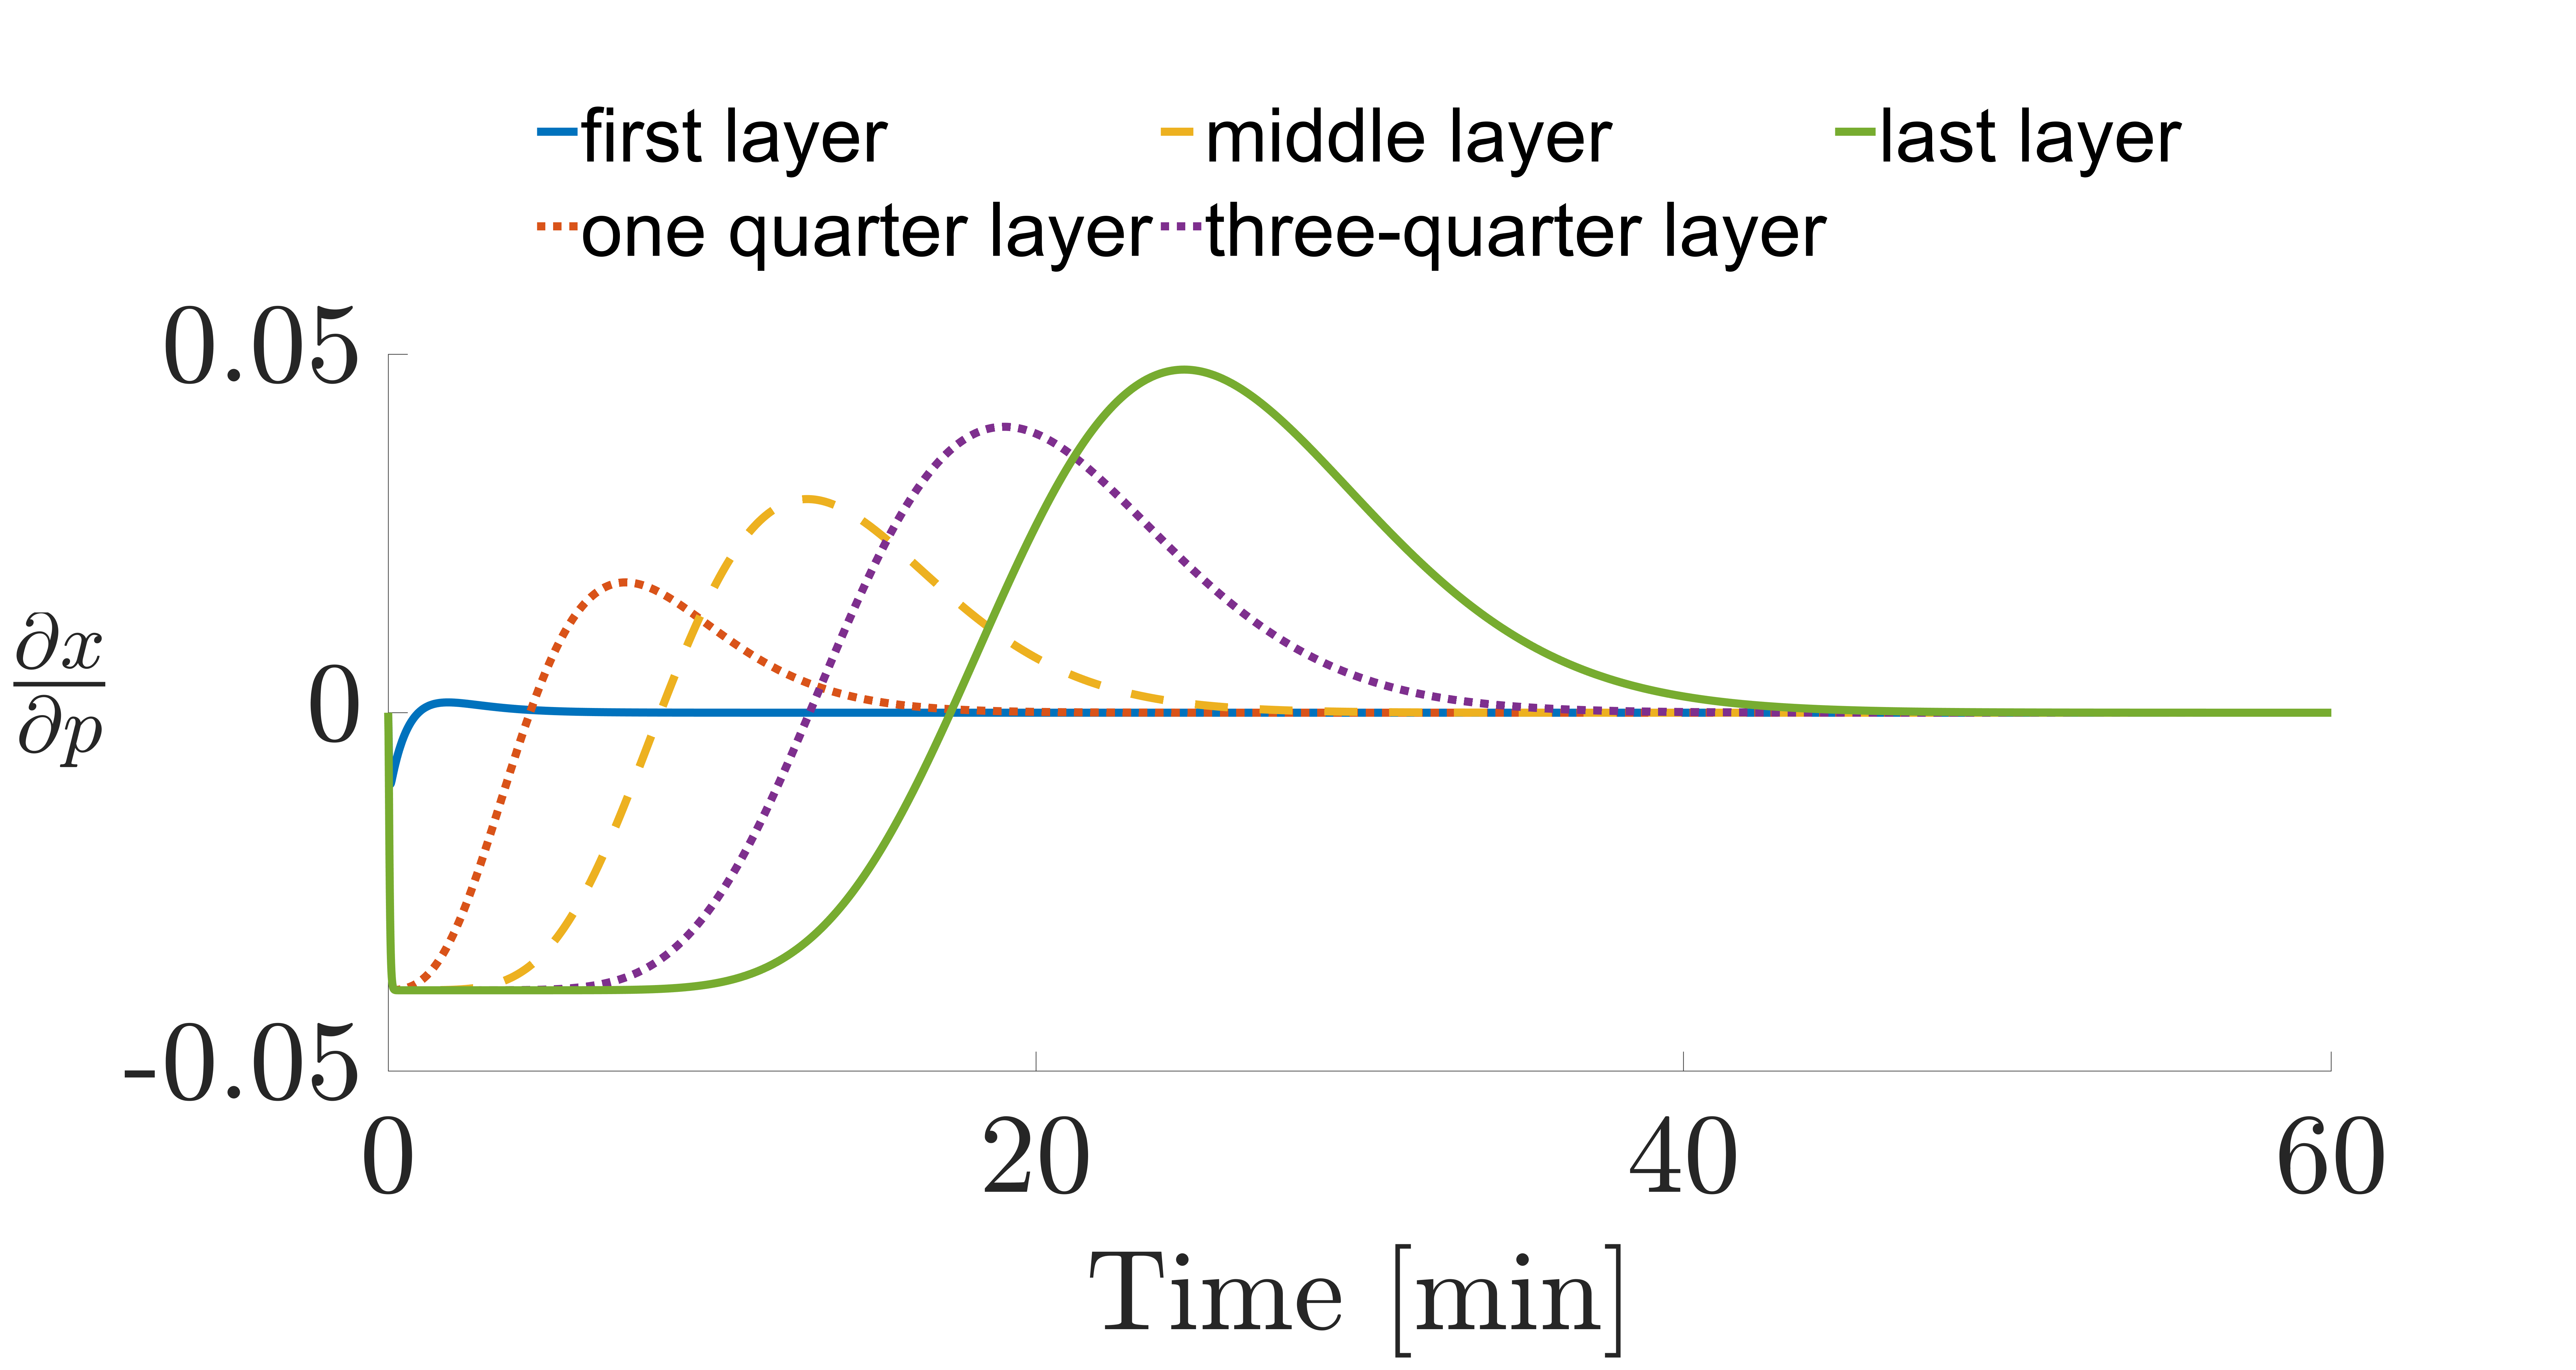
\includegraphics[width=0.32\linewidth]{Figures/Sensitivity/Imagesc/3_SS_R_P.png}
%				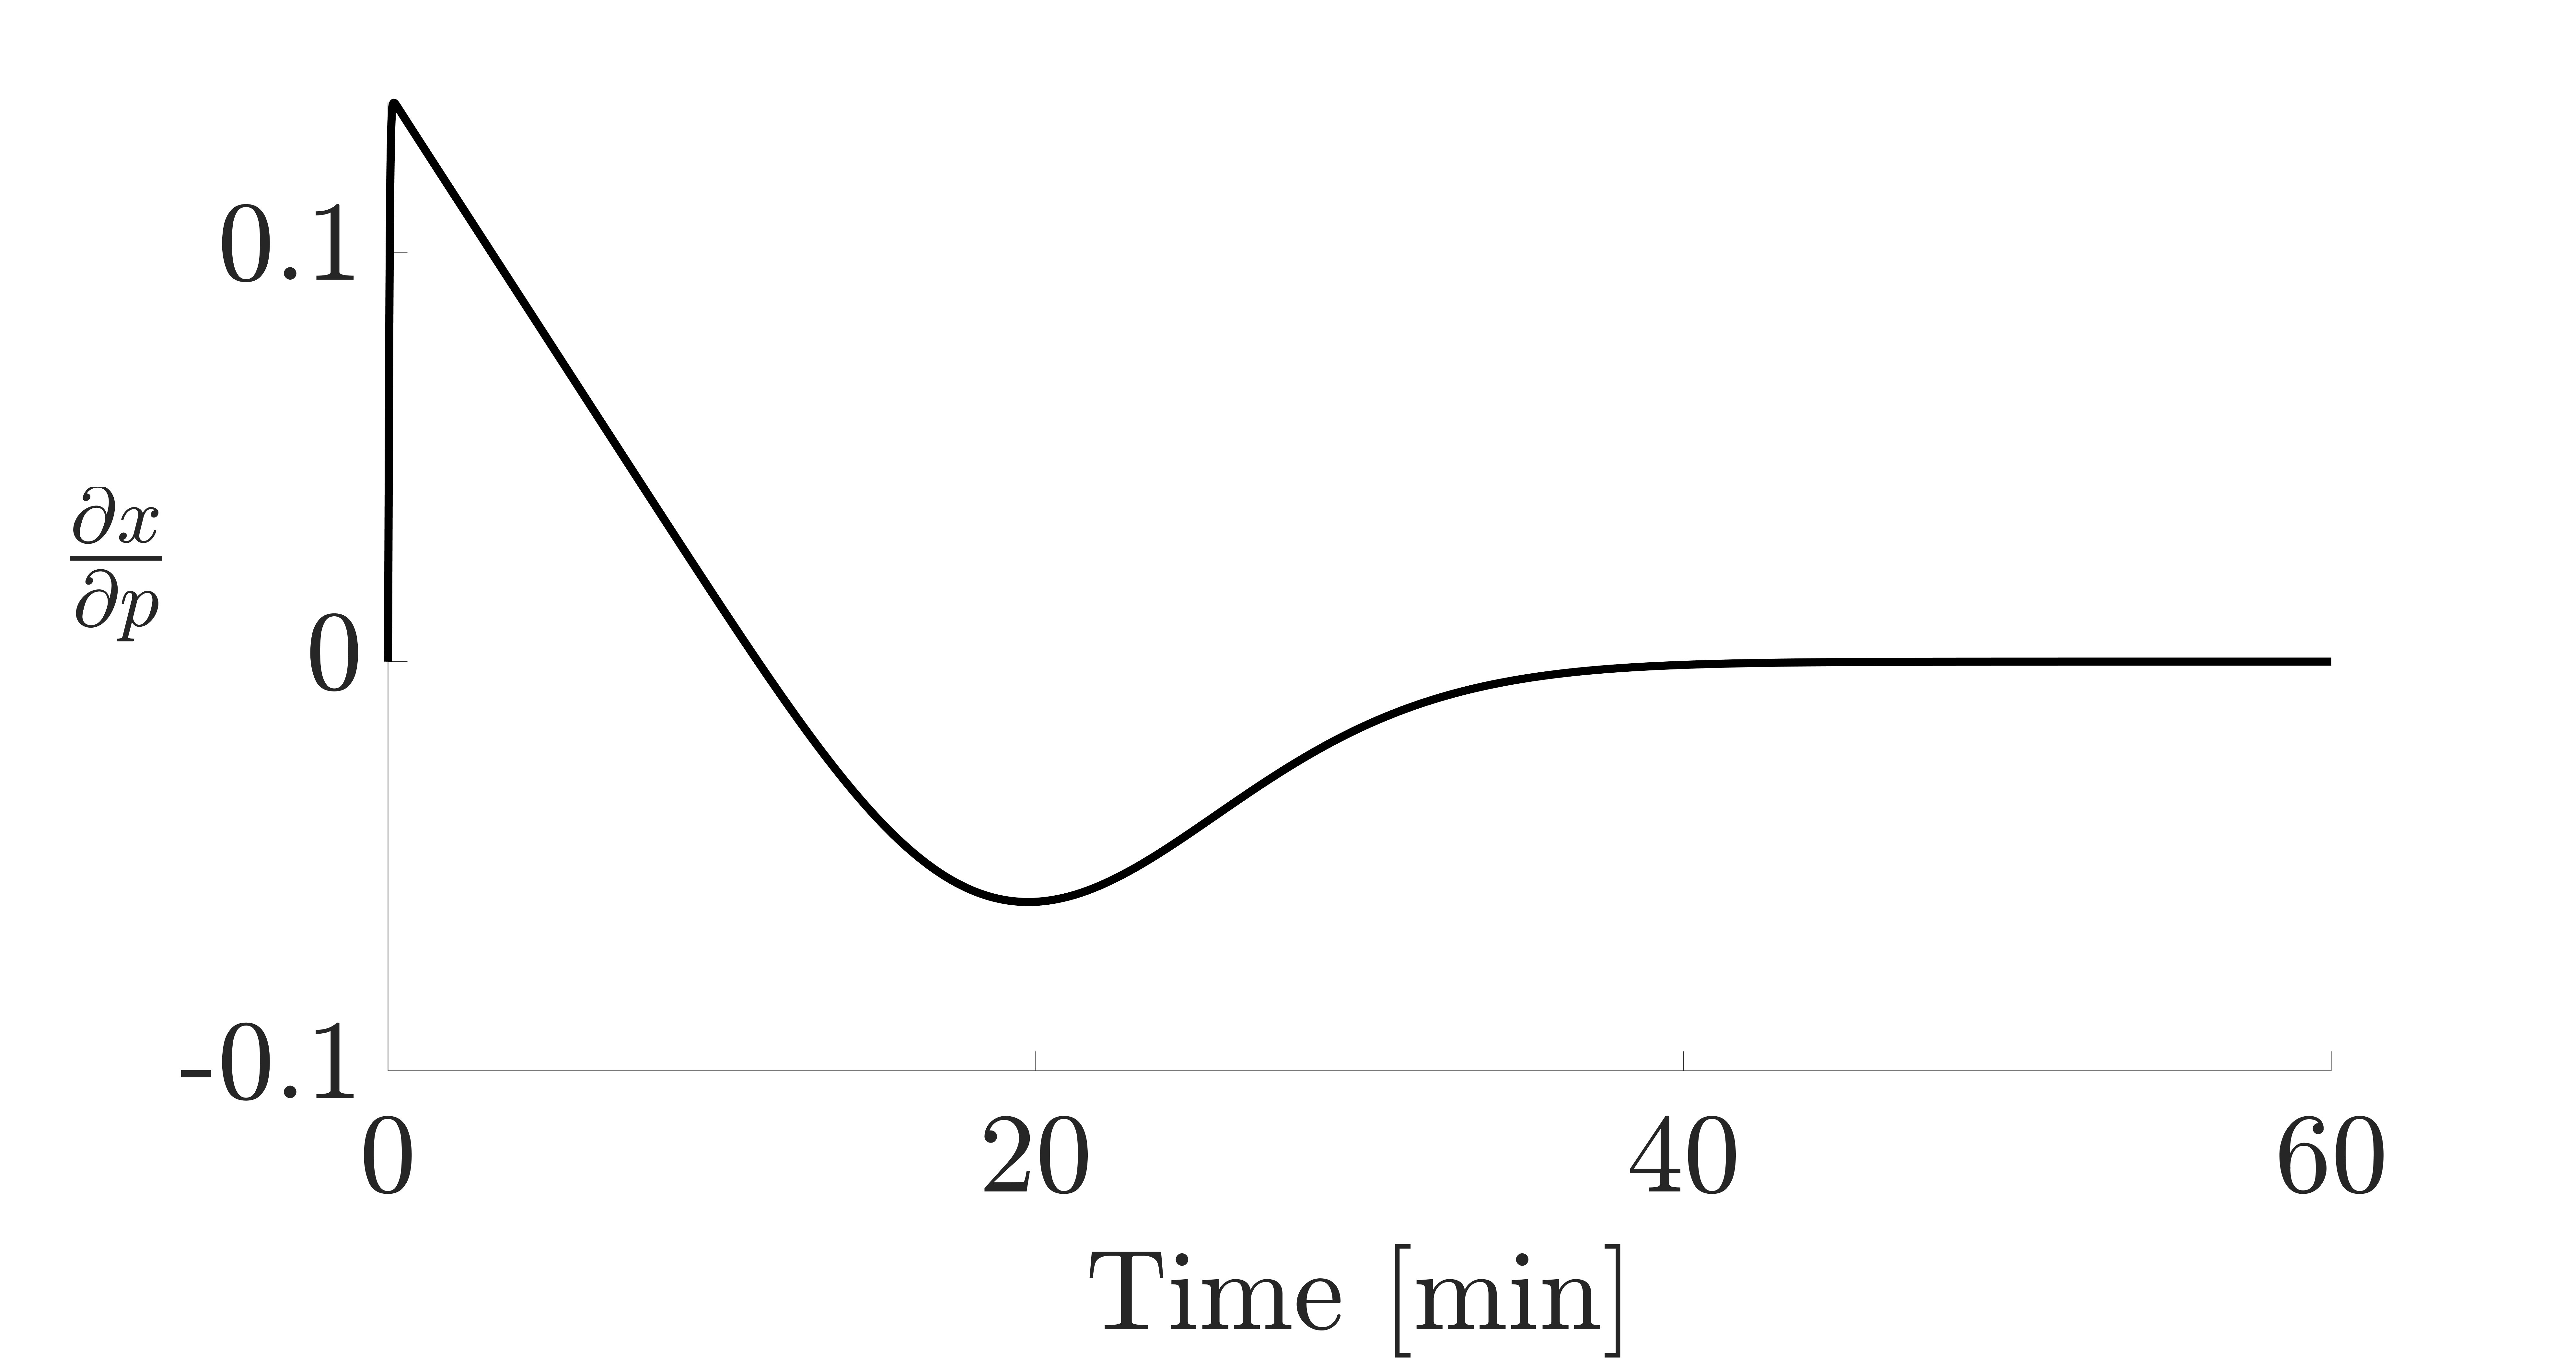
\includegraphics[width=0.32\linewidth]{Figures/Sensitivity/Plots/1_SS_R_P.png}
%			\end{tikzfigure}  
%			\captionof{figure}{Sensitivity with respect of the pressure}          
%			\begin{tikzfigure}
%				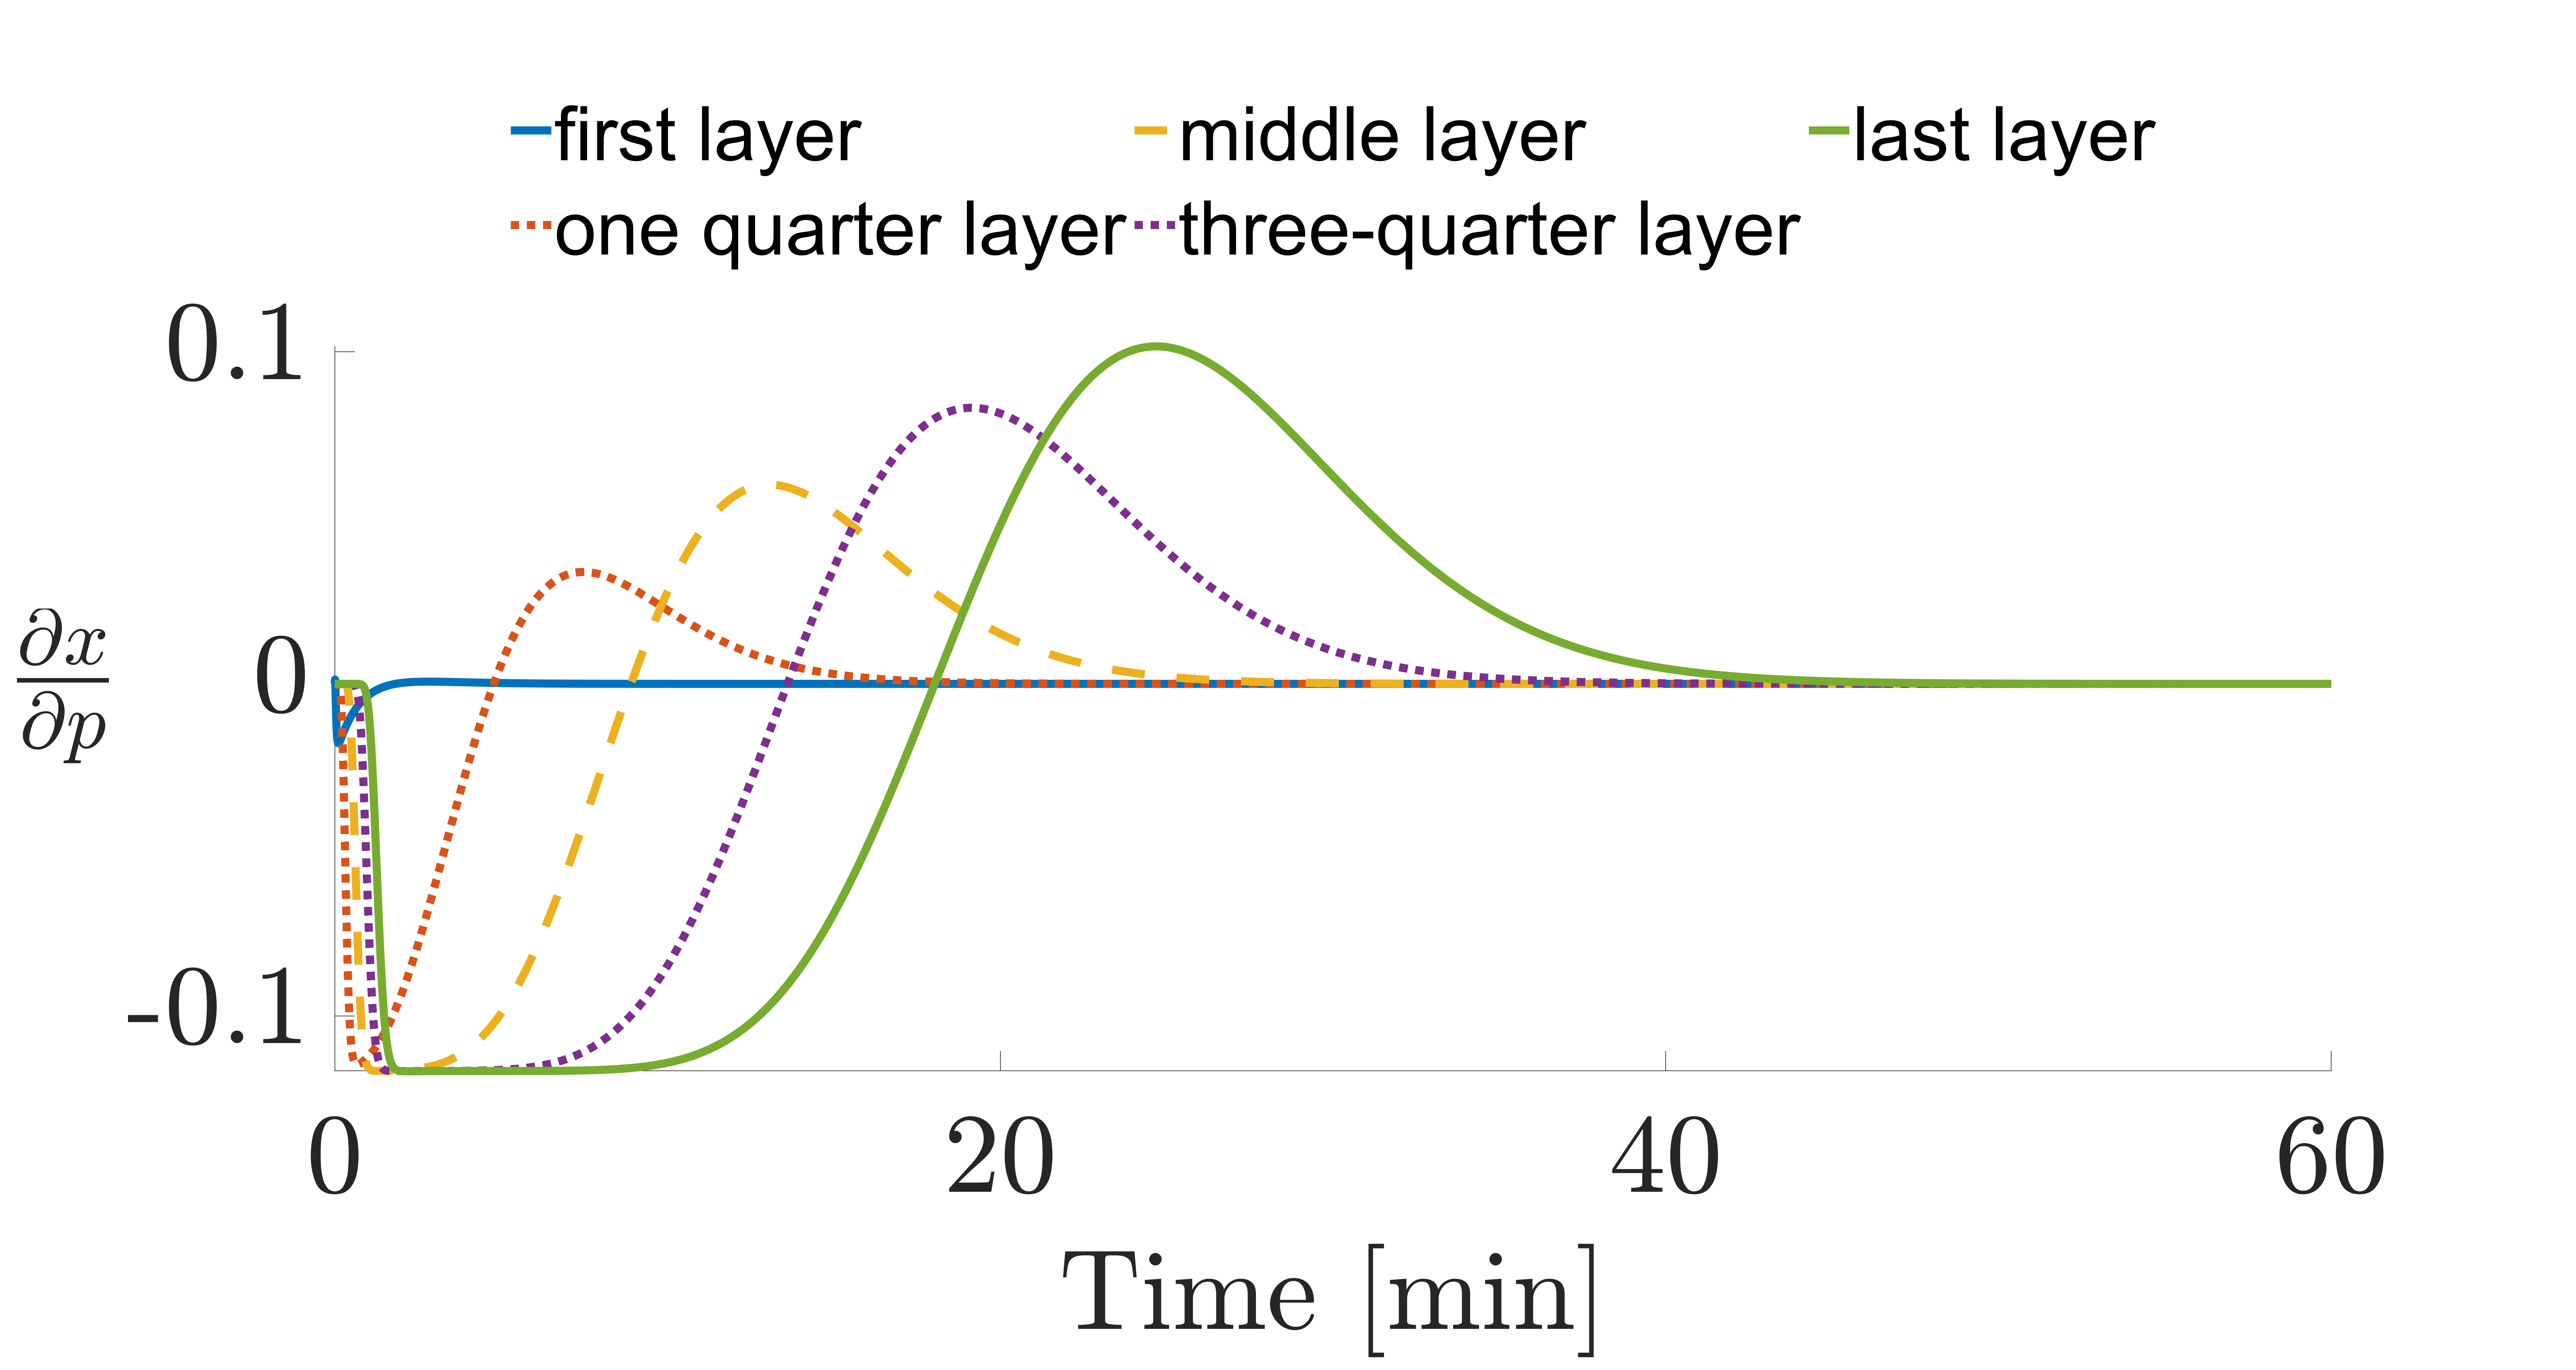
\includegraphics[width=0.32\linewidth]{Figures/Sensitivity/Imagesc/2_SS_R_T.png}
%				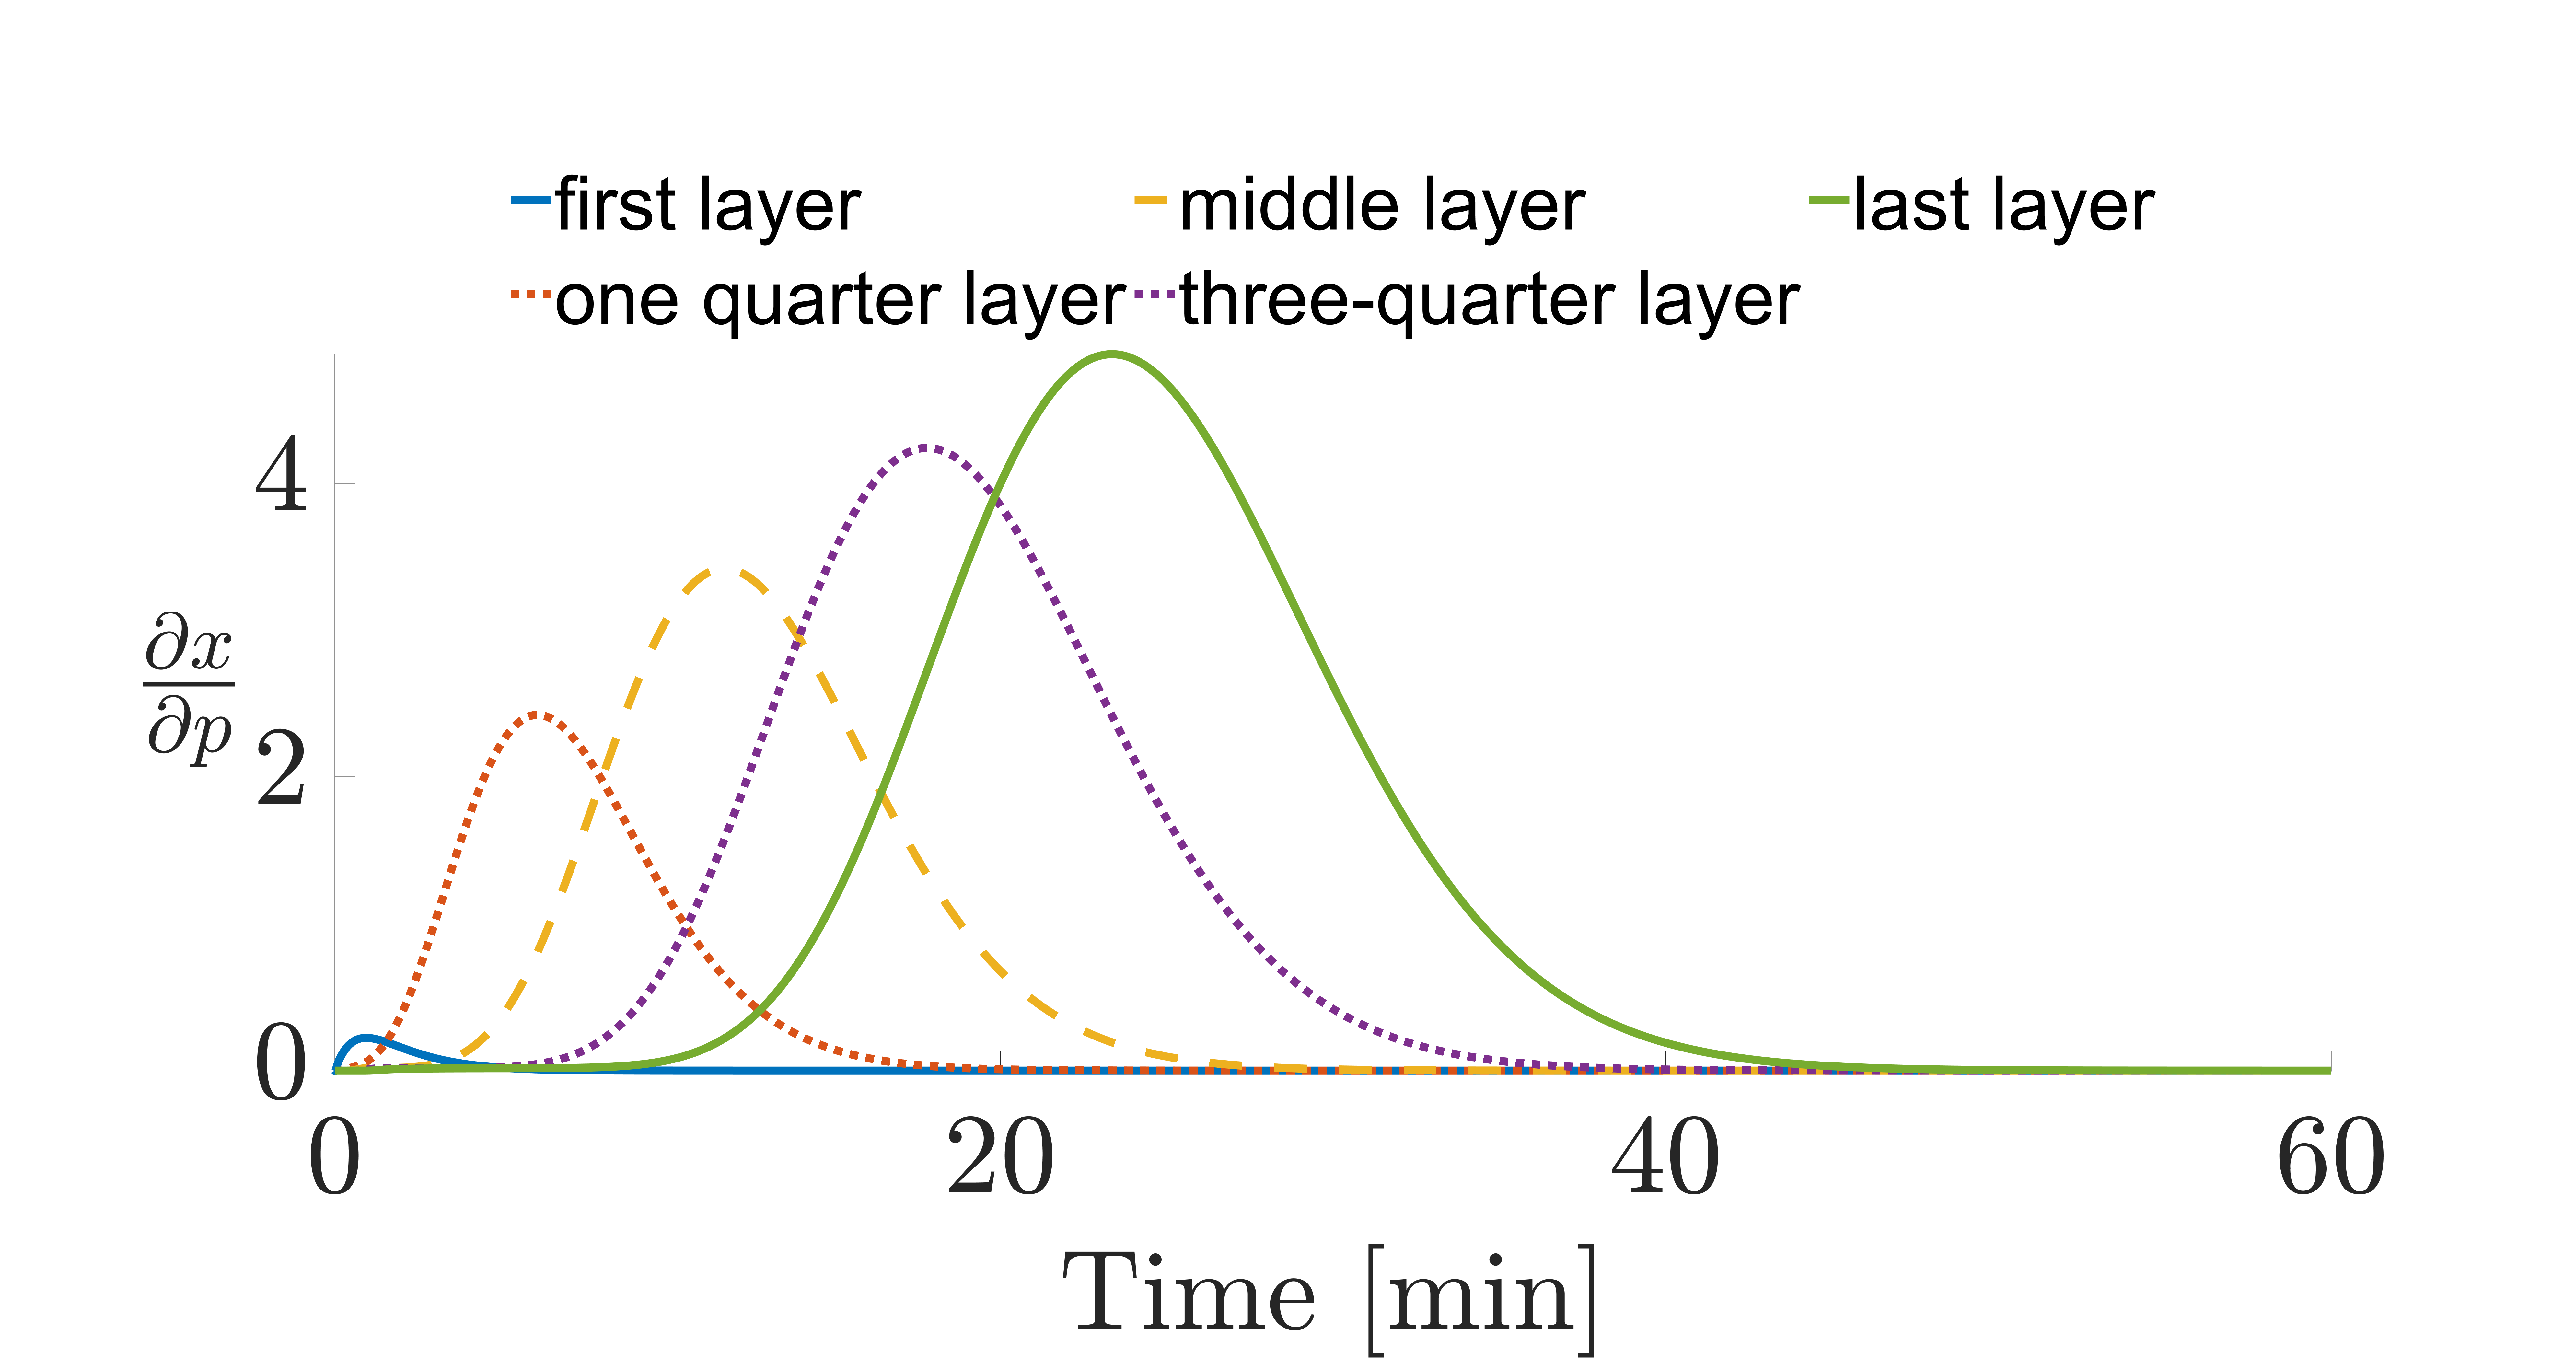
\includegraphics[width=0.32\linewidth]{Figures/Sensitivity/Imagesc/3_SS_R_T.png}
%				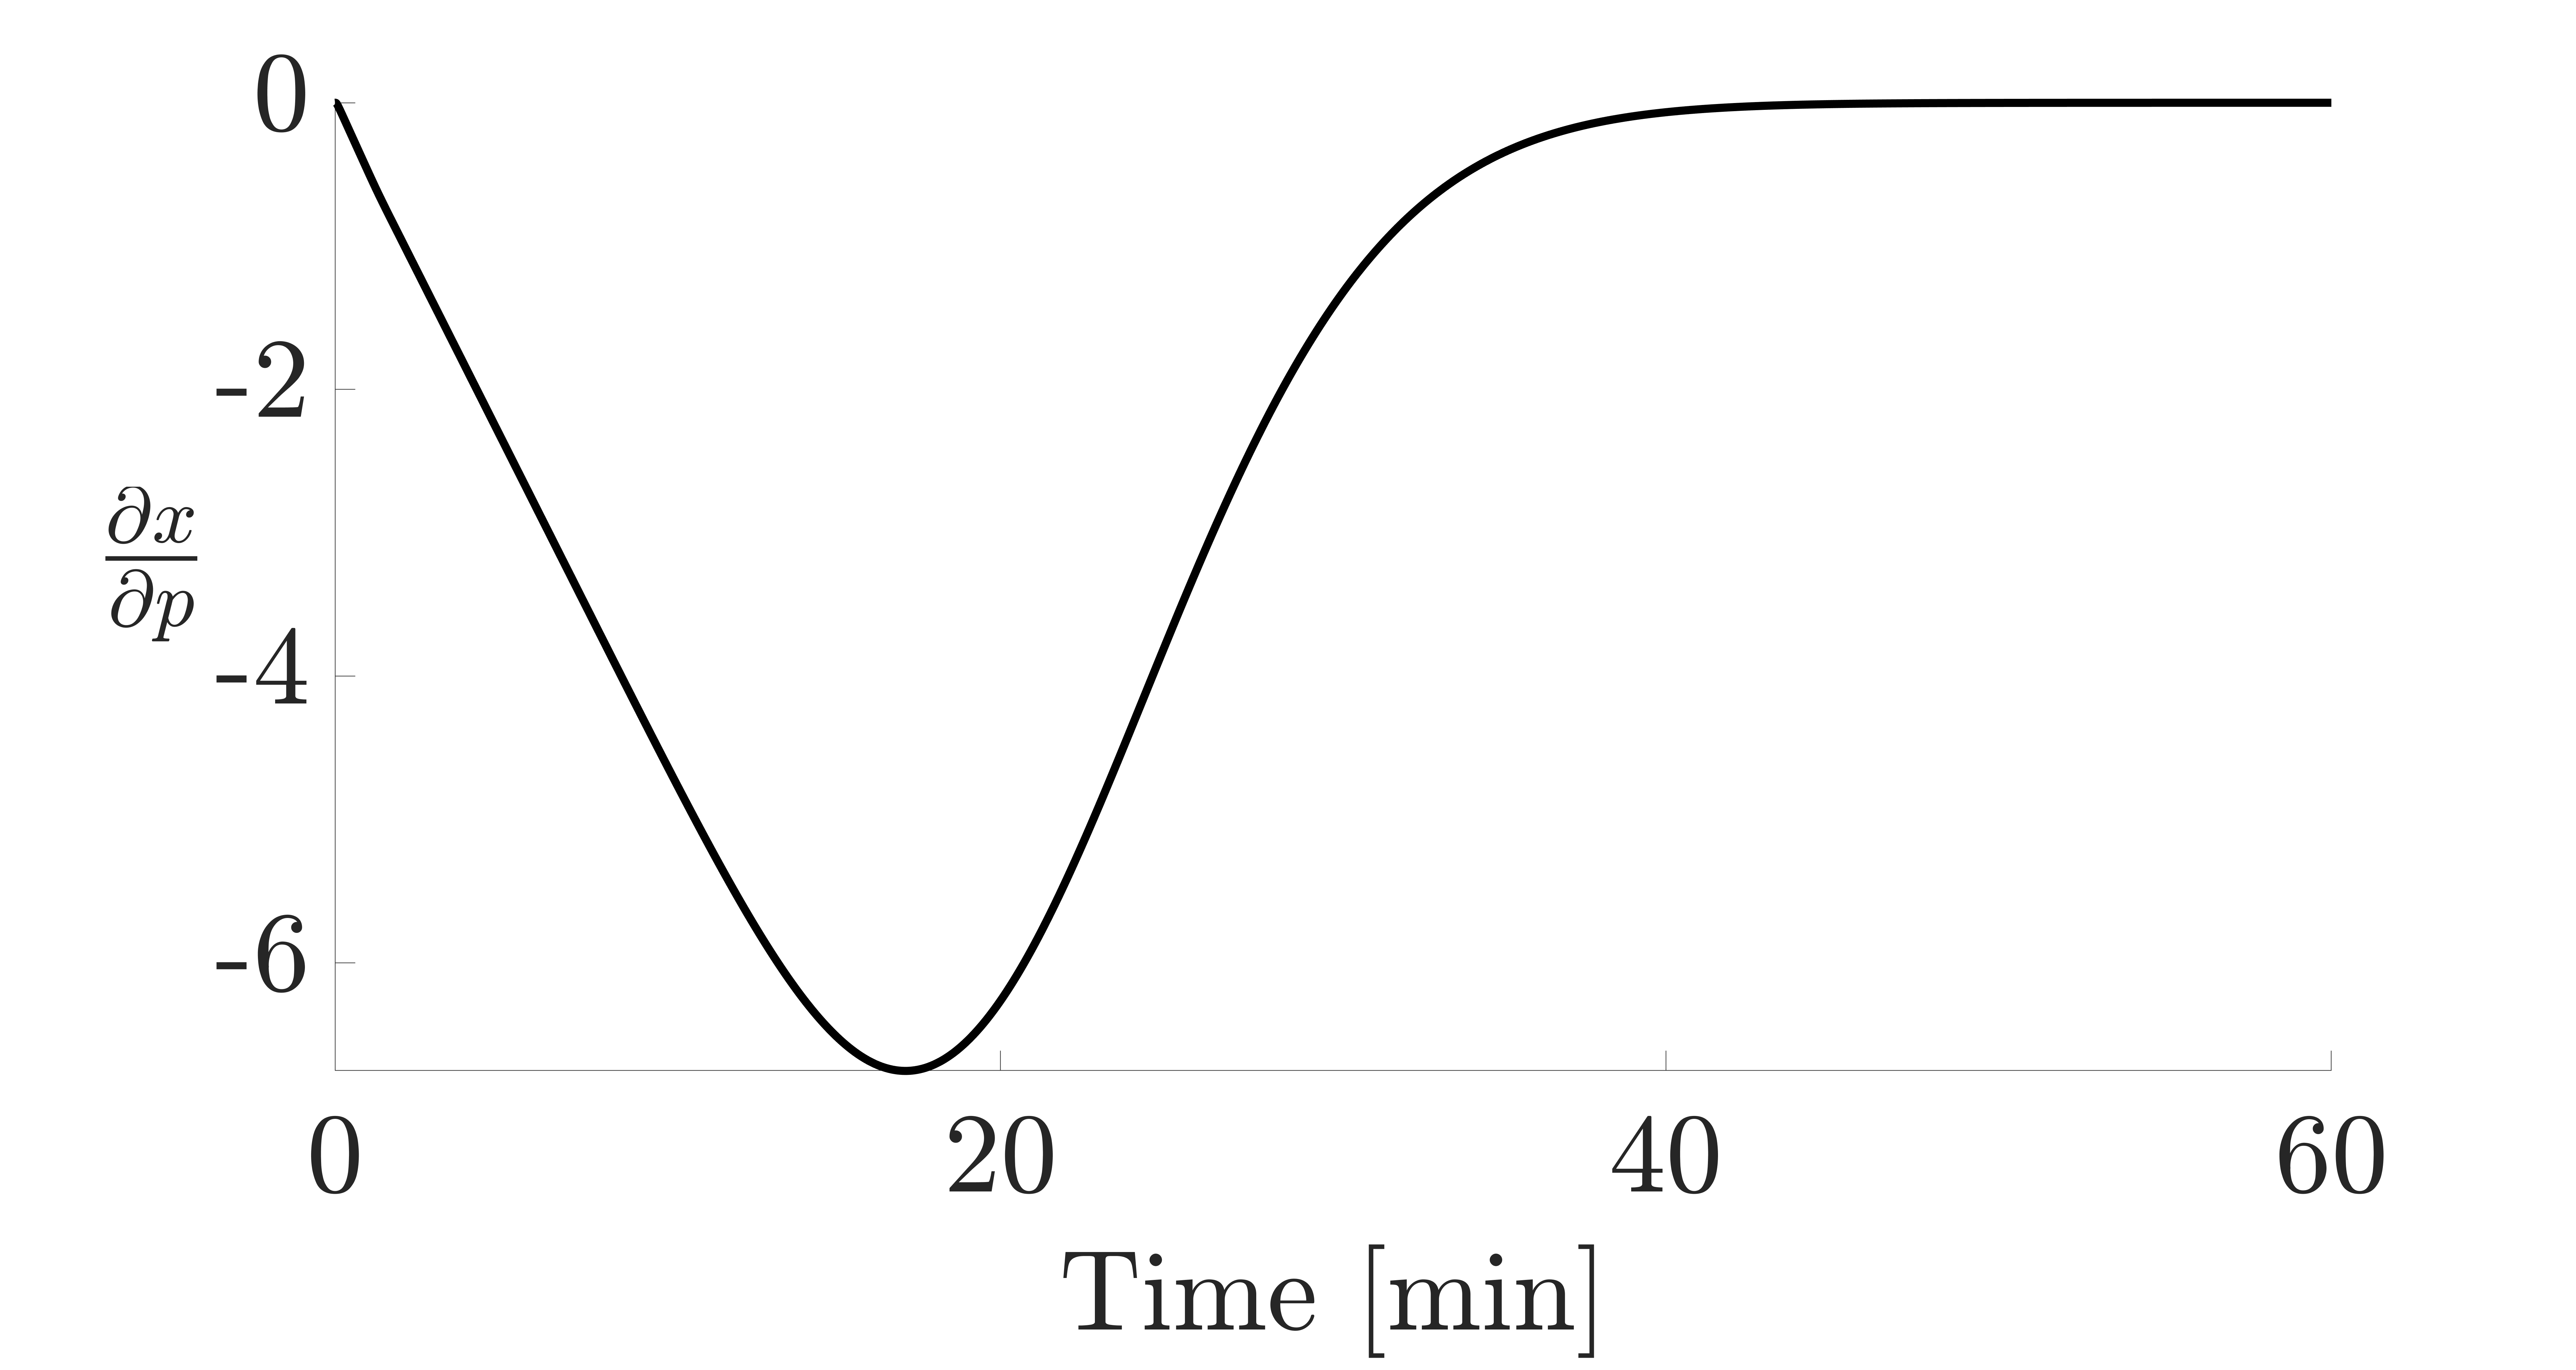
\includegraphics[width=0.32\linewidth]{Figures/Sensitivity/Plots/1_SS_R_T.png}
%			\end{tikzfigure}        	
%			\captionof{figure}{Sensitivity with respect to the inlet temperature}
%			\hrule
%			\begin{tikzfigure}
%				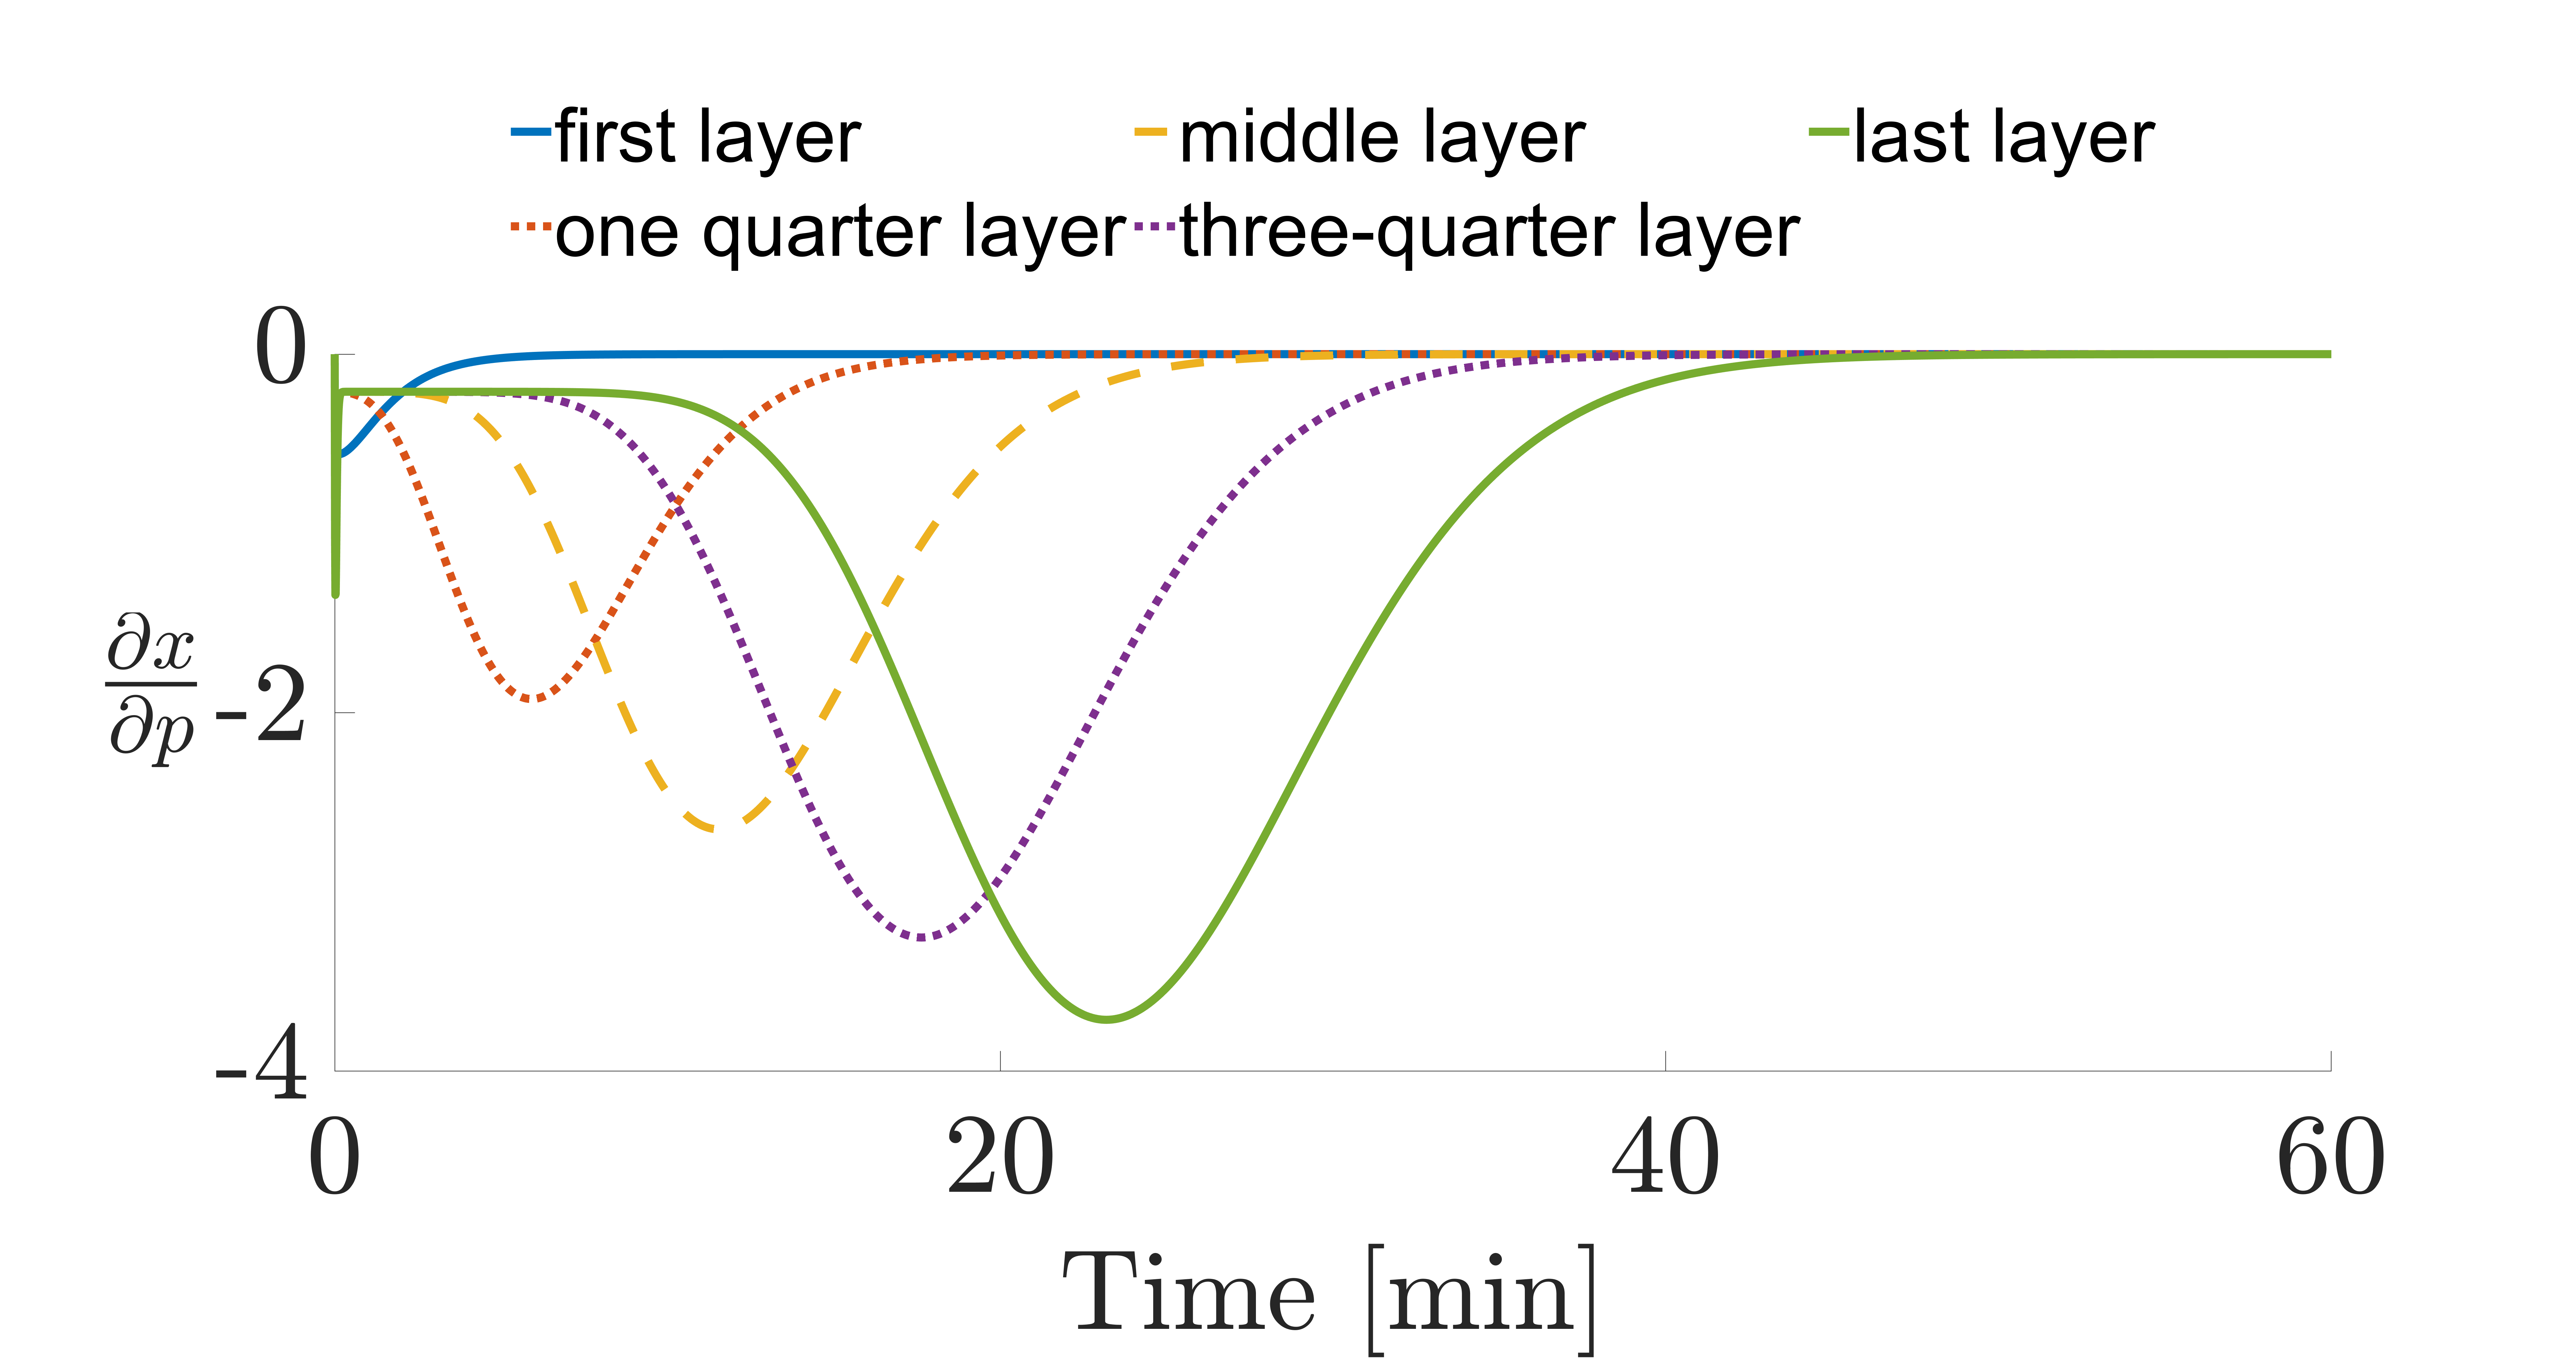
\includegraphics[width=0.32\linewidth]{Figures/Sensitivity/Imagesc/2_SS_R_epsi.png}
%				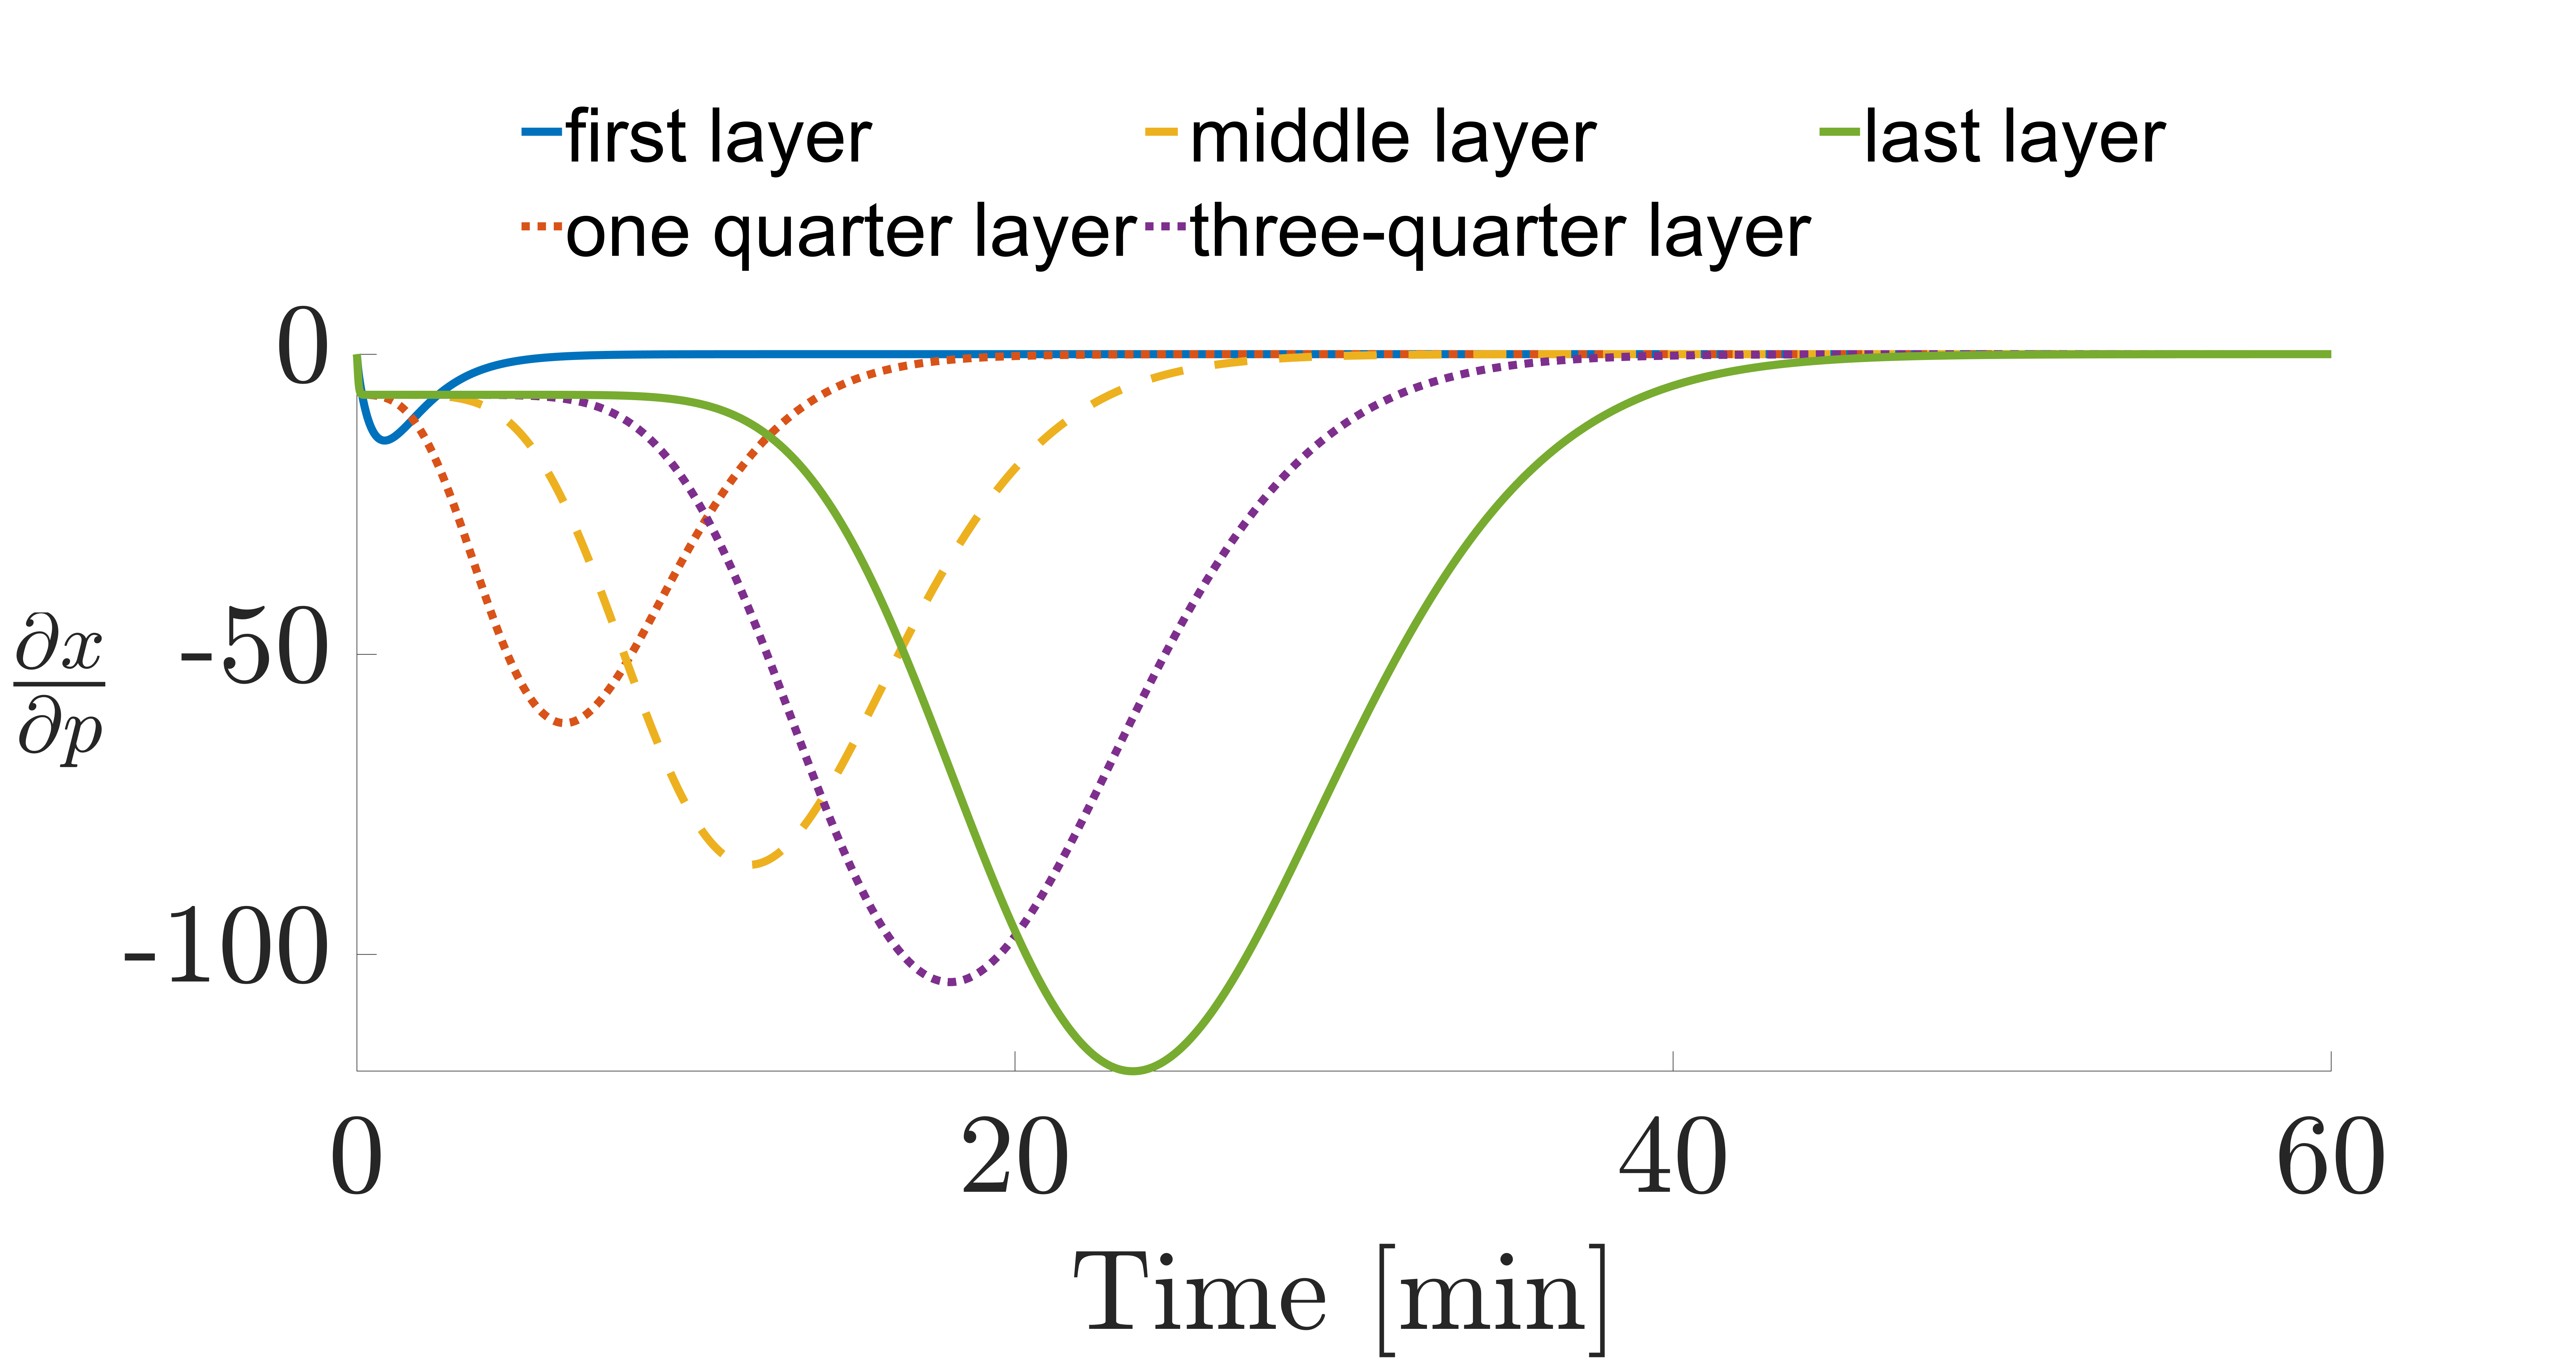
\includegraphics[width=0.32\linewidth]{Figures/Sensitivity/Imagesc/3_SS_R_epsi.png}
%				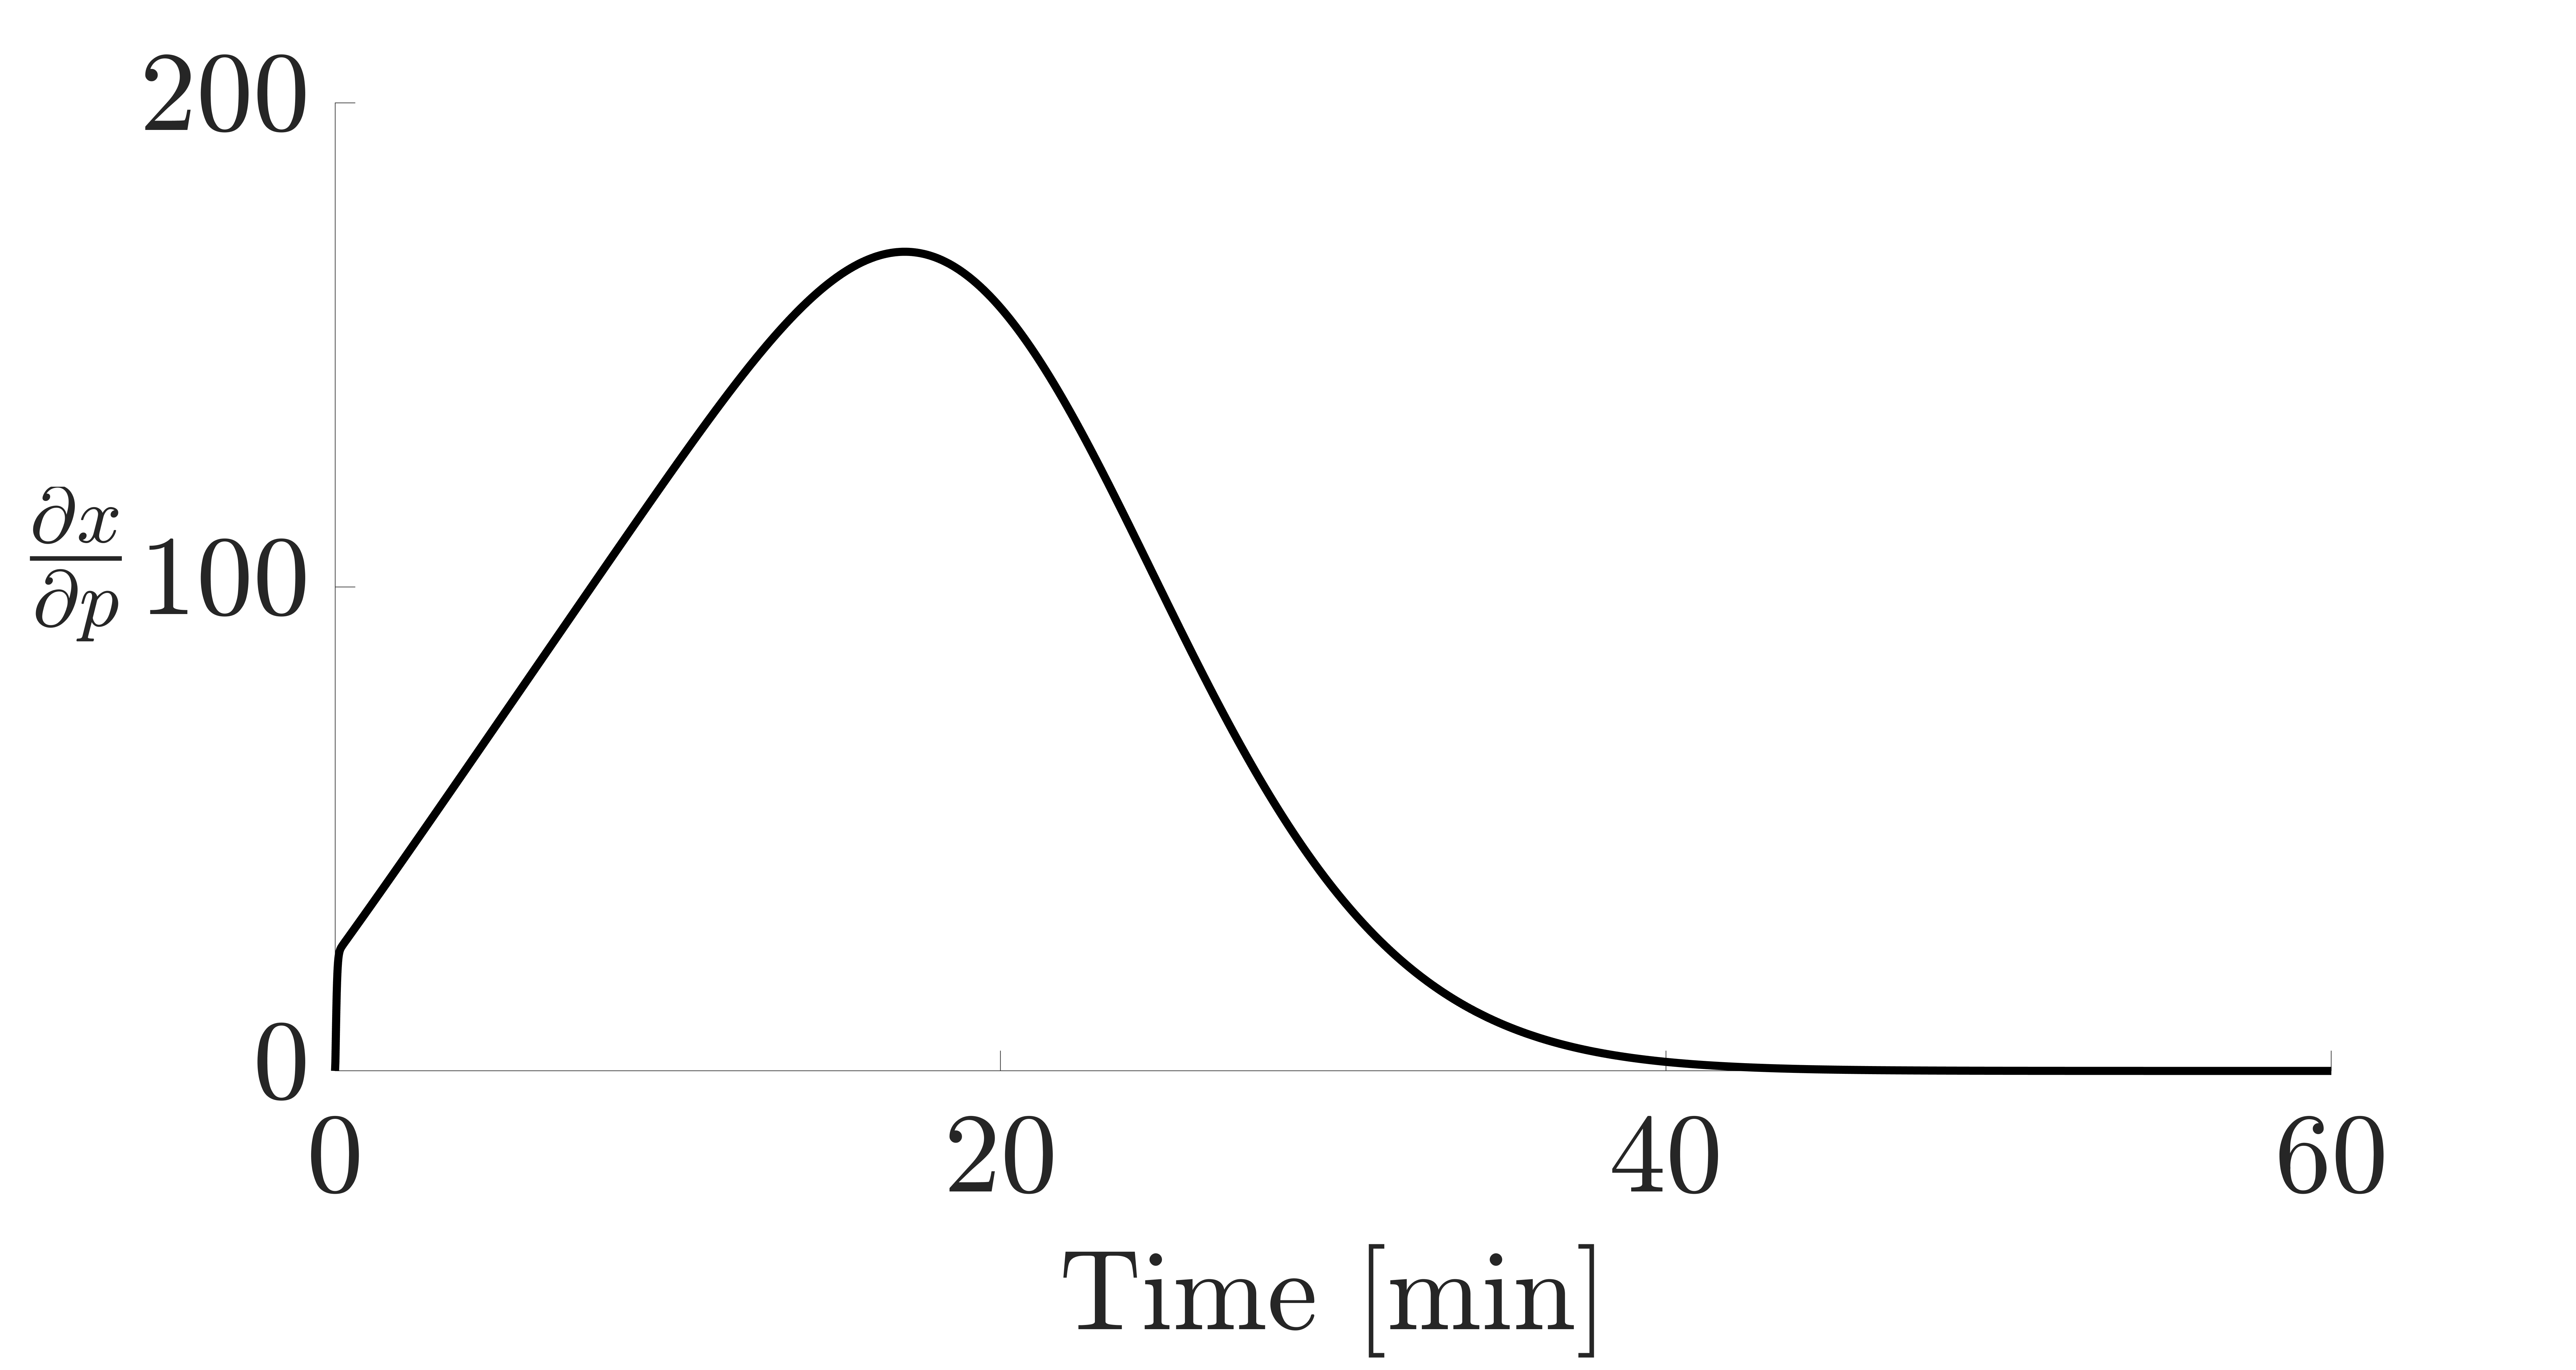
\includegraphics[width=0.32\linewidth]{Figures/Sensitivity/Plots/1_SS_R_epsi.png}
%				\caption{Yield sensitivity}
%			\end{tikzfigure}     
%			\captionof{figure}{Sensitivity with respect to the void fraction} 
		}
		
		\block{References}{
			\renewcommand{\bibsection}{}
			\bibliographystyle{unsrtnat}
			\bibliography{mybibfile}
			
		}
	\end{columns}
\end{document}
